\documentclass{mwrep}

% Polskie znaki
\usepackage{polski}
\usepackage[polish]{babel}
\usepackage[utf8]{inputenc}
\usepackage[T1]{fontenc}
\usepackage[utf8]{luainputenc}
\usepackage{lmodern}
\usepackage{indentfirst}

% Strona tytułowa
\usepackage{pgfplots}
\usepackage{siunitx}
\usepackage{paracol}
\usepackage{gensymb}

% Pływające obrazki
\usepackage{float}
\usepackage{svg}
\usepackage{pdfpages}
\usepackage{graphicx}
\usepackage{subcaption}

% table of contents refs
\usepackage{hyperref}
\usepackage{booktabs}
\usepackage{listings}
\usepackage{amsmath}
\usepackage{placeins}
\usepackage{xcolor}
\usepackage{cleveref}
\usepackage[toc, page]{appendix}


\usetikzlibrary{pgfplots.groupplots}
\sisetup{detect-weight,exponent-product=\cdot,output-decimal-marker={,},per-mode=symbol,binary-units=true,range-phrase={-},range-units=single}
\definecolor{szary}{rgb}{0.95,0.95,0.95}
%konfiguracje pakietu listings
\lstset{
	backgroundcolor=\color{szary},
	frame=single,
	breaklines=true,
}
\lstdefinestyle{customlatex}{
	basicstyle=\footnotesize\ttfamily,
	%basicstyle=\small\ttfamily,
}
\lstdefinestyle{customc}{
	breaklines=true,
	frame=tb,
	language=C,
	xleftmargin=0pt,
	showstringspaces=false,
	basicstyle=\small\ttfamily,
	keywordstyle=\bfseries\color{green!40!black},
	commentstyle=\itshape\color{purple!40!black},
	identifierstyle=\color{blue},
	stringstyle=\color{orange},
}
\lstdefinestyle{custommatlab}{
	%basicstyle=\fontsize{11}{13}\selectfont\ttfamily,
	captionpos=t,
	breaklines=true,
	frame=tb,
	xleftmargin=0pt,
	language=matlab,
	showstringspaces=false,
	%basicstyle=\footnotesize\ttfamily,
	basicstyle=\scriptsize\ttfamily,
	keywordstyle=\bfseries\color{green!40!black},
	commentstyle=\itshape\color{purple!40!black},
	identifierstyle=\color{blue},
	stringstyle=\color{orange},
}

%wymiar tekstu
\def\figurename{Rys.}
\def\tablename{Tab.}

%konfiguracja liczby p�ywaj�cych element�w
\setcounter{topnumber}{0}%2
\setcounter{bottomnumber}{3}%1
\setcounter{totalnumber}{5}%3
\renewcommand{\textfraction}{0.01}%0.2
\renewcommand{\topfraction}{0.95}%0.7
\renewcommand{\bottomfraction}{0.95}%0.3
\renewcommand{\floatpagefraction}{0.35}%0.5

\captionsetup{compatibility=false}

\SendSettingsToPgf
\title{\bf Sprawozdanie z projektu i ćwiczenia laboratoryjnego nr 4, zadanie nr 1 \vskip 0.1cm}
\author{Marcin Dolicher \\ Jakub Sikora \\ Robert Wojtaś}
\date{\today}
\pgfplotsset{compat=1.15}	
\begin{document}
\frenchspacing
\pagestyle{uheadings}

\makeatletter
\renewcommand{\maketitle}{\begin{titlepage}
		\begin{center}{
				\LARGE {\bf Politechnika Warszawska}}\\
            \vspace{0.4cm}
            \leftskip-0.9cm
            {\LARGE {\bf \mbox{Wydział Elektroniki i Technik Informacyjnych}}}\\
            \vspace{0.2cm}
            {\LARGE {\bf \mbox{Instytut Automatyki i Informatyki Stosowanej}}}\\
            
            \vspace{5cm}
            \leftskip-1.3cm
			{\bf \Huge \mbox{Projektowanie układów sterowania} \vskip 0.1cm}
		\end{center}
		\vspace{0.1cm}

		\begin{center}
			{\bf \LARGE \@title}
		\end{center}

		\vspace{9cm}
		\begin{paracol}{2}
			\addtocontents{toc}{\protect\setcounter{tocdepth}{1}}
			\subsection*{Zespół:}
			\bf{ \Large{ \noindent\@author \par}}
			\addtocontents{toc}{\protect\setcounter{tocdepth}{2}}

			\switchcolumn \addtocontents{toc}{\protect\setcounter{tocdepth}{1}}
			\subsection*{Prowadzący:}
			\bf{\Large{\noindent \mbox{mgr inż. Andrzej Wojtulewicz}}}
			\addtocontents{toc}{\protect\setcounter{tocdepth}{2}}

		\end{paracol}
		\vspace*{\stretch{6}}
		\begin{center}
			\bf{\large{Warszawa, \@date\vskip 0.1cm}}
		\end{center}
	\end{titlepage}
}
\makeatother
\maketitle
\tableofcontents

\part{Projekt}
%\chapter{Zbadanie poprawności podanego punktu pracy}
\label{pro1}

W pierwszej kolejności sprawdziliśmy poprawność podanego w projekcie 
punktu pracy. W stanie ustalonym spodziewamy się $u_{\mathrm{1}} = u_{\mathrm{2}} 
= u_{\mathrm{3}} = u_{\mathrm{4}} = y_{\mathrm{1}} = y_{\mathrm{2}} = 
y_{\mathrm{3}} = 0$. Za pomocą skryptu \verb+zad1.m+ dokonaliśmy sprawdzenia
czy podane wartości są poprawne. Skrypt ten wywołuje funkcję
\verb+symulacja_obiektu1+ z następującymi parametrami.

\lstset{language=Matlab,%
    breaklines=true,%
    morekeywords={matlab2tikz},
    keywordstyle=\color{blue},%
    morekeywords=[2]{1}, keywordstyle=[2]{\color{black}},
    identifierstyle=\color{black},%
    stringstyle=\color{mylilas},
    stringstyle=\color{magenta},
    commentstyle=\color{green},%
    showstringspaces=false,%without this there will be a symbol in the places where there is a space
    numbers=left,%
    numberstyle={\tiny \color{black}},% size of the numbers
    numbersep=9pt, % this defines how far the numbers are from the text
    emph=[1]{for,end,break},emphstyle=[1]\color{red}, %some words to emphasise
    %emph=[2]{word1,word2}, emphstyle=[2]{style},    
}

\begin{lstlisting}[style=custommatlab,frame=single,label={pro1},caption={Sprawdzenie poprawności podanego punktu pracy},captionpos=b]
    Upp1 = 0;
    Upp2 = 0;
    Upp3 = 0;
    Upp4 = 0;

    Ypp1 = 0;
    Ypp2 = 0;
    Ypp3 = 0;

    [y1, y2, y3] = symulacja_obiektu1(Upp1, Upp1, Upp1, Upp1, ...
                                      Upp2, Upp2, Upp2, Upp2, ...
                                      Upp3, Upp3, Upp3, Upp3, ...
                                      Upp4, Upp4, Upp4, Upp4, ...
                                      Ypp1, Ypp1, Ypp1, Ypp1, ...
                                      Ypp2, Ypp2, Ypp2, Ypp2, ...
                                      Ypp3, Ypp3, Ypp3, Ypp3);
\end{lstlisting}

W wyniku działania funkcji uzyskaliśmy wektor samych zer, które równe są wartościom wszystkich wyjść w punkcie pracy.
Jednoznacznie potwierdza to poprawność podanego punktu pracy.
%\chapter{Wyznaczenie odpowiedzi skokowych obiektu}
\label{zad2}

\section{Odpowiedź skokowa toru wejście-wyjście}
Eksperymenty wykonywane były z punktu pracy zdefiniowanego w zadaniu, przy sygnale zakłócenia $Z_{\mathrm{pp}} = 0$. Na wykresie \ref{zad2_odp_skok_input} możemy zaobserwować, że wraz z wzrostem wartości skoku rośnie również wartość odpowiedzi procesu $y[k]$. Zachowanie procesu jest zgodne 
z typową charakterystyką obiektów dynamicznych liniowych, w których wartość ustalona zmienia się liniowo wraz ze zmianą sygnału sterującego. 

\begin{figure}[t]
    \centering
    \begin{tikzpicture}
    \begin{axis}[
    width=0.98\textwidth,
    xmin=0.0,xmax=200,ymin=-1.5,ymax=1.5,
    xlabel={$k$},
    ylabel={$y[k]$},
    legend pos=south east,
    y tick label style={/pgf/number format/1000 sep=},
    ] 
    \addlegendentry{$\Delta u = \num{0,1}$},
    \addlegendentry{$\Delta u = \num{0,2}$}
    \addlegendentry{$\Delta u = \num{0,35}$},
    \addlegendentry{$\Delta u = \num{0,5}$},
    \addlegendentry{$\Delta u = \num{-0,1}$},
    \addlegendentry{$\Delta u = \num{-0,2}$},
    \addlegendentry{$\Delta u = \num{-0,35}$},
    \addlegendentry{$\Delta u = \num{-0,5}$},
    \addlegendimage{no markers,green}
	\addlegendimage{no markers,red}
	\addlegendimage{no markers,yellow}
	\addlegendimage{no markers,blue}
	\addlegendimage{no markers,black}
	\addlegendimage{no markers,orange}
	\addlegendimage{no markers,brown}
	\addlegendimage{no markers,violet}
    \addplot[green, semithick, thick] file{../data/zad2/zad2_input_output0.1.csv};
    \addplot[red, semithick, thick] file{../data/zad2/zad2_input_output0.2.csv};
    \addplot[yellow, semithick, thick] file{../data/zad2/zad2_input_output0.35.csv};
    \addplot[blue, semithick, thick] file{../data/zad2/zad2_input_output0.5.csv};
    \addplot[black, semithick, thick] file{../data/zad2/zad2_input_output-0.1.csv};
    \addplot[orange, semithick, thick] file{../data/zad2/zad2_input_output-0.2.csv};
    \addplot[brown, semithick, thick] file{../data/zad2/zad2_input_output-0.35.csv};
    \addplot[violet, semithick, thick] file{../data/zad2/zad2_input_output-0.5.csv};    
    \end{axis}
    \end{tikzpicture}
    \caption{Odpowiedzi procesu na skokową zmianę sygnału sterującego}
    \label{zad2_odp_skok_input}
\end{figure}

\section{Odpowiedź skokowa toru zakłócenie-wyjście}

Odpowiedź skokową toru zakłócenie-wyjście otrzymywaliśmy poprzez skokową zmianę zakłócenia. Eksperymenty wykonywane były ze stanu punktu pracy, w którym wszystkie sygnały wynosiły 0. Sygnał sterowania był stały podczas całej symulacji. Na wykresie \ref{zad2_odp_skok_disturbance} obserwujemy reakcję na zmiany zakłóceń i możemy stwierdzić, że jest ona podobna do tej otrzymanej przy zmianach sterowania, co tylko potwierdza nasze przypuszczenia o liniowości obiektu. 

\begin{figure}[b]
    \centering
    \begin{tikzpicture}
    \begin{axis}[
    width=0.98\textwidth,
    xmin=0.0,xmax=200,ymin=-1,ymax=1,
    xlabel={$k$},
    ylabel={$y[k]$},
    legend pos=south east,
    y tick label style={/pgf/number format/1000 sep=},
    ] 
    \addlegendentry{$\Delta z = \num{0,05}$},
    \addlegendentry{$\Delta z = \num{0,2}$}
    \addlegendentry{$\Delta z = \num{0,35}$},
    \addlegendentry{$\Delta z = \num{0,5}$},
    \addlegendentry{$\Delta z = \num{-0,05}$},
    \addlegendentry{$\Delta z = \num{-0,2}$},
    \addlegendentry{$\Delta z = \num{-0,35}$},
    \addlegendentry{$\Delta z = \num{-0,5}$},
    \addlegendimage{no markers,green}
	\addlegendimage{no markers,red}
	\addlegendimage{no markers,yellow}
	\addlegendimage{no markers,blue}
	\addlegendimage{no markers,black}
	\addlegendimage{no markers,orange}
	\addlegendimage{no markers,brown}
	\addlegendimage{no markers,violet}
    \addplot[green, semithick, thick] file{../data/zad2/zad2_disturbance_output0.05.csv};
    \addplot[red, semithick, thick] file{../data/zad2/zad2_disturbance_output0.2.csv};
    \addplot[yellow, semithick, thick] file{../data/zad2/zad2_disturbance_output0.35.csv};
    \addplot[blue, semithick, thick] file{../data/zad2/zad2_disturbance_output0.5.csv};
    \addplot[black, semithick, thick] file{../data/zad2/zad2_disturbance_output-0.05.csv};
    \addplot[orange, semithick, thick] file{../data/zad2/zad2_disturbance_output-0.2.csv};
    \addplot[brown, semithick, thick] file{../data/zad2/zad2_disturbance_output-0.35.csv};
    \addplot[violet, semithick, thick] file{../data/zad2/zad2_disturbance_output-0.5.csv};    
    \end{axis}
    \end{tikzpicture}
    \caption{Odpowiedzi procesu na skokową zmianę sygnału zaklócenia}
    \label{zad2_odp_skok_disturbance}
\end{figure}

\section{Wyznaczenie charakterystyki statycznej $y(u,z)$}
Wyznaczenie charakterystyki $y(u,z)$ rozpoczęliśmy od wyznaczenia charakterystyk $y(u)$ i $y(z)$. 
Na dalszym etapie zadania pomogło to w określeniu wzmocnień statycznych torów wejście-wyjście, zakłócenie-wyjśćie. 

Aby otrzymać wykres charakterystyki statycznej obiektu w zależności od 
dwóch argumentów należało przeprowadzić symulacje dla każdej 
wartości sygnałów $u$ oraz $d$ i zapamiętaniu wartości 
nasycenia sygnału $y$. Program, który realizujący zadanie to 
\verb+zad2_static_surface.m+ wykonywał wspomniane działania, 
a wyniki zapisywał do tablicy z wartościami charakterystyki statycznej. 
Wynik można zobaczyć na rysunku \ref{zad2_static_surf}.\\
\indent{} Wykres przedstawia płaszczyznę $y(u,z)$. Skoro powstały wykres 
jest płaszczyzną to można wywnioskować, że mamy do czynienia z obiektem liniowym. 


\chapter{Dobieranie nastawów regulatorów PID}
\label{zad5}

\section{Strojenie regulatora PID}
\label{zad5_PID_wykresy}
W celu dobrania optymalnych parametrów regulatora, wyszliśmy od parametrów uzyskanych metodą
Zieglera-Nicholsa a następnie ręcznie dostroiliśmy poszczególne parametry tak aby uzyskać
jak najlepszy efekty końcowy. Eksperyment ten polegał na znalezieniu takiego wzmocnienia $K_{r}$, 
zwanego wzmocnieniem krytycznym, dla którego obiekt wpadał w niegasnące oscylacje o okresie $T_{k}$. 

Cały proces dobierania parametrów składał się z następujących kroków:
\begin{center}
\begin{enumerate}
    \item Wyznaczenie wzmocnienia $K_{\mathrm{k}}$ i okresu oscylacji $T_{\mathrm{k}}$
    \item Wyliczenie parametrów regulatora
    \item Ręczna poprawa wartości wzmocnienia członu proporcjonalnego $K_{\mathrm{r}}$
    \item Ręczna poprawa wartości parametru członu całkującego $T_{\mathrm{i}}$
    \item Ręczna poprawa wartości parametru członu różniczkującego $T_{\mathrm{d}}$
\end{enumerate}
\end{center}

Chcąc znaleźć jeszcze lepsze nastawy regulatora, po wyznaczeniu parametrów za pomocą metody Zieglera-Nicholsa, zastosowaliśmy metodę eksperymentalną. W której jakość regulacji ocenialiśmy jakościowo (na podstawie przebiegów sygnałów na wykresach) oraz ilościowo, za pomocą wskaźnika jakości regulacji danego wzorem:
\begin{equation}
E=\sum_{k=0}^{K_{konc}}(y^{zad}[k]-y[k])^{2}
\end{equation}


\subsection{Wyznaczenie wzmocnienia $K_{\mathrm{k}}$ i okresu oscylacji $T_{\mathrm{k}}$}
\label{zad5_wyznaczanie_parametrow_zn}
Na początku doprowadziliśmy układ do granicy stabilności, czyli momentu
w którym zaczęły pojawiać się niegasnące oscylacje. Zrealizowaliśmy to
zwiększając współczynnik wzmocnienia $K_{\mathrm{r}}$ przy wyłączonych członach 
całkującym i różniczkującym. Iteracyjnie wyznaczaliśmy nowe wartości wzmocnienia,
zwiększając jego wartość w przypadku gasnących oscylacji oraz zmniejszając w przypadku
niestabilnej odpowiedzi obiektu.

Gdy ostatecznie zaobserwowaliśmy niegasnące oscylacje zapisaliśmy aktualne wzmocnienie 
jako wzmocnienie krytyczne $K_{k}$ i zmierzyliśmy okres oscylacji drgań 
krytycznych $T_{k}$ ($K_{k} = 1,8 \hspace{0.3 cm} T_{k}=18,5 $). Wiedząc że okres próbkowania procesu 
wynosi $\num{0,5}s$, a zmierzony okres oscylacji wynosił $\num{37}$ próbek, wyliczyliśmy że
okres drgań krytycznych równa się $T_{k}=18,5s$. 

\begin{figure}[t]
    \centering
    \begin{tikzpicture}
    \begin{axis}[
    width=0.98\textwidth,
    xmin=0,xmax=500,ymin=3.7, ymax=4.3,
    xlabel={$k$},
    ylabel={$y[k]$},
    %xtick={0, 100, 200, 300, 400, 500},
    %ytick={3.9, 4, 4.1, 4.2, 4.3, 4.4},
    legend pos=south east,
    y tick label style={/pgf/number format/1000 sep=},
    ]
    \addplot[blue, semithick] file{../data/Zad5_figure_data/zad5_PID_setpoint_exampleK_1.8_Ti_1000000000000_Td_0.csv};
    \addplot[red, semithick] file{../data/Zad5_figure_data/zad5_PID_output_exampleK_1.8_Ti_1000000000000_Td_0.csv};
    \addlegendentry{$y^{zad}[k]$},
    \addlegendentry{$y[k]$},
    \addlegendimage{no markers, blue}
	\addlegendimage{no markers, red}
    \end{axis}
    \end{tikzpicture}
    \caption{Niegasnące oscylacje wyjścia obiektu przy wzmocnieniu krytycznym}
    \label{zad5_niegasnace_oscylacje}
\end{figure}

\begin{figure}[b]
    \centering
    \begin{tikzpicture}
    \begin{axis}[
    width=0.98\textwidth,
    xmin=0,xmax=500,ymin=0.25, ymax=0.75,
    xlabel={$k$},
    ylabel={$u[k]$},
    %xtick={0, 0.4, 0.5, 0.6, 0.7},
    %ytick={3.5, 3.75, 4, 4.25, 4.5},
    legend pos=south east,
    y tick label style={/pgf/number format/1000 sep=},
    ]
    \addplot[const plot, blue, semithick] file{../data/Zad5_figure_data/zad5_PID_input_exampleK_1.8_Ti_1000000000000_Td_0.csv};
    \legend{$u[k]$}
    \end{axis}
    \end{tikzpicture}
    \caption{Przebieg sygnału sterującego }
    \label{zad5_niegasnace_oscylacje_ster}
\end{figure}
\FloatBarrier

\subsection{Wyliczenie wstępnych parametrów regulatora}
\label{zad5_regulator_zn}
Dobierając nastawy według metody Zieglera-Nicholsa, 
stosowaliśmy wzory do obliczenia parametrów regulatora PID: 

\begin{equation}
\label{zad5_zn_wzory}
K_{\mathrm{r}}=\num{0,6}K_{\mathrm{k}} \hspace{1cm} T_{\mathrm{i}}=\num{0,5} \hspace{1cm} T_{\mathrm{k}} T_{\mathrm{d}}=\num{0,12} T_{\mathrm{k}}
\end{equation}
gdzie:
\begin{center}
\begin{itemize}
    \item $K_{\mathrm{k}}$ - wzmocnienie krytyczne
    \item $T_{\mathrm{k}}$ - okres oscylacji
\end{itemize}
\end{center}

Wyliczone wartości liczbowe parametrów:
\begin{center}
$K_{r}=\num{1,08} \hspace{0.5 cm}
T_{i}=\num{9,25}   \hspace{0.5 cm}
T_{d}=\num{2,22}$
\end{center}

Regulator z parametrami wyznaczonymi przy pomocy metody opisanej przez panów Johna Zieglera
i Nathaniela Nicholsa, nadal charakteryzuje się niegasnącymi oscylacjami. Takie 
przebiegi sygnałów są nieakceptowalne, dlatego w dalszych krokach ręcznie modyfikowaliśmy 
wartości parametrów. 

Na rysunku \ref{zad5_zn_regulator} przedstawiono przebiegu wartości zadanej oraz
wyjścia obiektu z widocznie przedstawionymi oscylacjami wokół wartości zadanej.
Rysunek \ref{zad5_zn_sterowanie} przedstawia zmianę sygnału sterującego
generowanego przez regulator.

Tak nastrojony regulator PID bardzo słabo radzi sobie z utrzymywaniem sygnału wyjściowego
procesu na poziomie wartości zadanej. Niegasnące oscylacje nie pozwalają na zastosowanie
tego zestawu parametrów do regulacji procesem. Dla zadanej trajektorii testowej, obliczony 
wskaźnik jakości regulacji wyniósł $E = \num{5,8385}$. Pomimo swoich wad, regulator ten jest 
dobrym punktem wyjścia dla metody eksperymentalnej.

\begin{figure}[t]
    \centering
    \begin{tikzpicture}
    \begin{axis}[
    width=0.98\textwidth,
    xmin=0,xmax=600,ymin=3.7, ymax=4.4,
    xlabel={$k$},
    ylabel={$y[k]$},
    %xtick={0.3, 0.4, 0.5, 0.6, 0.7},
    %ytick={3.5, 3.75, 4, 4.25, 4.5},
    legend pos=south east,
    y tick label style={/pgf/number format/1000 sep=},
    ]
    \addplot[blue, semithick] file{../data/zad5_multiplejumps/zad5_PID_setpoint_exampleK_1.08_Ti_9.25_Td_2.22_E_5.8385.csv};
    \addplot[red, semithick] file{../data/zad5_multiplejumps/zad5_PID_output_exampleK_1.08_Ti_9.25_Td_2.22_E_5.8385.csv};
    \addlegendentry{$y^{zad}[k]$},
    \addlegendentry{$y[k]$},
    \addlegendimage{no markers, blue}
	\addlegendimage{no markers, red}
    \end{axis}
    \end{tikzpicture}
    \caption{Przebieg procesu sterowanego za pomocą regulatora z parametrami wyznaczonymi za pomocą metody Zieglera-Nicholsa}
    \label{zad5_zn_regulator}
\end{figure}

\begin{figure}[b]
    \centering
    \begin{tikzpicture}
    \begin{axis}[
    width=0.98\textwidth,
    xmin=0.0,ymin=0.3, xmax= 600,
    xlabel={$k$},
    ylabel={$u[k]$},
    %xtick={0.3, 0.4, 0.5, 0.6, 0.7},
    %ytick={3.5, 3.75, 4, 4.25, 4.5},
    legend pos=south east,
    y tick label style={/pgf/number format/1000 sep=},
    ]
    \addplot[const plot, blue, semithick] file{../data/zad5_multiplejumps/zad5_PID_input_exampleK_1.08_Ti_9.25_Td_2.22_E_5.8385.csv};
    \legend{$u[k]$}
    \end{axis}
    \end{tikzpicture}
    \caption{Przebieg sygnału sterującego regulatora z parametrami wyznaczonymi za pomocą metody Zieglera-Nicholsa}
    \label{zad5_zn_sterowanie}
\end{figure}
\FloatBarrier

\subsection{Ręczna poprawa wartości wzmocnienia członu proporcjonalnego $K_{\mathrm{r}}$ }
\label{zad5_poprawa_Kr}
\subsubsection{Wzmocnienie regulatora $\mathbf{K_{\mathrm{r}}}=\num{0,75}$}
W pierwszej kolejności skupiliśmy się na zmianie parametru $K_{\mathrm{r}}$.
Zmniejszenie $K_{\mathrm{r}}$ do wartości $\num{0.75}$ sprawiło że pozbyliśmy się oscylacji. Czas regulacji
wyniósł około 100 próbek. Dodatkowo, sygnał wyjściowy procesu nie cechuje się przeregulowaniem,
czyli przekroczenie wartości zadanej. Wyjście obiektu już nie oscyluje tak jak to było w przypadku regulatora z \ref{zad5_regulator_zn},
jak i została przywrócona stabilność procesu. Sygnał sterujący cechuje się oscylacjami przy zmianach
wartości zadanej, co powoduje nierówny przebieg wyjścia procesu.
Wartość wskaźnika jakości regulacji dla tego regulatora przy tej samej
testowej trajektorii zadanej wyniosła $E=\num{5,6914}$, co jest niewielką poprawą w stosunku 
do bazowego regulatora.
Przebiegi sygnału wyjściowego jaki i sygnału sterującego, odbiegały od pożądanych.

Wykres \ref{zad5_1_K_odp} przedstawia przebiegi wyjścia procesu oraz trajektorii zadanej.
Na rysunku \ref{zad5_1_zmiana_K} przedstawiliśmy przebieg sygnału sterującego generowanego przez regulator.

\subsubsection{Wzmocnienie regulatora $\mathbf{K_{\mathrm{r}}}=\num{0,6}$}
Zmniejszenie $K_{\mathrm{r}}$ do poziomu $\num{0,6}$ spowodowało wizualną poprawę odpowiedzi układu 
na zmianę wartości zadanej. Przebieg sygnału wyjściowego wygładził się, proces w łagodniejszy sposób
dociera do wartości zadanej. Czas regulacji niie zmienił się w porównaniu do poprzedniego regulatora.
Przebieg sygnału sterującego również uległ wygładzeniu, chociaż oscylacje nie zniknęły w całości.
Wartość wskaźnika jakości regulacji dla tego 
przypadku wyniosła $E=\num{6.1449}$, co zaskakująco, jest wartością większą w porównaniu do poprzedniego 
$K_{\mathrm{r}}$ regulatora. Łagodniejszy przebieg wyjścia powoduje zwiększenie sumy kwadratów uchybu.

Wykres \ref{zad5_2_K_odp} przedstawia przebiegi wyjścia procesu oraz trajektorii zadanej.
Na rysunku \ref{zad5_2_zmiana_K} przedstawiliśmy przebieg sygnału sterującego generowanego przez regulator.

\subsubsection{Wzmocnienie regulatora $\mathbf{K_{\mathrm{r}}}=\num{0,5}$}
Na wykresach \ref{zad5_3_K_odp} i \ref{zad5_3_zmiana_K} przedstawiono przebiegi powstałe 
dla regulatora z wzmocnieniem $ K_{\mathrm{r}} = \num{0,5}$. Sygnał sterujący praktycznie nie
oscyluje, natomiast sygnał wyjściowy ma jeszcze łagodniejszy przebieg co niestety sprawia że czas regulacji 
nieznacznie wzrósł. Niestety, wskaźnik jakości 
regulacji wzrósł do wartości $E=\num{6,5814}$. Zauważyliśmy, że jego wartość rośnie przy zmniejszaniu  
parametru $ K_{\mathrm{r}}$, dlatego postanowiliśmy 
ostatecznie przyjąć wartość $K_{\mathrm{r}} = \num{0,5}$ i przejść do manipulowania 
pozostałymi parametrami. Dalsze zmniejszanie nie spowoduje 
znaczącej poprawy przebiegów a jedynie pogorszy wskaźnik jakości regulacji. 

%%%%%%%%%%%%%%%%%%%%%%%%%%%%% wykresy dla k = 0.75

\begin{figure}[t]
    \centering
    \begin{tikzpicture}
    \begin{axis}[
    width=0.98\textwidth,
    xmin=0,xmax=600,ymin=3.8, ymax=4.4,
    xlabel={$k$},
    ylabel={$y[k]$},
    %xtick={0.3, 0.4, 0.5, 0.6, 0.7},
    %ytick={3.5, 3.75, 4, 4.25, 4.5},
    legend pos=south east,
    y tick label style={/pgf/number format/1000 sep=},
    ]
    \addplot[blue, semithick] file{../data/zad5_multiplejumps/P/zad5_PID_setpoint_exampleK_0.75_Ti_9.25_Td_2.22_E_5.6914.csv};
    \addplot[red, semithick] file{../data/zad5_multiplejumps/P/zad5_PID_output_exampleK_0.75_Ti_9.25_Td_2.22_E_5.6914.csv};
    \addlegendentry{$y^{zad}[k]$},
    \addlegendentry{$y[k]$},
    \addlegendimage{no markers, blue}
	\addlegendimage{no markers, red}
    \end{axis}
    \end{tikzpicture}
    \caption{Przebieg procesu sterowanego za pomocą regulatora z 
    parametrami \mbox{$K_{\mathrm{r}} = \num{0,75}$; $T_{\mathrm{i}} = \num{9,25}$; $T_{\mathrm{d}} = \num{2,22}$}}
    \label{zad5_1_K_odp}
\end{figure}

\begin{figure}[b]
    \centering
    \begin{tikzpicture}
    \begin{axis}[
    width=0.98\textwidth,
    xmin=0.0, ymin=0.44, xmax=600, ymax=0.68,
    xlabel={$k$},
    ylabel={$u[k]$},
    %xtick={0.3, 0.4, 0.5, 0.6, 0.7},
    %ytick={3.5, 3.75, 4, 4.25, 4.5},
    legend pos=south east,
    y tick label style={/pgf/number format/1000 sep=},
    ]
    \addplot[const plot, blue, semithick] file{../data/zad5_multiplejumps/P/zad5_PID_input_exampleK_0.75_Ti_9.25_Td_2.22_E_5.6914.csv};
    \legend{$u[k]$}
    \end{axis}
    \end{tikzpicture}
    \caption{Przebieg sygnału sterującego generowanego przez regulator z 
    parametrami \mbox{$K_{\mathrm{r}} = \num{0,75}$; $T_{\mathrm{i}} = \num{9,25}$; $T_{\mathrm{d}} = \num{2,22}$}}
    \label{zad5_1_zmiana_K}
\end{figure}
\FloatBarrier

%%%%%%%%%%%%%%%%%%%%%%%%%%%%% wykresy dla k = 0.6


\begin{figure}[t]
    \centering
    \begin{tikzpicture}
    \begin{axis}[
    width=0.98\textwidth,
    xmin=0,xmax=600,ymin=3.8, ymax=4.4,
    xlabel={$k$},
    ylabel={$y[k]$},
    %xtick={0.3, 0.4, 0.5, 0.6, 0.7},
    %ytick={3.5, 3.75, 4, 4.25, 4.5},
    legend pos=south east,
    y tick label style={/pgf/number format/1000 sep=},
    ]
    \addplot[blue, semithick] file{../data/zad5_multiplejumps/P/zad5_PID_setpoint_exampleK_0.6_Ti_9.25_Td_2.22_E_6.1449.csv};
    \addplot[red, semithick] file{../data/zad5_multiplejumps/P/zad5_PID_output_exampleK_0.6_Ti_9.25_Td_2.22_E_6.1449.csv};
    \addlegendentry{$y^{zad}[k]$},
    \addlegendentry{$y[k]$},
    \addlegendimage{no markers, blue}
	\addlegendimage{no markers, red}
    \end{axis}
    \end{tikzpicture}
    \caption{Przebieg procesu sterowanego za pomocą regulatora z 
    parametrami \mbox{$K_{\mathrm{r}} = \num{0,6}$; $T_{\mathrm{i}} = \num{9,25}$; $T_{\mathrm{d}} = \num{2,22}$}}
    \label{zad5_2_K_odp}
\end{figure}

\begin{figure}[b]
    \centering
    \begin{tikzpicture}
    \begin{axis}[
    width=0.98\textwidth,
    xmin=0.0,ymin=0.44, xmax=600, ymax=0.68,
    xlabel={$k$},
    ylabel={$u[k]$},
    %xtick={0.3, 0.4, 0.5, 0.6, 0.7},
    %ytick={3.5, 3.75, 4, 4.25, 4.5},
    legend pos=south east,
    y tick label style={/pgf/number format/1000 sep=},
    ]
    \addplot[const plot, blue, semithick] file{../data/zad5_multiplejumps/P/zad5_PID_input_exampleK_0.6_Ti_9.25_Td_2.22_E_6.1449.csv};
    \legend{$u[k]$}
    \end{axis}
    \end{tikzpicture}
    \caption{Przebieg sygnału sterującego generowanego przez regulator z 
    parametrami \mbox{$K_{\mathrm{r}} = \num{0,6}$; $T_{\mathrm{i}} = \num{9,25}$; $T_{\mathrm{d}} = \num{2,22}$}}
    \label{zad5_2_zmiana_K}
\end{figure}
\FloatBarrier

%%%%%%%%%%%%%%%%%%%%%% wykresy dla k = 0.5

\begin{figure}[t]
    \centering
    \begin{tikzpicture}
    \begin{axis}[
    width=0.98\textwidth,
    xmin=0,xmax=600, ymin=3.8, ymax=4.4,
    xlabel={$k$},
    ylabel={$y[k]$},
    %xtick={0.3, 0.4, 0.5, 0.6, 0.7},
    %ytick={3.5, 3.75, 4, 4.25, 4.5},
    legend pos=south east,
    y tick label style={/pgf/number format/1000 sep=},
    ]
    \addplot[blue, semithick] file{../data/zad5_multiplejumps/P/zad5_PID_setpoint_exampleK_0.5_Ti_9.25_Td_2.22_E_6.5814.csv};
    \addplot[red, semithick] file{../data/zad5_multiplejumps/P/zad5_PID_output_exampleK_0.5_Ti_9.25_Td_2.22_E_6.5814.csv};
    \addlegendentry{$y^{zad}[k]$},
    \addlegendentry{$y[k]$},
    \addlegendimage{no markers, blue}
	\addlegendimage{no markers, red}
    \end{axis}
    \end{tikzpicture}
    \caption{Przebieg procesu sterowanego za pomocą regulatora z 
    parametrami \mbox{$K_{\mathrm{r}} = \num{0,5}$; $T_{\mathrm{i}} = \num{9,25}$; $T_{\mathrm{d}} = \num{2,22}$}}
    \label{zad5_3_K_odp}
\end{figure}

\begin{figure}[b]
    \centering
    \begin{tikzpicture}
    \begin{axis}[
    width=0.98\textwidth,
    xmin=0.0,ymin=0.44, xmax=600, ymax=0.68,
    xlabel={$k$},
    ylabel={$u[k]$},
    %xtick={0.3, 0.4, 0.5, 0.6, 0.7},
    %ytick={3.5, 3.75, 4, 4.25, 4.5},
    legend pos=south east,
    y tick label style={/pgf/number format/1000 sep=},
    ]
    \addplot[const plot, blue, semithick] file{../data/zad5_multiplejumps/P/zad5_PID_input_exampleK_0.5_Ti_9.25_Td_2.22_E_6.5814.csv};
    \legend{$u[k]$}
    \end{axis}
    \end{tikzpicture}
    \caption{Przebieg sygnału sterującego generowanego przez regulator z 
    parametrami \mbox{$K_{\mathrm{r}} = \num{0,5}$; $T_{\mathrm{i}} = \num{9,25}$; $T_{\mathrm{d}} = \num{2,22}$}}
    \label{zad5_3_zmiana_K}
\end{figure}
\FloatBarrier

\subsection{Ręczna poprawa wartości czasu zdwojenia $T_{\mathrm{i}}$ }
\label{zad5_poprawa_Ti}

\subsubsection{Czas zdwojenia regulatora $\mathbf{T_{\mathrm{i}}}=\num{8,25}$}
W pierwszej kolejności postanowiliśmy minimalnie zmniejszyć wartość czasu zdwojenia
aby sprawdzić jak niewielkie zmiany tego parametru wpływają na końcowe przebiegi.
Okazuje się że zmniejszenie parametru $\mathbf{T_{\mathrm{i}}}=\num{8,25}$, bardzo
pozytywnie wpływa na przebiegi sygnałów wejściowego i wyjściowego. Nie występuje przeregulowanie
a czas regulacji został skrócony. Wartość wskaźnika jakości równa jest $E = \num{6,1901}$, co jest poprawą
w stosunku do poprzednio omawianego regulatora.

Przebiegi sygnału wyjściowego z zaznaczoną trajektorią zadaną oraz sygnału wejściowego znajdują się 
odpowiednio na rysunkach \ref{zad5_1_Ti_odp} i \ref{zad5_1_zmiana_Ti}.

\subsubsection{Czas zdwojenia regulatora $\mathbf{T_{\mathrm{i}}}=\num{7,25}$}
Idąc drogą obraną przy pierwszym regulatorze, postanowiliśmy jeszcze bardziej zmniejszyć 
czas zdwojenia $T_{\mathrm{i}}$. W kolejnej iteracji obraliśmy wartość parametru
$T_{\mathrm{i}}=\num{7,25}$. Zastosowanie takiej wartości spowodowało że przebieg 
sygnału wyjściowego jeszcze szybciej zbiegł do wartości zadanej. Większy wpływ członu całkującego
sprawia że regulator agresywniej podąża za trajektorią zadaną co objawia się pojawieniem 
niewielkiego przeregulowania i zwiększoną zrywnością sygnału sterującego. Nasze jakościowe 
rozważania potwierdza wskaźnik jakości regulacji którego wartość dla tego eksperymentu
wyniósł $E=\num{5,8298}$ co jest znacząco lepszym wynikiem niż przy $T_{\mathrm{i}}=\num{8,25}$.

Przebieg wyjścia procesu w porównaniu do wartości zadanej znajduje się na rysunku \ref{zad5_2_Ti_odp}.
Wyjście omawianego regulatora znajduje się na wykresie przedstawionym na rysunku \ref{zad5_2_zmiana_Ti}. 

\subsubsection{Czas zdwojenia regulatora $\mathbf{T_{\mathrm{i}}}=\num{6,25}$}
Kontynuując rozważania na temat czasu zdwojenia, zdecydowaliśmy się na jeszcze większe zmniejszenie 
parametru $T_{\mathrm{i}}$. Tym razem wybraliśmy wartość $T_{\mathrm{i}}=\num{6,25}$. Przebieg 
wyjścia procesu charakteryzuje się delikatnym przeregulowaniem, jednak dzięki temu udało się
jeszcze bardziej zredukować czas regulacji. Sygnał sterujący jest charakteryzuje się
większą agresywnością, co objawia się poprzez duże piki przy zmianie wartości zadanej.
Mimo wizualnie gorzej wyglądającego przebiegu wyjścia, wskaźnik jakości regulacji osiągnął najmniejszą
wartość $E=\num{5,5257}$. Przebieg wyjścia obiektu znajduje się na wykresie \ref{zad5_3_Ti_odp}. 
Przebieg sygnału sterującego znajduje się na rysunku \ref{zad5_3_zmiana_Ti}.

\subsubsection{Czas zdwojenia regulatora $\mathbf{T_{\mathrm{i}}}=\num{5,25}$}
Kolejną próbę wykonaliśmy dla regulatora z czasem zdwojenia $T_{\mathrm{i}}=\num{5,25}$. Pomimo
jeszcze lepszej wartości wskaźnika regulacji $E=\num{5,3567}$, to przebiegi sygnału wyjściowego i wejściowego
powodują że musimy odrzucić ten regulator. Bardzo duża zrywność regulatora powoduje że 
sygnał sterujący nasyca się na górnych ograniczeniach przy większych skokach wartości zadanej. Co więcej,
wyjście obiektu cechuje się zwiększonym przeregulowaniem i porównywalnym czasem regulacji. Omawiane przebiegi
znajdują się na rysunkach \ref{zad5_4_Ti_odp} i \ref{zad5_4_zmiana_Ti}. 

Biorąc pod uwagę powyższe rozważania, zdecydowaliśmy się na pozostanie przy wartości parametru $T_{\mathrm{i}} = \num{7,25}$.
Minimalnie przeregulowanie postaramy się zniwelować za pomocą parametru $T_{\mathrm{d}}$. 

%%%%%%%%%%% Ti = 8.25

\begin{figure}[t]
    \centering
    \begin{tikzpicture}
    \begin{axis}[
    width=0.98\textwidth,
    xmin=0,xmax=600, ymin=3.8, ymax=4.4,
    xlabel={$k$},
    ylabel={$y[k]$},
    %xtick={0.3, 0.4, 0.5, 0.6, 0.7},
    %ytick={3.5, 3.75, 4, 4.25, 4.5},
    legend pos=south east,
    y tick label style={/pgf/number format/1000 sep=},
    ]
    \addplot[blue, semithick] file{../data/zad5_multiplejumps/I/zad5_PID_setpoint_exampleK_0.5_Ti_8.25_Td_2.22_E_6.1901.csv};
    \addplot[red, semithick] file{../data/zad5_multiplejumps/I/zad5_PID_output_exampleK_0.5_Ti_8.25_Td_2.22_E_6.1901.csv};
    \addlegendentry{$y^{zad}[k]$},
    \addlegendentry{$y[k]$},
    \addlegendimage{no markers, blue}
	\addlegendimage{no markers, red}
    \end{axis}
    \end{tikzpicture}
    \caption{Przebieg procesu sterowanego za pomocą regulatora z 
    parametrami \mbox{$K_{\mathrm{r}} = \num{0,5}$; $T_{\mathrm{i}} = \num{8,25}$; $T_{\mathrm{d}} = \num{2,22}$}}
    \label{zad5_1_Ti_odp}
\end{figure}

\begin{figure}[b]
    \centering
    \begin{tikzpicture}
    \begin{axis}[
    width=0.98\textwidth,
    xmin=0.0,ymin=0.44, xmax=600, ymax=0.68,
    xlabel={$k$},
    ylabel={$u[k]$},
    %xtick={0.3, 0.4, 0.5, 0.6, 0.7},
    %ytick={3.5, 3.75, 4, 4.25, 4.5},
    legend pos=south east,
    y tick label style={/pgf/number format/1000 sep=},
    ]
    \addplot[const plot, blue, semithick] file{../data/zad5_multiplejumps/I/zad5_PID_input_exampleK_0.5_Ti_8.25_Td_2.22_E_6.1901.csv};
    \legend{$u[k]$}
    \end{axis}
    \end{tikzpicture}
    \caption{Przebieg sygnału sterującego generowanego przez regulator z 
    parametrami \mbox{$K_{\mathrm{r}} = \num{0,5}$; $T_{\mathrm{i}} = \num{8,25}$; $T_{\mathrm{d}} = \num{2,22}$}}
    \label{zad5_1_zmiana_Ti}
\end{figure}


%%%%%%%%%%% Ti = 7.25


\begin{figure}[t]
    \centering
    \begin{tikzpicture}
    \begin{axis}[
    width=0.98\textwidth,
    xmin=0,xmax=600, ymin=3.8, ymax=4.4,
    xlabel={$k$},
    ylabel={$y[k]$},
    %xtick={0.3, 0.4, 0.5, 0.6, 0.7},
    %ytick={3.5, 3.75, 4, 4.25, 4.5},
    legend pos=south east,
    y tick label style={/pgf/number format/1000 sep=},
    ]
    \addplot[blue, semithick] file{../data/zad5_multiplejumps/I/zad5_PID_setpoint_exampleK_0.5_Ti_7.25_Td_2.22_E_5.8298.csv};
    \addplot[red, semithick] file{../data/zad5_multiplejumps/I/zad5_PID_output_exampleK_0.5_Ti_7.25_Td_2.22_E_5.8298.csv};
    \addlegendentry{$y^{zad}[k]$},
    \addlegendentry{$y[k]$},
    \addlegendimage{no markers, blue}
	\addlegendimage{no markers, red}
    \end{axis}
    \end{tikzpicture}
    \caption{Przebieg procesu sterowanego za pomocą regulatora z 
    parametrami \mbox{$K_{\mathrm{r}} = \num{0,5}$; $T_{\mathrm{i}} = \num{7,25}$; $T_{\mathrm{d}} = \num{2,22}$}}
    \label{zad5_2_Ti_odp}
\end{figure}

\begin{figure}[b]
    \centering
    \begin{tikzpicture}
    \begin{axis}[
    width=0.98\textwidth,
    xmin=0.0,ymin=0.44, xmax=600, ymax=0.68,
    xlabel={$k$},
    ylabel={$u[k]$},
    %xtick={0.3, 0.4, 0.5, 0.6, 0.7},
    %ytick={3.5, 3.75, 4, 4.25, 4.5},
    legend pos=south east,
    y tick label style={/pgf/number format/1000 sep=},
    ]
    \addplot[const plot, blue, semithick] file{../data/zad5_multiplejumps/I/zad5_PID_input_exampleK_0.5_Ti_7.25_Td_2.22_E_5.8298.csv};
    \legend{$u[k]$}
    \end{axis}
    \end{tikzpicture}
    \caption{Przebieg sygnału sterującego generowanego przez regulator z 
    parametrami \mbox{$K_{\mathrm{r}} = \num{0,5}$; $T_{\mathrm{i}} = \num{7,25}$; $T_{\mathrm{d}} = \num{2,22}$}}
    \label{zad5_2_zmiana_Ti}
\end{figure}
\FloatBarrier


%%%%%%%%%%%% Ti = 6.25


\begin{figure}[t]
    \centering
    \begin{tikzpicture}
    \begin{axis}[
    width=0.98\textwidth,
    xmin=0,xmax=600, ymin=3.8, ymax=4.4,
    xlabel={$k$},
    ylabel={$y[k]$},
    %xtick={0.3, 0.4, 0.5, 0.6, 0.7},
    %ytick={3.5, 3.75, 4, 4.25, 4.5},
    legend pos=south east,
    y tick label style={/pgf/number format/1000 sep=},
    ]
    \addplot[blue, semithick] file{../data/zad5_multiplejumps/I/zad5_PID_setpoint_exampleK_0.5_Ti_6.25_Td_2.22_E_5.5257.csv};
    \addplot[red, semithick] file{../data/zad5_multiplejumps/I/zad5_PID_output_exampleK_0.5_Ti_6.25_Td_2.22_E_5.5257.csv};
    \addlegendentry{$y^{zad}[k]$},
    \addlegendentry{$y[k]$},
    \addlegendimage{no markers, blue}
	\addlegendimage{no markers, red}
    \end{axis}
    \end{tikzpicture}
    \caption{Przebieg procesu sterowanego za pomocą regulatora z 
    parametrami \mbox{$K_{\mathrm{r}} = \num{0,5}$; $T_{\mathrm{i}} = \num{6,25}$; $T_{\mathrm{d}} = \num{2,22}$}}
    \label{zad5_3_Ti_odp}
\end{figure}

\begin{figure}[b]
    \centering
    \begin{tikzpicture}
    \begin{axis}[
    width=0.98\textwidth,
    xmin=0.0,ymin=0.42, xmax=600, ymax=0.7,
    xlabel={$k$},
    ylabel={$u[k]$},
    %xtick={0.3, 0.4, 0.5, 0.6, 0.7},
    %ytick={3.5, 3.75, 4, 4.25, 4.5},
    legend pos=south east,
    y tick label style={/pgf/number format/1000 sep=},
    ]
    \addplot[const plot, blue, semithick] file{../data/zad5_multiplejumps/I/zad5_PID_input_exampleK_0.5_Ti_6.25_Td_2.22_E_5.5257.csv};
    \legend{$u[k]$}
    \end{axis}
    \end{tikzpicture}
    \caption{Przebieg sygnału sterującego generowanego przez regulator z 
    parametrami \mbox{$K_{\mathrm{r}} = \num{0,5}$; $T_{\mathrm{i}} = \num{6,25}$; $T_{\mathrm{d}} = \num{2,22}$}}
    \label{zad5_3_zmiana_Ti}
\end{figure}
\FloatBarrier

%%%%%%%%%%%%% Ti = 5.25


\begin{figure}[t]
    \centering
    \begin{tikzpicture}
    \begin{axis}[
    width=0.98\textwidth,
    xmin=0,xmax=600, ymin=3.8, ymax=4.4,
    xlabel={$k$},
    ylabel={$y[k]$},
    %xtick={0.3, 0.4, 0.5, 0.6, 0.7},
    %ytick={3.5, 3.75, 4, 4.25, 4.5},
    legend pos=south east,
    y tick label style={/pgf/number format/1000 sep=},
    ]
    \addplot[blue, semithick] file{../data/zad5_multiplejumps/I/zad5_PID_setpoint_exampleK_0.5_Ti_5.25_Td_2.22_E_5.3567.csv};
    \addplot[red, semithick] file{../data/zad5_multiplejumps/I/zad5_PID_output_exampleK_0.5_Ti_5.25_Td_2.22_E_5.3567.csv};
    \addlegendentry{$y^{zad}[k]$},
    \addlegendentry{$y[k]$},
    \addlegendimage{no markers, blue}
	\addlegendimage{no markers, red}
    \end{axis}
    \end{tikzpicture}
    \caption{Przebieg procesu sterowanego za pomocą regulatora z 
    parametrami \mbox{$K_{\mathrm{r}} = \num{0,5}$; $T_{\mathrm{i}} = \num{5,25}$; $T_{\mathrm{d}} = \num{2,22}$}}
    \label{zad5_4_Ti_odp}
\end{figure}

\begin{figure}[b]
    \centering
    \begin{tikzpicture}
    \begin{axis}[
    width=0.98\textwidth,
    xmin=0.0,ymin=0.38, xmax=600, ymax=0.72,
    xlabel={$k$},
    ylabel={$u[k]$},
    %xtick={0.3, 0.4, 0.5, 0.6, 0.7},
    %ytick={3.5, 3.75, 4, 4.25, 4.5},
    legend pos=south east,
    y tick label style={/pgf/number format/1000 sep=},
    ]
    \addplot[const plot, blue, semithick] file{../data/zad5_multiplejumps/I/zad5_PID_input_exampleK_0.5_Ti_5.25_Td_2.22_E_5.3567.csv};
    \legend{$u[k]$}
    \end{axis}
    \end{tikzpicture}
    \caption{Przebieg sygnału sterującego generowanego przez regulator z 
    parametrami \mbox{$K_{\mathrm{r}} = \num{0,5}$; $T_{\mathrm{i}} = \num{5,25}$; $T_{\mathrm{d}} = \num{2,22}$}}
    \label{zad5_4_zmiana_Ti}
\end{figure}
\FloatBarrier

\subsection{Ręczna poprawa wartości parametru członu różniczkującego $T_{\mathrm{d}}$ }
\label{zad5_poprawa_Td}

\subsubsection{Czas wyprzedzenia regulatora $\mathbf{T_{\mathrm{d}}}=\num{1,86}$}
W pierwszym kroku postanowiliśmy że zmniejszymy wartość czasu wyprzedzenia $T_{\mathrm{d}}$
aby sprawdzić jak zmieniają się przebiegi sygnału wyjściowego i wejściowegop przy zmniejszaniu
tego parametru. Okazało się że przy zmniejszeniu $\mathbf{T_{\mathrm{d}}}$, przebiegi wygładziły się.
Czas regulacji zmalał w porównaniu do poprzednio rozważanych regulatorów. Wartość wskaźnika regulacji 
wyniosła $E = \num{5,8043}$ co jest zaskakujące, ponieważ jest to wartość większa niż w przypadku poprzednio
rozważanych zestawów parametrów. Pomimo gorszego wskaźnika, jakościowo regulator ten jest lepszy od pozostałych.

Omawiane przebiegi testowe dla tego regulatora znajdują się na wykresach \ref{zad5_1_zmiana_Td} oraz \ref{zad5_1_Td_odp}.

\subsubsection{Czas wyprzedzenia regulatora $\mathbf{T_{\mathrm{d}}}=\num{1,62}$}
Zmniejszenie wartości czasu wyprzedzenia pozwoliło na zachowanie wszystkich pozytywnych cech
poprzedniego regulatora, przy jednoczesnym zmniejszeniu sumy kwadratów uchybu. W przypadku zmniejszonego $T_{\mathrm{d}}$
wartość wskaźnika jakości regulacji wyniosła $E = \num{5,7888}$. Sygnał wyjściowy w szybki ale i zarazem łagodny 
sposób nadąża do wartości zadanej tak jak przedstawiono to na wykresie \ref{zad5_2_Td_odp}. Co więcej,
sygnał sterujący zmienia swoją wartość w umiarkowany sposób, nie nachodząc na ogranieczenia. Przebieg 
sterowania dla trajektorii testowej znajduje się na rysunku \ref{zad5_2_zmiana_Td}.

\subsubsection{Czas wyprzedzenia regulatora $\mathbf{T_{\mathrm{d}}}=\num{1,26}$}
Dalsze zmniejszanie parametru $T_{\mathrm{d}}$ nie przyniosło oczekiwanych skutków. Pomimo
zmniejszonej wartości wskaźnika jakości regulacji, która w tym przypadku wyniosła $E=\num{5,7682}$,
Na przebiegu sygnału wyjściowego, przedstawionego na rysunku \ref{zad5_3_Td_odp} pojawiła się mocno tłumiona
oscylacja. Dodatkowo, zmniejszenie $T_{\mathrm{d}}$ spowodowało większe piki na przebiegach 
sygnału sterującego. Dalsze zmniejszanie wartości czasu wyprzedzenia spowoduje powiększanie się obu tych negatywnych
efektów, dlatego proces strojenia zakończymy na poprzednim zestawie parametrów.

\begin{figure}[t]
    \centering
    \begin{tikzpicture}
    \begin{axis}[
    width=0.98\textwidth,
    xmin=0,xmax=600, ymin=3.8, ymax=4.4,
    xlabel={$k$},
    ylabel={$y[k]$},
    %xtick={0.3, 0.4, 0.5, 0.6, 0.7},
    %ytick={3.5, 3.75, 4, 4.25, 4.5},
    legend pos=south east,
    y tick label style={/pgf/number format/1000 sep=},
    ]
    \addplot[blue, semithick] file{../data/zad5_multiplejumps/D/zad5_PID_setpoint_exampleK_0.5_Ti_7.25_Td_1.86_E_5.8043.csv};
    \addplot[red, semithick] file{../data/zad5_multiplejumps/D/zad5_PID_output_exampleK_0.5_Ti_7.25_Td_1.86_E_5.8043.csv};
    \addlegendentry{$y^{zad}[k]$},
    \addlegendentry{$y[k]$},
    \addlegendimage{no markers, blue}
	\addlegendimage{no markers, red}
    \end{axis}
    \end{tikzpicture}
    \caption{Przebieg procesu sterowanego za pomocą regulatora z 
    parametrami \mbox{$K_{\mathrm{r}} = \num{0,5}$; $T_{\mathrm{i}} = \num{7,25}$; $T_{\mathrm{d}} = \num{1,86}$}}
    \label{zad5_1_Td_odp}
\end{figure}

\begin{figure}[b]
    \centering
    \begin{tikzpicture}
    \begin{axis}[
    width=0.98\textwidth,
    xmin=0.0,ymin=0.38, xmax=600, ymax=0.72,
    xlabel={$k$},
    ylabel={$u[k]$},
    %xtick={0.3, 0.4, 0.5, 0.6, 0.7},
    %ytick={3.5, 3.75, 4, 4.25, 4.5},
    legend pos=south east,
    y tick label style={/pgf/number format/1000 sep=},
    ]
    \addplot[const plot, blue, semithick] file{../data/zad5_multiplejumps/D/zad5_PID_input_exampleK_0.5_Ti_7.25_Td_1.86_E_5.8043.csv};
    \legend{$u[k]$}
    \end{axis}
    \end{tikzpicture}
    \caption{Przebieg sygnału sterującego generowanego przez regulator z 
    parametrami \mbox{$K_{\mathrm{r}} = \num{0,5}$; $T_{\mathrm{i}} = \num{7,25}$; $T_{\mathrm{d}} = \num{1,86}$}}
    \label{zad5_1_zmiana_Td}
\end{figure}

%%%%%%%%%%%%% Td = 1.62

\begin{figure}[t]
    \centering
    \begin{tikzpicture}
    \begin{axis}[
    width=0.98\textwidth,
    xmin=0,xmax=600, ymin=3.8, ymax=4.4,
    xlabel={$k$},
    ylabel={$y[k]$},
    %xtick={0.3, 0.4, 0.5, 0.6, 0.7},
    %ytick={3.5, 3.75, 4, 4.25, 4.5},
    legend pos=south east,
    y tick label style={/pgf/number format/1000 sep=},
    ]
    \addplot[blue, semithick] file{../data/zad5_multiplejumps/D/zad5_PID_setpoint_exampleK_0.5_Ti_7.25_Td_1.62_E_5.7888.csv};
    \addplot[red, semithick] file{../data/zad5_multiplejumps/D/zad5_PID_output_exampleK_0.5_Ti_7.25_Td_1.62_E_5.7888.csv};
    \addlegendentry{$y^{zad}[k]$},
    \addlegendentry{$y[k]$},
    \addlegendimage{no markers, blue}
	\addlegendimage{no markers, red}
    \end{axis}
    \end{tikzpicture}
    \caption{Przebieg procesu sterowanego za pomocą regulatora z 
    parametrami \mbox{$K_{\mathrm{r}} = \num{0,5}$; $T_{\mathrm{i}} = \num{7,25}$; $T_{\mathrm{d}} = \num{1,86}$}}
    \label{zad5_2_Td_odp}
\end{figure}

\begin{figure}[b]
    \centering
    \begin{tikzpicture}
    \begin{axis}[
    width=0.98\textwidth,
    xmin=0.0,ymin=0.38, xmax=600, ymax=0.72,
    xlabel={$k$},
    ylabel={$u[k]$},
    %xtick={0.3, 0.4, 0.5, 0.6, 0.7},
    %ytick={3.5, 3.75, 4, 4.25, 4.5},
    legend pos=south east,
    y tick label style={/pgf/number format/1000 sep=},
    ]
    \addplot[const plot, blue, semithick] file{../data/zad5_multiplejumps/D/zad5_PID_input_exampleK_0.5_Ti_7.25_Td_1.62_E_5.7888.csv};
    \legend{$u[k]$}
    \end{axis}
    \end{tikzpicture}
    \caption{Przebieg sygnału sterującego generowanego przez regulator z 
    parametrami \mbox{$K_{\mathrm{r}} = \num{0,5}$; $T_{\mathrm{i}} = \num{7,25}$; $T_{\mathrm{d}} = \num{1,62}$}}
    \label{zad5_2_zmiana_Td}
\end{figure}

%%%%%%%%%%%%%%%%%% Td = 1.26

\begin{figure}[t]
    \centering
    \begin{tikzpicture}
    \begin{axis}[
    width=0.98\textwidth,
    xmin=0,xmax=600, ymin=3.8, ymax=4.4,
    xlabel={$k$},
    ylabel={$y[k]$},
    %xtick={0.3, 0.4, 0.5, 0.6, 0.7},
    %ytick={3.5, 3.75, 4, 4.25, 4.5},
    legend pos=south east,
    y tick label style={/pgf/number format/1000 sep=},
    ]
    \addplot[blue, semithick] file{../data/zad5_multiplejumps/D/zad5_PID_setpoint_exampleK_0.5_Ti_7.25_Td_1.26_E_5.7682.csv};
    \addplot[red, semithick] file{../data/zad5_multiplejumps/D/zad5_PID_output_exampleK_0.5_Ti_7.25_Td_1.26_E_5.7682.csv};
    \addlegendentry{$y^{zad}[k]$},
    \addlegendentry{$y[k]$},
    \addlegendimage{no markers, blue}
	\addlegendimage{no markers, red}
    \end{axis}
    \end{tikzpicture}
    \caption{Przebieg procesu sterowanego za pomocą regulatora z
    parametrami \mbox{$K_{\mathrm{r}} = \num{0,5}$; $T_{\mathrm{i}} = \num{7,25}$; $T_{\mathrm{d}} = \num{1,62}$}}
    \label{zad5_3_Td_odp}
\end{figure}

\begin{figure}[b]
    \centering
    \begin{tikzpicture}
    \begin{axis}[
    width=0.98\textwidth,
    xmin=0.0,ymin=0.38, xmax=600, ymax=0.72,
    xlabel={$k$},
    ylabel={$u[k]$},
    %xtick={0.3, 0.4, 0.5, 0.6, 0.7},
    %ytick={3.5, 3.75, 4, 4.25, 4.5},
    legend pos=south east,
    y tick label style={/pgf/number format/1000 sep=},
    ]
    \addplot[const plot, blue, semithick] file{../data/zad5_multiplejumps/D/zad5_PID_input_exampleK_0.5_Ti_7.25_Td_1.26_E_5.7682.csv};
    \legend{$u[k]$}
    \end{axis}
    \end{tikzpicture}
    \caption{Przebieg sygnału sterującego generowanego przez regulator z 
    parametrami \mbox{$K_{\mathrm{r}} = \num{0,5}$; $T_{\mathrm{i}} = \num{7,25}$; $T_{\mathrm{d}} = \num{1,86}$}}
    \label{zad5_3_zmiana_Td}
\end{figure}

\section{Ostateczny zestaw parametrów}
\label{zad5_result}
Ostatecznie zdecydowaliśmy się na regulator o poniższym parametrach:

\begin{center}
    $K_{\mathrm{r}} = \num{0,5} \mathrm{\hspace{1cm}}T_{\mathrm{i}} = \num{7,25} \mathrm{\hspace{1cm}} T_{\mathrm{d}} = \num{1,62}$
\end{center}

Wskaźnik jakości regulacji osiągnął wartość $E = \num{5,7888}$. Nie jest to najmniejsza 
uzyskana wartość, jednak przebiegi wyjściowe dla tych parametrów cechują się innymi właściwościami,
których ten wskaźnik nie mierzy. W przypadku, w którym chcielibyśmy stroić regulator PID tylko i wyłącznie
za pomocą analizy wskaźnika jakości, na przykład tak jak w automatycznych metodach strojenia, należałoby
inaczej skonstruować wskaźnik jakości, tak aby brał pod uwagę inne aspekty takie jak przeregulowanie czy czas
regulacji.
%\chapter{Dobieranie nastawów regulatorów DMC}
\label{dmc}

\section{Strojenie regulatora DMC}
\label{dmc_strojenie}

W celu doboru jak najlepszych parametrów regulatora DMC wykonaliśmy szereg testów związanych z poszczególnymi wartościami każdego z parametrów. Horyzont dynamiki podczas całego procesu strojenia wynosił 91. Punktem wyjściowym w procesie doboru nastaw był punkt, w którym wszystkie horyzonty były sobie równe, a współczynnik $\lambda$ był równy 1. Pracę regulatora w takim układzie przedstawiają rysunki \ref{dmc_start} i \ref{dmc_start_ster}. Podczas doboru odpowiednich parametrów pamiętaliśmy o tym, że długości poszczególnych horyzontów mają znaczący wpływ na złożoność obliczeniową algorytmu. Jakość regulacji ocenialiśmy na podstawie wykresów oraz wartości wskaźnika jakości E.

\begin{equation}
E=\sum_{k=0}^{K_{konc}}(y^{zad}[k]-y[k])^{2}
\end{equation}
\\

Strojenie odbywało się dla trzech różnych zmian wartości zadanej.
\\

\begin{figure}[t]
    \centering
    \begin{tikzpicture}
    \begin{axis}[
    width=0.98\textwidth,
    xmin=0,xmax=600,ymin=3.7, ymax=4.5,
    xlabel={$k$},
    ylabel={$y[k]$},
    %xtick={0, 100, 200, 300, 400, 500},
    %ytick={3.9, 4, 4.1, 4.2, 4.3, 4.4},
    legend pos=south east,
    y tick label style={/pgf/number format/1000 sep=},
    ]
    \addplot[blue, semithick] file{../data/zad5_multiplejumps/N/zad5_DMC_setpoint_N_91_Nu_91_lambda_1.csv};
    \addplot[red, semithick] file{../data/zad5_multiplejumps/N/zad5_DMC_output_N_91_Nu_91_lambda_1.csv};
    \addlegendentry{$y^{\mathrm{zad}}[k]$},
    \addlegendentry{$y[k]$},
    \addlegendimage{no markers, blue}
	\addlegendimage{no markers, red}
    \end{axis}
    \end{tikzpicture}
    \caption{Przebieg procesu sterowanego za pomocą regulatora z parametrami $D = 91$, $N = 91$, $N_{\mathrm{u}} = 91$, $\lambda = 1$}
    \label{dmc_start}
\end{figure}

\begin{figure}[b]
    \centering
    \begin{tikzpicture}
    \begin{axis}[
    width=0.98\textwidth,
    xmin=0,xmax=500,ymin=0.25, ymax=0.75,
    xlabel={$k$},
    ylabel={$u[k]$},
    %xtick={0, 0.4, 0.5, 0.6, 0.7},
    %ytick={3.5, 3.75, 4, 4.25, 4.5},
    legend pos=south east,
    y tick label style={/pgf/number format/1000 sep=},
    ]
    \addplot[const plot, blue, semithick] file{../data/zad5_multiplejumps/N/zad5_DMC_input_N_91_Nu_91_lambda_1.csv};
    \legend{$u[k]$}
    \end{axis}
    \end{tikzpicture}
    \caption{Przebieg sygnału sterującego przy parametrach parametrach: $D = 91$, $N = 91$, $N_{\mathrm{u}} = 91$, $\lambda = 1$}
    \label{dmc_start_ster}
\end{figure}
\FloatBarrier

\subsection{Dobór horyzontu predykcji N}
\label{zad_dobor_N}
Dobór horyzontu predykcji polegał na jego stopniowym skracaniu, wraz z nim skróceniu ulegał horyzont sterowania, który powinien być mniejszy lub równy horyzontowi sterowania. W procesie strojenia regulatora najważniejszymi aspektami były dla nas: zmniejszenie wartości sumy kwadratów uchybów oraz otrzymanie względnie łagodnych przebiegów sygnałów procesowych.

\subsubsection{Horyzont predykcji N = 40}
W przedziale od $D$ do $40$ nie zauważyliśmy różnicy w wykresach sygnałów procesowych. Co więcej, wskaźnik jakości regulacji również pozostawał stały. Jego wartość wynosiła $E = 3,918$. Występowały oscylacje sygnału wyjściowego i znaczne przeregulowanie. Sygnały stabilizowały się po około 95 próbkach od chwili skoku wartości $y^{\mathrm{zad}}$. Zjawiskiem niepożądanym było uderzanie sygnału sterującego w ograniczenia. Wyniki eksperymentu przedstawiają rysunki \ref{dmc_N_40_y} oraz \ref{dmc_N_40_u}.

\begin{figure}[t]
    \centering
    \begin{tikzpicture}
    \begin{axis}[
    width=0.98\textwidth,
    xmin=0,xmax=600,ymin=3.7, ymax=4.5,
    xlabel={$k$},
    ylabel={$y[k]$},
    %xtick={0, 100, 200, 300, 400, 500},
    %ytick={3.9, 4, 4.1, 4.2, 4.3, 4.4},
    legend pos=south east,
    y tick label style={/pgf/number format/1000 sep=},
    ]
    \addplot[blue, semithick] file{../data/zad5_multiplejumps/N/zad5_DMC_setpoint_N_40_Nu_40_lambda_1.csv};
    \addplot[red, semithick] file{../data/zad5_multiplejumps/N/zad5_DMC_output_N_40_Nu_40_lambda_1.csv};
    \addlegendentry{$y^{\mathrm{zad}}[k]$},
    \addlegendentry{$y[k]$},
    \addlegendimage{no markers, blue}
	\addlegendimage{no markers, red}
    \end{axis}
    \end{tikzpicture}
    \caption{Przebieg procesu sterowanego za pomocą regulatora z parametrami $D = 91$, $N = 40$, $N_{\mathrm{u}} = 40$, $\lambda = 1$}
    \label{dmc_N_40_y}
\end{figure}

\begin{figure}[b]
    \centering
    \begin{tikzpicture}
    \begin{axis}[
    width=0.98\textwidth,
    xmin=0,xmax=500,ymin=0.25, ymax=0.75,
    xlabel={$k$},
    ylabel={$u[k]$},
    %xtick={0, 0.4, 0.5, 0.6, 0.7},
    %ytick={3.5, 3.75, 4, 4.25, 4.5},
    legend pos=south east,
    y tick label style={/pgf/number format/1000 sep=},
    ]
    \addplot[const plot, blue, semithick] file{../data/zad5_multiplejumps/N/zad5_DMC_input_N_40_Nu_40_lambda_1.csv};
    \legend{$u[k]$}
    \end{axis}
    \end{tikzpicture}
    \caption{Przebieg sygnału sterującego przy parametrach parametrach: $D = 91$, $N = 40$, $N_{\mathrm{u}} = 40$, $\lambda = 1$}
    \label{dmc_N_40_u}
\end{figure}

\subsubsection{Horyzont predykcji N = 35}
Przy eksperymentach przyjęliśmy krok zmiejszania horyzontu predykcji równy 5. Regulator pracował tak samo jak w poprzednich przypadkach. Wykresy przebiegów zostały zamieszczone na rysunkach \ref{dmc_N_35_y} oraz \ref{dmc_N_35_u}.

\begin{figure}[t]
    \centering
    \begin{tikzpicture}
    \begin{axis}[
    width=0.98\textwidth,
    xmin=0,xmax=600,ymin=3.7, ymax=4.5,
    xlabel={$k$},
    ylabel={$y[k]$},
    %xtick={0, 100, 200, 300, 400, 500},
    %ytick={3.9, 4, 4.1, 4.2, 4.3, 4.4},
    legend pos=south east,
    y tick label style={/pgf/number format/1000 sep=},
    ]
    \addplot[blue, semithick] file{../data/zad5_multiplejumps/N/zad5_DMC_setpoint_N_35_Nu_35_lambda_1.csv};
    \addplot[red, semithick] file{../data/zad5_multiplejumps/N/zad5_DMC_output_N_35_Nu_35_lambda_1.csv};
    \addlegendentry{$y^{\mathrm{zad}}[k]$},
    \addlegendentry{$y[k]$},
    \addlegendimage{no markers, blue}
	\addlegendimage{no markers, red}
    \end{axis}
    \end{tikzpicture}
    \caption{Przebieg procesu sterowanego za pomocą regulatora z parametrami $D = 91$, $N = 35$, $N_{\mathrm{u}} = 35$, $\lambda = 1$}
    \label{dmc_N_35_y}
\end{figure}

\begin{figure}[b]
    \centering
    \begin{tikzpicture}
    \begin{axis}[
    width=0.98\textwidth,
    xmin=0,xmax=500,ymin=0.25, ymax=0.75,
    xlabel={$k$},
    ylabel={$u[k]$},
    %xtick={0, 0.4, 0.5, 0.6, 0.7},
    %ytick={3.5, 3.75, 4, 4.25, 4.5},
    legend pos=south east,
    y tick label style={/pgf/number format/1000 sep=},
    ]
    \addplot[const plot, blue, semithick] file{../data/zad5_multiplejumps/N/zad5_DMC_input_N_35_Nu_35_lambda_1.csv};
    \legend{$u[k]$}
    \end{axis}
    \end{tikzpicture}
    \caption{Przebieg sygnału sterującego przy parametrach parametrach: $D = 91$, $N = 35$, $N_{\mathrm{u}} = 35$, $\lambda = 1$}
    \label{dmc_N_35_u}
\end{figure}

\subsubsection{Horyzont predykcji N = 30}
W kolejnym kroku ponownie nie zaobserwowaliśmy żadnych zmian. Regulator wciąż działał dobrze, a wskaźnik jakości utrzymywał swoją początkową wartość $E = 3.918$. Wyniki przedstawiają rysunki \ref{dmc_N_30_y} oraz \ref{dmc_N_30_u}.

\begin{figure}[t]
    \centering
    \begin{tikzpicture}
    \begin{axis}[
    width=0.98\textwidth,
    xmin=0,xmax=600,ymin=3.7, ymax=4.5,
    xlabel={$k$},
    ylabel={$y[k]$},
    %xtick={0, 100, 200, 300, 400, 500},
    %ytick={3.9, 4, 4.1, 4.2, 4.3, 4.4},
    legend pos=south east,
    y tick label style={/pgf/number format/1000 sep=},
    ]
    \addplot[blue, semithick] file{../data/zad5_multiplejumps/N/zad5_DMC_setpoint_N_30_Nu_30_lambda_1.csv};
    \addplot[red, semithick] file{../data/zad5_multiplejumps/N/zad5_DMC_output_N_30_Nu_30_lambda_1.csv};
    \addlegendentry{$y^{\mathrm{zad}}[k]$},
    \addlegendentry{$y[k]$},
    \addlegendimage{no markers, blue}
	\addlegendimage{no markers, red}
    \end{axis}
    \end{tikzpicture}
    \caption{Przebieg procesu sterowanego za pomocą regulatora z parametrami $D = 91$, $N = 30$, $N_{\mathrm{u}} = 30$, $\lambda = 1$}
    \label{dmc_N_30_y}
\end{figure}

\begin{figure}[b]
    \centering
    \begin{tikzpicture}
    \begin{axis}[
    width=0.98\textwidth,
    xmin=0,xmax=500,ymin=0.25, ymax=0.75,
    xlabel={$k$},
    ylabel={$u[k]$},
    %xtick={0, 0.4, 0.5, 0.6, 0.7},
    %ytick={3.5, 3.75, 4, 4.25, 4.5},
    legend pos=south east,
    y tick label style={/pgf/number format/1000 sep=},
    ]
    \addplot[const plot, blue, semithick] file{../data/zad5_multiplejumps/N/zad5_DMC_input_N_30_Nu_30_lambda_1.csv};
    \legend{$u[k]$}
    \end{axis}
    \end{tikzpicture}
    \caption{Przebieg sygnału sterującego przy parametrach parametrach: $D = 91$, $N = 30$, $N_{\mathrm{u}} = 30$, $\lambda = 1$}
    \label{dmc_N_30_u}
\end{figure}

\subsubsection{Horyzont predykcji N = 25}
Po wykonanym eksperymencie przy $N = 25$, patrząc na wykresy nie zauważyliśmy żadnych zmian. Zmienił się jednak wskaźnik jakości, zwiększając swoją wartość do $E = 3.9188$. Mimo iż jest to mała zmiana do dalszego strojenia wybraliśmy wartość horyzontu predykcji $N = 30$. Wyniki dla horyzontu równego 25 ukazują rysunki \ref{dmc_N_25_y} i \ref{dmc_N_25_u}.

\begin{figure}[t]
    \centering
    \begin{tikzpicture}
    \begin{axis}[
    width=0.98\textwidth,
    xmin=0,xmax=600,ymin=3.7, ymax=4.5,
    xlabel={$k$},
    ylabel={$y[k]$},
    %xtick={0, 100, 200, 300, 400, 500},
    %ytick={3.9, 4, 4.1, 4.2, 4.3, 4.4},
    legend pos=south east,
    y tick label style={/pgf/number format/1000 sep=},
    ]
    \addplot[blue, semithick] file{../data/zad5_multiplejumps/N/zad5_DMC_setpoint_N_25_Nu_25_lambda_1.csv};
    \addplot[red, semithick] file{../data/zad5_multiplejumps/N/zad5_DMC_output_N_25_Nu_25_lambda_1.csv};
    \addlegendentry{$y^{\mathrm{zad}}[k]$},
    \addlegendentry{$y[k]$},
    \addlegendimage{no markers, blue}
	\addlegendimage{no markers, red}
    \end{axis}
    \end{tikzpicture}
    \caption{Przebieg procesu sterowanego za pomocą regulatora z parametrami $D = 91$, $N = 25$, $N_{\mathrm{u}} = 25$, $\lambda = 1$}
    \label{dmc_N_25_y}
\end{figure}

\begin{figure}[b]
    \centering
    \begin{tikzpicture}
    \begin{axis}[
    width=0.98\textwidth,
    xmin=0,xmax=500,ymin=0.25, ymax=0.75,
    xlabel={$k$},
    ylabel={$u[k]$},
    %xtick={0, 0.4, 0.5, 0.6, 0.7},
    %ytick={3.5, 3.75, 4, 4.25, 4.5},
    legend pos=south east,
    y tick label style={/pgf/number format/1000 sep=},
    ]
    \addplot[const plot, blue, semithick] file{../data/zad5_multiplejumps/N/zad5_DMC_input_N_25_Nu_25_lambda_1.csv};
    \legend{$u[k]$}
    \end{axis}
    \end{tikzpicture}
    \caption{Przebieg sygnału sterującego przy parametrach parametrach: $D = 91$, $N = 25$, $N_{\mathrm{u}} = 25$, $\lambda = 1$}
    \label{dmc_N_25_u}
\end{figure}
\FloatBarrier
\subsection{Dobór horyzontu sterowania $N_{\mathrm{u}}$}
\subsubsection{Horyzont sterowania $N_{\mathrm{u}} = 15$}
Zmniejszanie horyzontu sterowania nie przynosiło żadnych rezultatów aż do wartości $N_{\mathrm{u}} = 15$, przy której wskaźnik jakości zmniejszył się nieznacznie do wartości $E = 3,9179$. Jest to niezauważalna zmiana jednak wyznacza ona punkt początkowy do szukania optymalnego horyzontu sterowania. Praca regulatora nie różniła się znacząco od poprzednich przypadków - regulacja przebiegała szybko, ale wciąż nie udało się wyraźnie zmniejszyć przeregulowania oraz oscylacji sygnałów. Wynik ukazują rysunki \ref{dmc_Nu_15_y} i \ref{dmc_Nu_15_u}.
\\
\begin{figure}[t]
    \centering
    \begin{tikzpicture}
    \begin{axis}[
    width=0.98\textwidth,
    xmin=0,xmax=600,ymin=3.7, ymax=4.5,
    xlabel={$k$},
    ylabel={$y[k]$},
    %xtick={0, 100, 200, 300, 400, 500},
    %ytick={3.9, 4, 4.1, 4.2, 4.3, 4.4},
    legend pos=south east,
    y tick label style={/pgf/number format/1000 sep=},
    ]
    \addplot[blue, semithick] file{../data/zad5_multiplejumps/Nu/zad5_DMC_setpoint_N_30_Nu_15_lambda_1.csv};
    \addplot[red, semithick] file{../data/zad5_multiplejumps/Nu/zad5_DMC_output_N_30_Nu_15_lambda_1.csv};
    \addlegendentry{$y^{\mathrm{zad}}[k]$},
    \addlegendentry{$y[k]$},
    \addlegendimage{no markers, blue}
	\addlegendimage{no markers, red}
    \end{axis}
    \end{tikzpicture}
    \caption{Przebieg procesu sterowanego za pomocą regulatora z parametrami $D = 91$, $N = 30$, $N_{\mathrm{u}} = 15$, $\lambda = 1$}
    \label{dmc_Nu_15_y}
\end{figure}

\begin{figure}[b]
    \centering
    \begin{tikzpicture}
    \begin{axis}[
    width=0.98\textwidth,
    xmin=0,xmax=500,ymin=0.25, ymax=0.75,
    xlabel={$k$},
    ylabel={$u[k]$},
    %xtick={0, 0.4, 0.5, 0.6, 0.7},
    %ytick={3.5, 3.75, 4, 4.25, 4.5},
    legend pos=south east,
    y tick label style={/pgf/number format/1000 sep=},
    ]
    \addplot[const plot, blue, semithick] file{../data/zad5_multiplejumps/Nu/zad5_DMC_input_N_30_Nu_15_lambda_1.csv};
    \legend{$u[k]$}
    \end{axis}
    \end{tikzpicture}
    \caption{Przebieg sygnału sterującego przy parametrach parametrach: $D = 91$, $N = 30$, $N_{\mathrm{u}} = 15$, $\lambda = 1$}
    \label{dmc_Nu_15_u}
\end{figure}


\subsubsection{Horyzont sterowania $N_{\mathrm{u}} = 10$}
Po wykonaniu eksperymentu dla $N_{\mathrm{u}} = 10$ jedyną zmianą przez nas zaobserwowaną była zmiana wartości wskaźnika E, który był równy $E = 3,9171$. Wykresy zamieszczone zostały na rysunkach \ref{dmc_Nu_10_y_pro} i \ref{dmc_Nu_10_u_pro}.
\\
\begin{figure}[t]
    \centering
    \begin{tikzpicture}
    \begin{axis}[
    width=0.98\textwidth,
    xmin=0,xmax=600,ymin=3.7, ymax=4.5,
    xlabel={$k$},
    ylabel={$y[k]$},
    %xtick={0, 100, 200, 300, 400, 500},
    %ytick={3.9, 4, 4.1, 4.2, 4.3, 4.4},
    legend pos=south east,
    y tick label style={/pgf/number format/1000 sep=},
    ]
    \addplot[blue, semithick] file{../data/zad5_multiplejumps/Nu/zad5_DMC_setpoint_N_30_Nu_10_lambda_1.csv};
    \addplot[red, semithick] file{../data/zad5_multiplejumps/Nu/zad5_DMC_output_N_30_Nu_10_lambda_1.csv};
    \addlegendentry{$y^{\mathrm{zad}}[k]$},
    \addlegendentry{$y[k]$},
    \addlegendimage{no markers, blue}
	\addlegendimage{no markers, red}
    \end{axis}
    \end{tikzpicture}
    \caption{Przebieg procesu sterowanego za pomocą regulatora z parametrami $D = 91$, $N = 30$, $N_{\mathrm{u}} = 10$, $\lambda = 1$}
    \label{dmc_Nu_10_y_pro}
\end{figure}

\begin{figure}[b]
    \centering
    \begin{tikzpicture}
    \begin{axis}[
    width=0.98\textwidth,
    xmin=0,xmax=500,ymin=0.25, ymax=0.75,
    xlabel={$k$},
    ylabel={$u[k]$},
    %xtick={0, 0.4, 0.5, 0.6, 0.7},
    %ytick={3.5, 3.75, 4, 4.25, 4.5},
    legend pos=south east,
    y tick label style={/pgf/number format/1000 sep=},
    ]
    \addplot[const plot, blue, semithick] file{../data/zad5_multiplejumps/Nu/zad5_DMC_input_N_30_Nu_10_lambda_1.csv};
    \legend{$u[k]$}
    \end{axis}
    \end{tikzpicture}
    \caption{Przebieg sygnału sterującego przy parametrach parametrach: $D = 91$, $N = 30$, $N_{\mathrm{u}} = 10$, $\lambda = 1$}
    \label{dmc_Nu_10_u_pro}
\end{figure}

\subsubsection{Horyzont sterowania $N_{\mathrm{u}} = 5$}
Zmniejszając horyzont sterowania do 5 otrzymaliśmy przebieg sygnału wyjściowego o większym błędzie niż w przypadku poprzednim. Dla $N_{\mathrm{u}} = 5$ $E = 3,9198$. Mimo gorszego wyniku postalowiliśmy zbadać kilka mniejszych wartości. Wyniki dla $N_{\mathrm{u}} = 5$ przedstawiają rysunki \ref{dmc_Nu_5_y} oraz \ref{dmc_Nu_5_u}.
\\
\begin{figure}[t]
    \centering
    \begin{tikzpicture}
    \begin{axis}[
    width=0.98\textwidth,
    xmin=0,xmax=600,ymin=3.7, ymax=4.5,
    xlabel={$k$},
    ylabel={$y[k]$},
    %xtick={0, 100, 200, 300, 400, 500},
    %ytick={3.9, 4, 4.1, 4.2, 4.3, 4.4},
    legend pos=south east,
    y tick label style={/pgf/number format/1000 sep=},
    ]
    \addplot[blue, semithick] file{../data/zad5_multiplejumps/Nu/zad5_DMC_setpoint_N_30_Nu_5_lambda_1.csv};
    \addplot[red, semithick] file{../data/zad5_multiplejumps/Nu/zad5_DMC_output_N_30_Nu_5_lambda_1.csv};
    \addlegendentry{$y^{\mathrm{zad}}[k]$},
    \addlegendentry{$y[k]$},
    \addlegendimage{no markers, blue}
	\addlegendimage{no markers, red}
    \end{axis}
    \end{tikzpicture}
    \caption{Przebieg procesu sterowanego za pomocą regulatora z parametrami $D = 91$, $N = 30$, $N_{\mathrm{u}} = 5$, $\lambda = 1$}
    \label{dmc_Nu_5_y}
\end{figure}

\begin{figure}[b]
    \centering
    \begin{tikzpicture}
    \begin{axis}[
    width=0.98\textwidth,
    xmin=0,xmax=500,ymin=0.25, ymax=0.75,
    xlabel={$k$},
    ylabel={$u[k]$},
    %xtick={0, 0.4, 0.5, 0.6, 0.7},
    %ytick={3.5, 3.75, 4, 4.25, 4.5},
    legend pos=south east,
    y tick label style={/pgf/number format/1000 sep=},
    ]
    \addplot[const plot, blue, semithick] file{../data/zad5_multiplejumps/Nu/zad5_DMC_input_N_30_Nu_5_lambda_1.csv};
    \legend{$u[k]$}
    \end{axis}
    \end{tikzpicture}
    \caption{Przebieg sygnału sterującego przy parametrach parametrach: $D = 91$, $N = 30$, $N_{\mathrm{u}} = 5$, $\lambda = 1$}
    \label{dmc_Nu_5_u}
\end{figure}

\subsubsection{Horyzont sterowania $N_{\mathrm{u}} = 3$}
Ponowne zmniejszenie badanego parametru przyniosło zadowalający efekt. Wskaźnik jakości zmalał o względnie dużą różnicę w stosunku do poprzednich eksperymentów. Dla $N_{\mathrm{u}} = 3$ wynosił on $E = 3,9$ co było najlepszym wynikiem podczas wszystkich dotychczasowych testów. Niestety jednego celu nie udało nam się osiągnąć, mianowicie wykres sygnału sterującego wciąż charakteryzował się dosyć dużymi pikami oraz uderzał w ograniczenia dwukrotnie podczas ostatniego skoku wartości zadanej. Wynik przedstawiają rysunki \ref{dmc_Nu_3_y} i \ref{dmc_Nu_3_u}.

\begin{figure}[t]
    \centering
    \begin{tikzpicture}
    \begin{axis}[
    width=0.98\textwidth,
    xmin=0,xmax=600,ymin=3.7, ymax=4.5,
    xlabel={$k$},
    ylabel={$y[k]$},
    %xtick={0, 100, 200, 300, 400, 500},
    %ytick={3.9, 4, 4.1, 4.2, 4.3, 4.4},
    legend pos=south east,
    y tick label style={/pgf/number format/1000 sep=},
    ]
    \addplot[blue, semithick] file{../data/zad5_multiplejumps/Nu/zad5_DMC_setpoint_N_30_Nu_3_lambda_1.csv};
    \addplot[red, semithick] file{../data/zad5_multiplejumps/Nu/zad5_DMC_output_N_30_Nu_3_lambda_1.csv};
    \addlegendentry{$y^{\mathrm{zad}}[k]$},
    \addlegendentry{$y[k]$},
    \addlegendimage{no markers, blue}
	\addlegendimage{no markers, red}
    \end{axis}
    \end{tikzpicture}
    \caption{Przebieg procesu sterowanego za pomocą regulatora z parametrami $D = 91$, $N = 30$, $N_{\mathrm{u}} = 3$, $\lambda = 1$}
    \label{dmc_Nu_3_y}
\end{figure}

\begin{figure}[b]
    \centering
    \begin{tikzpicture}
    \begin{axis}[
    width=0.98\textwidth,
    xmin=0,xmax=500,ymin=0.25, ymax=0.75,
    xlabel={$k$},
    ylabel={$u[k]$},
    %xtick={0, 0.4, 0.5, 0.6, 0.7},
    %ytick={3.5, 3.75, 4, 4.25, 4.5},
    legend pos=south east,
    y tick label style={/pgf/number format/1000 sep=},
    ]
    \addplot[const plot, blue, semithick] file{../data/zad5_multiplejumps/Nu/zad5_DMC_input_N_30_Nu_3_lambda_1.csv};
    \legend{$u[k]$}
    \end{axis}
    \end{tikzpicture}
    \caption{Przebieg sygnału sterującego przy parametrach parametrach: $D = 91$, $N = 30$, $N_{\mathrm{u}} = 3$, $\lambda = 1$}
    \label{dmc_Nu_3_u}
\end{figure}

\subsubsection{Horyzont sterowania $N_{\mathrm{u}} = 2$}
Zmniejszenie horyzontu do 2 spowodowało nieznaczne powiększenie się sumy kwadratów uchybów, która wyniosła $E = 3,9034$. Uznaliśmy, że jest to niewielka strata do poprzedniego testu. W zamian za to udało nam się w końcu uzyskać łagodniejsze przebiegi sygnałów procesowych. Oscylacje sygnału wyjściowego zmniejszyły się. Podobnie było z sygnałem sterującym, który nie oscylował tak bardzo oraz uderzał w ograniczenia tylko jeden raz przy ostatniej zmianie wartości $y^{\mathrm{zad}}$. Wynik eksperymentu ukazują rysunki \ref{dmc_Nu_2_y} i \ref{dmc_Nu_2_u}.
\\  
\begin{figure}[t]
    \centering
    \begin{tikzpicture}
    \begin{axis}[
    width=0.98\textwidth,
    xmin=0,xmax=600,ymin=3.7, ymax=4.5,
    xlabel={$k$},
    ylabel={$y[k]$},
    %xtick={0, 100, 200, 300, 400, 500},
    %ytick={3.9, 4, 4.1, 4.2, 4.3, 4.4},
    legend pos=south east,
    y tick label style={/pgf/number format/1000 sep=},
    ]
    \addplot[blue, semithick] file{../data/zad5_multiplejumps/Nu/zad5_DMC_setpoint_N_30_Nu_2_lambda_1.csv};
    \addplot[red, semithick] file{../data/zad5_multiplejumps/Nu/zad5_DMC_output_N_30_Nu_2_lambda_1.csv};
    \addlegendentry{$y^{\mathrm{zad}}[k]$},
    \addlegendentry{$y[k]$},
    \addlegendimage{no markers, blue}
	\addlegendimage{no markers, red}
    \end{axis}
    \end{tikzpicture}
    \caption{Przebieg procesu sterowanego za pomocą regulatora z parametrami $D = 91$, $N = 30$, $N_{\mathrm{u}} = 2$, $\lambda = 1$}
    \label{dmc_Nu_2_y}
\end{figure}

\begin{figure}[b]
    \centering
    \begin{tikzpicture}
    \begin{axis}[
    width=0.98\textwidth,
    xmin=0,xmax=500,ymin=0.25, ymax=0.75,
    xlabel={$k$},
    ylabel={$u[k]$},
    %xtick={0, 0.4, 0.5, 0.6, 0.7},
    %ytick={3.5, 3.75, 4, 4.25, 4.5},
    legend pos=south east,
    y tick label style={/pgf/number format/1000 sep=},
    ]
    \addplot[const plot, blue, semithick] file{../data/zad5_multiplejumps/Nu/zad5_DMC_input_N_30_Nu_2_lambda_1.csv};
    \legend{$u[k]$}
    \end{axis}
    \end{tikzpicture}
    \caption{Przebieg sygnału sterującego przy parametrach parametrach: $D = 91$, $N = 30$, $N_{\mathrm{u}} = 2$, $\lambda = 1$}
    \label{dmc_Nu_2_u}
\end{figure}

\subsubsection{Horyzont sterowania $N_{\mathrm{u}} = 1$}
Zmniejszenie horyzontu sterowania do minimum skutkuje dotychczas najbardziej łagodnym przebiegiem. Sygnał sterowania również przebiega spokojnie, obserwujemy jedynie krótkie naruszenie ograniczeń. Niestety w porównaniu z poprzednimi przykładami błąd wzrasta o znaczną wartość i wynosi $E = 3,9774$. Przebieg ostatniego eksperymentu przedstawiony jest na rysunkach \ref{dmc_Nu_1_y} oraz \ref{dmc_Nu_1_u}.\\
\indent{} Za najlepszy wynik uznaliśmy horyzont sterowania $N_{\mathrm{u}} = 2$, który cechował się bardzo małym błędem przy jednoczesnym spokojnym przebiegu sygnału sterującego.
\\
\begin{figure}[t]
    \centering
    \begin{tikzpicture}
    \begin{axis}[
    width=0.98\textwidth,
    xmin=0,xmax=600,ymin=3.7, ymax=4.5,
    xlabel={$k$},
    ylabel={$y[k]$},
    %xtick={0, 100, 200, 300, 400, 500},
    %ytick={3.9, 4, 4.1, 4.2, 4.3, 4.4},
    legend pos=south east,
    y tick label style={/pgf/number format/1000 sep=},
    ]
    \addplot[blue, semithick] file{../data/zad5_multiplejumps/Nu/zad5_DMC_setpoint_N_30_Nu_1_lambda_1.csv};
    \addplot[red, semithick] file{../data/zad5_multiplejumps/Nu/zad5_DMC_output_N_30_Nu_1_lambda_1.csv};
    \addlegendentry{$y^{\mathrm{zad}}[k]$},
    \addlegendentry{$y[k]$},
    \addlegendimage{no markers, blue}
	\addlegendimage{no markers, red}
    \end{axis}
    \end{tikzpicture}
    \caption{Przebieg procesu sterowanego za pomocą regulatora z parametrami $D = 91$, $N = 30$, $N_{\mathrm{u}} = 1$, $\lambda = 1$}
    \label{dmc_Nu_1_y}
\end{figure}

\begin{figure}[b]
    \centering
    \begin{tikzpicture}
    \begin{axis}[
    width=0.98\textwidth,
    xmin=0,xmax=500,ymin=0.25, ymax=0.75,
    xlabel={$k$},
    ylabel={$u[k]$},
    %xtick={0, 0.4, 0.5, 0.6, 0.7},
    %ytick={3.5, 3.75, 4, 4.25, 4.5},
    legend pos=south east,
    y tick label style={/pgf/number format/1000 sep=},
    ]
    \addplot[const plot, blue, semithick] file{../data/zad5_multiplejumps/Nu/zad5_DMC_input_N_30_Nu_1_lambda_1.csv};
    \legend{$u[k]$}
    \end{axis}
    \end{tikzpicture}
    \caption{Przebieg sygnału sterującego przy parametrach parametrach: $D = 91$, $N = 30$, $N_{\mathrm{u}} = 1$, $\lambda = 1$}
    \label{dmc_Nu_1_u}
\end{figure}
\FloatBarrier
\subsection{Dobór współczynnika $\lambda$}
\subsubsection{Współczynnik $\lambda = 0.5$}
Zmniejszenie o połowę współczynnika kary skutkuje szybszym działaniem regulatora oraz zmniejszeniem błędu. Wskaźnik jakości wynosi $E = 3,8981$. Dzieje się tak ponieważ zmniejszanie wartości $\lambda$ powoduje przyspieszenie przebiegu wyjścia, poprzez stosowanie coraz większych amplitud sygnału sterowania. Można zauważyć, że przebiegi sygnałów stają się bardziej agresywne - kosztem szybszego działania jest większe przeregulowanie oraz oscylacje. Obrazują to rysunki \ref{dmc_lam_0_5_y} i \ref{dmc_lam_0_5_u}.

\begin{figure}[t]
    \centering
    \begin{tikzpicture}
    \begin{axis}[
    width=0.98\textwidth,
    xmin=0,xmax=600,ymin=3.7, ymax=4.5,
    xlabel={$k$},
    ylabel={$y[k]$},
    %xtick={0, 100, 200, 300, 400, 500},
    %ytick={3.9, 4, 4.1, 4.2, 4.3, 4.4},
    legend pos=south east,
    y tick label style={/pgf/number format/1000 sep=},
    ]
    \addplot[blue, semithick] file{../data/zad5_multiplejumps/lambda/zad5_DMC_setpoint_N_30_Nu_2_lambda_0.5.csv};
    \addplot[red, semithick] file{../data/zad5_multiplejumps/lambda/zad5_DMC_output_N_30_Nu_2_lambda_0.5.csv};
    \addlegendentry{$y^{\mathrm{zad}}[k]$},
    \addlegendentry{$y[k]$},
    \addlegendimage{no markers, blue}
	\addlegendimage{no markers, red}
    \end{axis}
    \end{tikzpicture}
    \caption{Przebieg procesu sterowanego za pomocą regulatora z parametrami $D = 91$, $N = 30$, $N_{\mathrm{u}} = 2$, $\lambda = 0.5$}
    \label{dmc_lam_0_5_y}
\end{figure}

\begin{figure}[b]
    \centering
    \begin{tikzpicture}
    \begin{axis}[
    width=0.98\textwidth,
    xmin=0,xmax=500,ymin=0.25, ymax=0.75,
    xlabel={$k$},
    ylabel={$u[k]$},
    %xtick={0, 0.4, 0.5, 0.6, 0.7},
    %ytick={3.5, 3.75, 4, 4.25, 4.5},
    legend pos=south east,
    y tick label style={/pgf/number format/1000 sep=},
    ]
    \addplot[const plot, blue, semithick] file{../data/zad5_multiplejumps/lambda/zad5_DMC_input_N_30_Nu_2_lambda_0.5.csv};
    \legend{$u[k]$}
    \end{axis}
    \end{tikzpicture}
    \caption{Przebieg sygnału sterującego przy parametrach parametrach: $D = 91$, $N = 30$, $N_{\mathrm{u}} = 2$, $\lambda = 0.5$}
    \label{dmc_lam_0_5_u}
\end{figure}

\subsubsection{Współczynnik $\lambda = 1.5$}
Zwiększanie współczynnika $\lambda$ powoduje z kolei uspokojenie sygnałów procesowych. Spokojny przebieg sterowania powoduje spowolnienie sygnału wyjścia. Skutkuje to mniejszym przeregulowaniem, jednak generalnie błąd regulacji rośnie. W eksperymencie z $\lambda = 1.5$ wskaźnik $E$ wynosił $\num{3,9124}$. Wynik eksperymentu przedstawiony został na rysunkach \ref{dmc_lam_1_5_y} oraz \ref{dmc_lam_1_5_u}

\begin{figure}[t]
    \centering
    \begin{tikzpicture}
    \begin{axis}[
    width=0.98\textwidth,
    xmin=0,xmax=600,ymin=3.7, ymax=4.5,
    xlabel={$k$},
    ylabel={$y[k]$},
    %xtick={0, 100, 200, 300, 400, 500},
    %ytick={3.9, 4, 4.1, 4.2, 4.3, 4.4},
    legend pos=south east,
    y tick label style={/pgf/number format/1000 sep=},
    ]
    \addplot[blue, semithick] file{../data/zad5_multiplejumps/lambda/zad5_DMC_setpoint_N_30_Nu_2_lambda_1.5.csv};
    \addplot[red, semithick] file{../data/zad5_multiplejumps/lambda/zad5_DMC_output_N_30_Nu_2_lambda_1.5.csv};
    \addlegendentry{$y^{\mathrm{zad}}[k]$},
    \addlegendentry{$y[k]$},
    \addlegendimage{no markers, blue}
	\addlegendimage{no markers, red}
    \end{axis}
    \end{tikzpicture}
    \caption{Przebieg procesu sterowanego za pomocą regulatora z parametrami $D = 91$, $N = 30$, $N_{\mathrm{u}} = 2$, $\lambda = 1.5$}
    \label{dmc_lam_1_5_y}
\end{figure}

\begin{figure}[b]
    \centering
    \begin{tikzpicture}
    \begin{axis}[
    width=0.98\textwidth,
    xmin=0,xmax=500,ymin=0.25, ymax=0.75,
    xlabel={$k$},
    ylabel={$u[k]$},
    %xtick={0, 0.4, 0.5, 0.6, 0.7},
    %ytick={3.5, 3.75, 4, 4.25, 4.5},
    legend pos=south east,
    y tick label style={/pgf/number format/1000 sep=},
    ]
    \addplot[const plot, blue, semithick] file{../data/zad5_multiplejumps/lambda/zad5_DMC_input_N_30_Nu_2_lambda_1.5.csv};
    \legend{$u[k]$}
    \end{axis}
    \end{tikzpicture}
    \caption{Przebieg sygnału sterującego przy parametrach parametrach: $D = 91$, $N = 30$, $N_{\mathrm{u}} = 2$, $\lambda = 1.5$}
    \label{dmc_lam_1_5_u}
\end{figure}

\subsubsection{Współczynnik $\lambda = 2$}
Zgodnie z naszymi przeczuciami, dalsze zwiększanie współczynnika $\lambda$ wygładza przebiegi sygnału wyjściowego oraz sterowania. Na tym etapie przeregulowanie oraz oscylacje sygnałów są już bardzo niewielkie, rośnie za to błąd spowodowany wolniejszym działaniem regulatora. Idąc tym tropem można stwierdzić, że dalsze zwiększanie $\lambda$ będzie skutkowało większym błędem oraz wolniejszym działaniem. Wynik testu zamieszczony został na rysunkach \ref{dmc_lam_2_y} i \ref{dmc_lam_2_u}.

\begin{figure}[t]
    \centering
    \begin{tikzpicture}
    \begin{axis}[
    width=0.98\textwidth,
    xmin=0,xmax=600,ymin=3.7, ymax=4.5,
    xlabel={$k$},
    ylabel={$y[k]$},
    %xtick={0, 100, 200, 300, 400, 500},
    %ytick={3.9, 4, 4.1, 4.2, 4.3, 4.4},
    legend pos=south east,
    y tick label style={/pgf/number format/1000 sep=},
    ]
    \addplot[blue, semithick] file{../data/zad5_multiplejumps/lambda/zad5_DMC_setpoint_N_30_Nu_2_lambda_2.csv};
    \addplot[red, semithick] file{../data/zad5_multiplejumps/lambda/zad5_DMC_output_N_30_Nu_2_lambda_2.csv};
    \addlegendentry{$y^{\mathrm{zad}}[k]$},
    \addlegendentry{$y[k]$},
    \addlegendimage{no markers, blue}
	\addlegendimage{no markers, red}
    \end{axis}
    \end{tikzpicture}
    \caption{Przebieg procesu sterowanego za pomocą regulatora z parametrami $D = 91$, $N = 30$, $N_{\mathrm{u}} = 2$, $\lambda = 2$}
    \label{dmc_lam_2_y}
\end{figure}

\begin{figure}[b]
    \centering
    \begin{tikzpicture}
    \begin{axis}[
    width=0.98\textwidth,
    xmin=0,xmax=500,ymin=0.25, ymax=0.75,
    xlabel={$k$},
    ylabel={$u[k]$},
    %xtick={0, 0.4, 0.5, 0.6, 0.7},
    %ytick={3.5, 3.75, 4, 4.25, 4.5},
    legend pos=south east,
    y tick label style={/pgf/number format/1000 sep=},
    ]
    \addplot[const plot, blue, semithick] file{../data/zad5_multiplejumps/lambda/zad5_DMC_input_N_30_Nu_2_lambda_2.csv};
    \legend{$u[k]$}
    \end{axis}
    \end{tikzpicture}
    \caption{Przebieg sygnału sterującego przy parametrach parametrach: $D = 91$, $N = 30$, $N_{\mathrm{u}} = 2$, $\lambda = 2$}
    \label{dmc_lam_2_u}
\end{figure}

\subsubsection{Współczynnik $\lambda = 10$}
Eksperyment przeprowadzony ze współczynnikiem $\lambda = 10$ służy jako potwierdzenie tezy postawionej w poprzednim podpunkcie. Wynikiem eksperymentu jest niemalże gładki sygnał wyjścia bez przeregulowania. Sygnał sterujący również przebiega bardzo spokojnie, nie udało się jednak wyeliminować uderzenia w ograniczenie górne sygnału. Wraz ze zwiększeniem wartości parametru wzrósł również błąd, a wskaźnik jakości regulacji wynosił $E = \num{3,9606}$ co jest znaczącą zmianą w porównaniu z poprzednimi wynikami. Przebiegi sygnałów można obejrzeć na rysunkach \ref{dmc_lam_10_y} oraz \ref{dmc_lam_10_u}.
	
\begin{figure}[t]
    \centering
    \begin{tikzpicture}
    \begin{axis}[
    width=0.98\textwidth,
    xmin=0,xmax=600,ymin=3.7, ymax=4.5,
    xlabel={$k$},
    ylabel={$y[k]$},
    %xtick={0, 100, 200, 300, 400, 500},
    %ytick={3.9, 4, 4.1, 4.2, 4.3, 4.4},
    legend pos=south east,
    y tick label style={/pgf/number format/1000 sep=},
    ]
    \addplot[blue, semithick] file{../data/zad5_multiplejumps/lambda/zad5_DMC_setpoint_N_30_Nu_2_lambda_10.csv};
    \addplot[red, semithick] file{../data/zad5_multiplejumps/lambda/zad5_DMC_output_N_30_Nu_2_lambda_10.csv};
    \addlegendentry{$y^{\mathrm{zad}}[k]$},
    \addlegendentry{$y[k]$},
    \addlegendimage{no markers, blue}
	\addlegendimage{no markers, red}
    \end{axis}
    \end{tikzpicture}
    \caption{Przebieg procesu sterowanego za pomocą regulatora z parametrami $D = 91$, $N = 30$, $N_{\mathrm{u}} = 2$, $\lambda = 10$}
    \label{dmc_lam_10_y}
\end{figure}

\begin{figure}[b]
    \centering
    \begin{tikzpicture}
    \begin{axis}[
    width=0.98\textwidth,
    xmin=0,xmax=500,ymin=0.25, ymax=0.75,
    xlabel={$k$},
    ylabel={$u[k]$},
    %xtick={0, 0.4, 0.5, 0.6, 0.7},
    %ytick={3.5, 3.75, 4, 4.25, 4.5},
    legend pos=south east,
    y tick label style={/pgf/number format/1000 sep=},
    ]
    \addplot[const plot, blue, semithick] file{../data/zad5_multiplejumps/lambda/zad5_DMC_input_N_30_Nu_2_lambda_10.csv};
    \legend{$u[k]$}
    \end{axis}
    \end{tikzpicture}
    \caption{Przebieg sygnału sterującego przy parametrach parametrach: $D = 91$, $N = 30$, $N_{\mathrm{u}} = 2$, $\lambda = 10$}
    \label{dmc_lam_10_u}
\end{figure}
\FloatBarrier
\section{Ostateczny zestaw parametrów}
Ostatecznie zdecydowaliśmy się na regulator o poniższych parametrach:\\

\begin{center}
    $N = \num{30} \mathrm{\hspace{1cm}}N_{\mathrm{u}} = \num{2} \mathrm{\hspace{1cm}} \lambda = \num{1}$
\end{center}
Wskaźnik jakości regulacji dla tego zestawu był jednym z najmniejszych uzyskanych podczas wszystkich eksperymentów i wyniósł $E = \num{3,9034}$. Warto zauważyć, że uzyskany wynik jest dużo lepszy od wyniku uzyskanego przez regulator PID. Co więcej, dostrojony regulator zapewniał pośrednią opcję między szybkością regulacji oraz jej dokładnością, a spokojnym przebiegiem sterowania. 
\label{dmc_result}
%\chapter{Porównanie działania algorytmu DMC w wersji klasycznej i w wersji oszczędnej}
\label{dmc_porownanie}

W ostatnim już zadaniu projektowym, zaimplementowaliśmy algorytm DMC w wersji
klasycznej, w której wyznaczane są sterowania na całym horyzoncie sterowania, a 
następnie porównaliśmy wyniki symulacji oraz czasy wykonania.

\section{Implementacja algorytmu DMC w wersji klasycznej}
\label{dmc_klasyk}
Algorytm DMC w wersji klasycznej zaimplementowaliśmy w pliku \verb+dmc_orig.m+.
Inicjalizacja symulacji nie różni się niczym od wersji oszczędnej.
W pierwszej kolejności, przy użyciu tych samych funkcji, na bazie odpowiedzi skokowej,
obliczane są macierze $\bf{} M \/$, $\bf{} M^{P} \/$,  $\bf{} \Lambda \/$ oraz 
$\bf{} \Psi \/$, aby na ich podstawie obliczyć macierz $\bf{} K \/$.\\

Zasadnicza różnica między wersją klasyczną a oszczędną tkwi w sposobie obliczania
nowego przyrostu sterowania. W wersji oszczędnej obliczane były tylko przyrosty w chwili 
następnej. W przypadku wersji klasycznej, zmiany wartości sygnałów sterujących obliczane są na całym
horyzoncie sterowania. W tym celu skorzystaliśmy ze wzoru:

\begin{center}
    $\Delta \bf{} U \/$$[k] = \bf{} K \/$$(Y^{zad} - Y - \bf{} M^{P} \/$$ \Delta \bf{}U^{P}\/)$
\end{center}

Wektory $Y^{zad}$ oraz $Y$ są specjalnie przygotowanymi wektorami o długości $n_{y}N$, w której
wartość zadana/aktualna wartość wyjścia wszystkich $n_{y}$ wyjść jest powtórzona $N$ razy.\\
W Matlabie, do generacji tych wektorów, przygotowaliśmy specjalną funkcję \verb+duplicateVector+, 
która powtarza podany wektor, zadaną liczbę razy.\\

Po wyznaczeniu całego wektora przyrostów sterowań, należy wziąć pierwsze $n_{u}$ elementów i dodać 
je do aktualnych wartości wyjść. W Matlabie, cała procedura została przedstawiona na poniższym listingu.

\begin{lstlisting}[style=custommatlab,frame=single,label={pro_dmc_class},
    caption={Obliczenie nowego sterowania w klasycznej implementacji regulatora DMC},captionpos=b]
outputs(k, :) = [y1 y2 y3];                        
errors(k, :)=setpoints(k, :)-outputs(k, :); % obliczanie uchybow
Y_ZAD = duplicateVector(setpoints(k, :)', N*ny);
Y = duplicateVector(outputs(k, :)', N*ny);
dUK = K*(Y_ZAD - Y - Mp*dUp); % obliczanie przyrostow
    
inputs(k, :) = (inputs(k-1, :))' +  dUK(1:nu); 
\end{lstlisting}

\section{Porównanie przebiegów}
\label{dmc_przebiegi}
W celu porównania działania obu implementacji, przygotowaliśmy skrypt \verb+dmc_comp.m+,
który symuluje działanie obu algorytmów a następnie porównuje przebiegi. Porównanie przebiegów
polega na policzeniu sumy wartości bezwzględnych różnic pomiędzy przebiegami każdego z wyjść
oraz wejść. Po jego uruchomieniu otrzymaliśmy następujące wyniki:

\begin{lstlisting}[frame=single,label={pro_dmc_comp_result},
    caption={Wynik porównania działania obu algorytmów},captionpos=b]
>> dmc_comp
Output error = 0.0000000000911403
Input error = 0.0000000007286367
\end{lstlisting}

Róznice pomiędzy przebiegami obu implementacji tego samego algorytmu są rzędu $10^{-11}$.
Są to róznice wynikające z błędów numerycznych a dokładniej z utraty dokładności przy mnożeniu
liczb zmiennoprzecinkowych. Błąd na takim poziomie wskazuje że algorytm w wersji klasycznej
działa poprawnie.

%% wyjscia 

\begin{figure}
    \centering
    \begin{subfigure}[b]{\textwidth}
        \centering
        \resizebox{\linewidth}{!}{
            \begin{tikzpicture}
                \begin{axis}[
                    width=0.98\textwidth,
                    height=7cm,
                    xmin=0.0,xmax=1000,ymin=-0.5,ymax=2,
                    xlabel={$k$},
                    ylabel={$y_{\mathrm{1}}[k]$},
                    legend pos=south east,
                    y tick label style={/pgf/number format/1000 sep=},
                    ] 
                    \addlegendentry{$y_{\mathrm{1}}[k]$},
                    \addlegendentry{$y_{\mathrm{1}}^{\mathrm{zad}}[k]$},
                
                    \addlegendimage{no markers,red}
                    \addlegendimage{no markers,blue}
                
                    \addplot[red, semithick] file{../data/project/zad4/dmc/najprostszy_dmc/output_1.csv};  
                    \addplot[blue, semithick] file{../data/project/zad4/dmc/najprostszy_dmc/stpt_1.csv};
                    
                    \end{axis}
            \end{tikzpicture}
        }
        \end{subfigure}

        \begin{subfigure}[b]{\textwidth}
            \centering
            \resizebox{\linewidth}{!}{
                \begin{tikzpicture}
                    \begin{axis}[
                        width=0.98\textwidth,
                        height=7cm,
                        xmin=0.0,xmax=1000,ymin=-0.5,ymax=2,
                        xlabel={$k$},
                        ylabel={$y_{\mathrm{2}}[k]$},
                        legend pos=south east,
                        y tick label style={/pgf/number format/1000 sep=},
                        ] 
                        \addlegendentry{$y_{\mathrm{2}}[k]$},
                        \addlegendentry{$y_{\mathrm{2}}^{\mathrm{zad}}[k]$},
                    
                        \addlegendimage{no markers,red}
                        \addlegendimage{no markers,blue}
                    
                        \addplot[red, semithick] file{../data/project/zad4/dmc/najprostszy_dmc/output_2.csv};  
                        \addplot[blue, semithick] file{../data/project/zad4/dmc/najprostszy_dmc/stpt_2.csv};
                        
                        \end{axis}
                \end{tikzpicture}
            }
        \end{subfigure}

        \begin{subfigure}[b]{\textwidth}
            \centering
            \resizebox{\linewidth}{!}{
                \begin{tikzpicture}
                    \begin{axis}[
                        width=0.98\textwidth,
                        height=7cm,
                        xmin=0.0,xmax=1000,ymin=-0.5,ymax=2,
                        xlabel={$k$},
                        ylabel={$y_{\mathrm{3}}[k]$},
                        legend pos=south east,
                        y tick label style={/pgf/number format/1000 sep=},
                        ] 
                        \addlegendentry{$y_{\mathrm{3}}[k]$},
                        \addlegendentry{$y_{\mathrm{3}}^{\mathrm{zad}}[k]$},
                    
                        \addlegendimage{no markers,red}
                        \addlegendimage{no markers,blue}
                    
                        \addplot[red, semithick] file{../data/project/zad4/dmc/najprostszy_dmc/output_3.csv};  
                        \addplot[blue, semithick] file{../data/project/zad4/dmc/najprostszy_dmc/stpt_3.csv};
                        
                        \end{axis}
                \end{tikzpicture}
            }
        \end{subfigure}
        \caption{Wyjścia procesu wielowymiarowego sterowanego regulatorem DMC DMC w wersji klasycznej}
        \label{pro_dmc_1_out}
\end{figure}

%% wejscia 

\begin{figure}
    \centering
    \begin{subfigure}[b]{\textwidth}
        \centering
        \resizebox{\linewidth}{!}{
            \begin{tikzpicture}
                \begin{axis}[
                    width=0.98\textwidth,
                    height=6cm,
                    xmin=0.0,xmax=1000,ymin=-2,ymax=2,
                    xlabel={$k$},
                    ylabel={$u_{\mathrm{1}}[k]$},
                    legend pos=south east,
                    y tick label style={/pgf/number format/1000 sep=},
                    ] 
                    \addlegendentry{$u_{\mathrm{1}}[k]$},
                    \addlegendimage{no markers,blue}
                    \addplot[const plot, blue, semithick] file{../data/project/zad4/dmc/najprostszy_dmc/input_1.csv};  
                \end{axis}
            \end{tikzpicture}
        }
    \end{subfigure}

    \begin{subfigure}[b]{\textwidth}
        \centering
        \resizebox{\linewidth}{!}{
            \begin{tikzpicture}
                \begin{axis}[
                    width=0.98\textwidth,
                    height=6cm,
                    xmin=0.0,xmax=1000,ymin=-2,ymax=2,
                    xlabel={$k$},
                    ylabel={$u_{\mathrm{2}}[k]$},
                    legend pos=south east,
                    y tick label style={/pgf/number format/1000 sep=},
                    ] 
                    \addlegendentry{$u_{\mathrm{2}}[k]$},
                    \addlegendimage{no markers,blue}
                    \addplot[const plot, blue, semithick] file{../data/project/zad4/dmc/najprostszy_dmc/input_2.csv};  
                \end{axis}
            \end{tikzpicture}
        }
    \end{subfigure}

    \begin{subfigure}[b]{\textwidth}
        \centering
        \resizebox{\linewidth}{!}{
            \begin{tikzpicture}
                \begin{axis}[
                    width=0.98\textwidth,
                    height=6cm,
                    xmin=0.0,xmax=1000,ymin=-2,ymax=2,
                    xlabel={$k$},
                    ylabel={$u_{\mathrm{3}}[k]$},
                    legend pos=south east,
                    y tick label style={/pgf/number format/1000 sep=},
                    ] 
                    \addlegendentry{$u_{\mathrm{3}}[k]$},
                    \addlegendimage{no markers,blue}
                    \addplot[const plot, blue, semithick] file{../data/project/zad4/dmc/najprostszy_dmc/input_3.csv};  
                \end{axis}
            \end{tikzpicture}
        }
    \end{subfigure}

    \begin{subfigure}[b]{\textwidth}
        \centering
        \resizebox{\linewidth}{!}{
            \begin{tikzpicture}
                \begin{axis}[
                    width=0.98\textwidth,
                    height=6cm,
                    xmin=0.0,xmax=1000,ymin=-2,ymax=2,
                    xlabel={$k$},
                    ylabel={$u_{\mathrm{4}}[k]$},
                    legend pos=south east,
                    y tick label style={/pgf/number format/1000 sep=},
                    ] 
                    \addlegendentry{$u_{\mathrm{4}}[k]$},
                    \addlegendimage{no markers,blue}
                    \addplot[const plot, blue, semithick] file{../data/project/zad4/dmc/najprostszy_dmc/input_4.csv};  
                \end{axis}
            \end{tikzpicture}
        }
    \end{subfigure}
    \caption{Wejścia procesu wielowymiarowego sterowane regulatorem DMC w wersji klasycznej}
    \label{pro_dmc_1_in}
\end{figure}
\FloatBarrier
\part{Laboratorium - stanowisko chłodząco-grzejące}
\chapter{Wyznaczenie punktów pracy stanowiska chłodząco-grzejącego}
\label{thermal_punkty_pracy}
Na początku pracy z stanowiskiem sprawdziliśmy czy komunikacja z stanowiskiem przebiega prawidłowo. Nasza uwaga skupiła się głównie na sygnałach $W1, W2, G1, G2, T1$ i $T2$. Następnie przeszliśmy do wyznaczenia temperatur $T1$ oraz $T3$ dla punktów pracy równych $G1 = 26\%$, $G2 =31\%$ i $W1 = 50\%$, $W2 = 50\%$. Wartość temperatur w punkcie pracy wynoszą $T1 = \num{35.3}^{\circ} C$ i $T3 = \num{37}^{\circ} C$.

%\section{Opis stanowiska}
%\label{thermal_opis_stanowiska}

%\section{Wyznaczanie punktów pracy}
%\label{thermal_punkty_pracy}
% ZROBIONE POWYZEJ
\chapter{Zabezpieczenie stanowiska chłodząco-grzejącego}
\label{thermal_zabezpieczenie}
W programie GX Works 3 zaimplementowaliśmy mechanizm, który ma na celu zabezpieczyć stanowisko przed przegraniem, a w gorszym przypadku spaleniem lub stopieniem grzałki. Po przekroczeniu temperatury $150^{\circ} C$ na grzałce, sterowanie jest ustawiane na $0\%$. W przypadku uszkodzenia czujnika sterowanie również jest zerowane.  
\begin{lstlisting}[language=C]
IF ( D100 > 15000) THEN
	U_DMC1 := 0;
END_IF;

IF ( D102 > 15000) THEN
	U_DMC2 := 0;
END_IF;
\end{lstlisting}
\chapter{Dobieranie nastawów regulatorów PID}
\label{zad5}

\section{Strojenie regulatora PID}
\label{zad5_PID_wykresy}
W celu dobrania optymalnych parametrów regulatora, wyszliśmy od parametrów uzyskanych metodą
Zieglera-Nicholsa a następnie ręcznie dostroiliśmy poszczególne parametry tak aby uzyskać
jak najlepszy efekty końcowy. Eksperyment ten polegał na znalezieniu takiego wzmocnienia $K_{r}$, 
zwanego wzmocnieniem krytycznym, dla którego obiekt wpadał w niegasnące oscylacje o okresie $T_{k}$. 

Cały proces dobierania parametrów składał się z następujących kroków:
\begin{center}
\begin{enumerate}
    \item Wyznaczenie wzmocnienia $K_{\mathrm{k}}$ i okresu oscylacji $T_{\mathrm{k}}$
    \item Wyliczenie parametrów regulatora
    \item Ręczna poprawa wartości wzmocnienia członu proporcjonalnego $K_{\mathrm{r}}$
    \item Ręczna poprawa wartości parametru członu całkującego $T_{\mathrm{i}}$
    \item Ręczna poprawa wartości parametru członu różniczkującego $T_{\mathrm{d}}$
\end{enumerate}
\end{center}

Chcąc znaleźć jeszcze lepsze nastawy regulatora, po wyznaczeniu parametrów za pomocą metody Zieglera-Nicholsa, zastosowaliśmy metodę eksperymentalną. W której jakość regulacji ocenialiśmy jakościowo (na podstawie przebiegów sygnałów na wykresach) oraz ilościowo, za pomocą wskaźnika jakości regulacji danego wzorem:
\begin{equation}
E=\sum_{k=0}^{K_{konc}}(y^{zad}[k]-y[k])^{2}
\end{equation}


\subsection{Wyznaczenie wzmocnienia $K_{\mathrm{k}}$ i okresu oscylacji $T_{\mathrm{k}}$}
\label{zad5_wyznaczanie_parametrow_zn}
Na początku doprowadziliśmy układ do granicy stabilności, czyli momentu
w którym zaczęły pojawiać się niegasnące oscylacje. Zrealizowaliśmy to
zwiększając współczynnik wzmocnienia $K_{\mathrm{r}}$ przy wyłączonych członach 
całkującym i różniczkującym. Iteracyjnie wyznaczaliśmy nowe wartości wzmocnienia,
zwiększając jego wartość w przypadku gasnących oscylacji oraz zmniejszając w przypadku
niestabilnej odpowiedzi obiektu.

Gdy ostatecznie zaobserwowaliśmy niegasnące oscylacje zapisaliśmy aktualne wzmocnienie 
jako wzmocnienie krytyczne $K_{k}$ i zmierzyliśmy okres oscylacji drgań 
krytycznych $T_{k}$ ($K_{k} = 1,8 \hspace{0.3 cm} T_{k}=18,5 $). Wiedząc że okres próbkowania procesu 
wynosi $\num{0,5}s$, a zmierzony okres oscylacji wynosił $\num{37}$ próbek, wyliczyliśmy że
okres drgań krytycznych równa się $T_{k}=18,5s$. 

\begin{figure}[t]
    \centering
    \begin{tikzpicture}
    \begin{axis}[
    width=0.98\textwidth,
    xmin=0,xmax=500,ymin=3.7, ymax=4.3,
    xlabel={$k$},
    ylabel={$y[k]$},
    %xtick={0, 100, 200, 300, 400, 500},
    %ytick={3.9, 4, 4.1, 4.2, 4.3, 4.4},
    legend pos=south east,
    y tick label style={/pgf/number format/1000 sep=},
    ]
    \addplot[blue, semithick] file{../data/Zad5_figure_data/zad5_PID_setpoint_exampleK_1.8_Ti_1000000000000_Td_0.csv};
    \addplot[red, semithick] file{../data/Zad5_figure_data/zad5_PID_output_exampleK_1.8_Ti_1000000000000_Td_0.csv};
    \addlegendentry{$y^{zad}[k]$},
    \addlegendentry{$y[k]$},
    \addlegendimage{no markers, blue}
	\addlegendimage{no markers, red}
    \end{axis}
    \end{tikzpicture}
    \caption{Niegasnące oscylacje wyjścia obiektu przy wzmocnieniu krytycznym}
    \label{zad5_niegasnace_oscylacje}
\end{figure}

\begin{figure}[b]
    \centering
    \begin{tikzpicture}
    \begin{axis}[
    width=0.98\textwidth,
    xmin=0,xmax=500,ymin=0.25, ymax=0.75,
    xlabel={$k$},
    ylabel={$u[k]$},
    %xtick={0, 0.4, 0.5, 0.6, 0.7},
    %ytick={3.5, 3.75, 4, 4.25, 4.5},
    legend pos=south east,
    y tick label style={/pgf/number format/1000 sep=},
    ]
    \addplot[const plot, blue, semithick] file{../data/Zad5_figure_data/zad5_PID_input_exampleK_1.8_Ti_1000000000000_Td_0.csv};
    \legend{$u[k]$}
    \end{axis}
    \end{tikzpicture}
    \caption{Przebieg sygnału sterującego }
    \label{zad5_niegasnace_oscylacje_ster}
\end{figure}
\FloatBarrier

\subsection{Wyliczenie wstępnych parametrów regulatora}
\label{zad5_regulator_zn}
Dobierając nastawy według metody Zieglera-Nicholsa, 
stosowaliśmy wzory do obliczenia parametrów regulatora PID: 

\begin{equation}
\label{zad5_zn_wzory}
K_{\mathrm{r}}=\num{0,6}K_{\mathrm{k}} \hspace{1cm} T_{\mathrm{i}}=\num{0,5} \hspace{1cm} T_{\mathrm{k}} T_{\mathrm{d}}=\num{0,12} T_{\mathrm{k}}
\end{equation}
gdzie:
\begin{center}
\begin{itemize}
    \item $K_{\mathrm{k}}$ - wzmocnienie krytyczne
    \item $T_{\mathrm{k}}$ - okres oscylacji
\end{itemize}
\end{center}

Wyliczone wartości liczbowe parametrów:
\begin{center}
$K_{r}=\num{1,08} \hspace{0.5 cm}
T_{i}=\num{9,25}   \hspace{0.5 cm}
T_{d}=\num{2,22}$
\end{center}

Regulator z parametrami wyznaczonymi przy pomocy metody opisanej przez panów Johna Zieglera
i Nathaniela Nicholsa, nadal charakteryzuje się niegasnącymi oscylacjami. Takie 
przebiegi sygnałów są nieakceptowalne, dlatego w dalszych krokach ręcznie modyfikowaliśmy 
wartości parametrów. 

Na rysunku \ref{zad5_zn_regulator} przedstawiono przebiegu wartości zadanej oraz
wyjścia obiektu z widocznie przedstawionymi oscylacjami wokół wartości zadanej.
Rysunek \ref{zad5_zn_sterowanie} przedstawia zmianę sygnału sterującego
generowanego przez regulator.

Tak nastrojony regulator PID bardzo słabo radzi sobie z utrzymywaniem sygnału wyjściowego
procesu na poziomie wartości zadanej. Niegasnące oscylacje nie pozwalają na zastosowanie
tego zestawu parametrów do regulacji procesem. Dla zadanej trajektorii testowej, obliczony 
wskaźnik jakości regulacji wyniósł $E = \num{5,8385}$. Pomimo swoich wad, regulator ten jest 
dobrym punktem wyjścia dla metody eksperymentalnej.

\begin{figure}[t]
    \centering
    \begin{tikzpicture}
    \begin{axis}[
    width=0.98\textwidth,
    xmin=0,xmax=600,ymin=3.7, ymax=4.4,
    xlabel={$k$},
    ylabel={$y[k]$},
    %xtick={0.3, 0.4, 0.5, 0.6, 0.7},
    %ytick={3.5, 3.75, 4, 4.25, 4.5},
    legend pos=south east,
    y tick label style={/pgf/number format/1000 sep=},
    ]
    \addplot[blue, semithick] file{../data/zad5_multiplejumps/zad5_PID_setpoint_exampleK_1.08_Ti_9.25_Td_2.22_E_5.8385.csv};
    \addplot[red, semithick] file{../data/zad5_multiplejumps/zad5_PID_output_exampleK_1.08_Ti_9.25_Td_2.22_E_5.8385.csv};
    \addlegendentry{$y^{zad}[k]$},
    \addlegendentry{$y[k]$},
    \addlegendimage{no markers, blue}
	\addlegendimage{no markers, red}
    \end{axis}
    \end{tikzpicture}
    \caption{Przebieg procesu sterowanego za pomocą regulatora z parametrami wyznaczonymi za pomocą metody Zieglera-Nicholsa}
    \label{zad5_zn_regulator}
\end{figure}

\begin{figure}[b]
    \centering
    \begin{tikzpicture}
    \begin{axis}[
    width=0.98\textwidth,
    xmin=0.0,ymin=0.3, xmax= 600,
    xlabel={$k$},
    ylabel={$u[k]$},
    %xtick={0.3, 0.4, 0.5, 0.6, 0.7},
    %ytick={3.5, 3.75, 4, 4.25, 4.5},
    legend pos=south east,
    y tick label style={/pgf/number format/1000 sep=},
    ]
    \addplot[const plot, blue, semithick] file{../data/zad5_multiplejumps/zad5_PID_input_exampleK_1.08_Ti_9.25_Td_2.22_E_5.8385.csv};
    \legend{$u[k]$}
    \end{axis}
    \end{tikzpicture}
    \caption{Przebieg sygnału sterującego regulatora z parametrami wyznaczonymi za pomocą metody Zieglera-Nicholsa}
    \label{zad5_zn_sterowanie}
\end{figure}
\FloatBarrier

\subsection{Ręczna poprawa wartości wzmocnienia członu proporcjonalnego $K_{\mathrm{r}}$ }
\label{zad5_poprawa_Kr}
\subsubsection{Wzmocnienie regulatora $\mathbf{K_{\mathrm{r}}}=\num{0,75}$}
W pierwszej kolejności skupiliśmy się na zmianie parametru $K_{\mathrm{r}}$.
Zmniejszenie $K_{\mathrm{r}}$ do wartości $\num{0.75}$ sprawiło że pozbyliśmy się oscylacji. Czas regulacji
wyniósł około 100 próbek. Dodatkowo, sygnał wyjściowy procesu nie cechuje się przeregulowaniem,
czyli przekroczenie wartości zadanej. Wyjście obiektu już nie oscyluje tak jak to było w przypadku regulatora z \ref{zad5_regulator_zn},
jak i została przywrócona stabilność procesu. Sygnał sterujący cechuje się oscylacjami przy zmianach
wartości zadanej, co powoduje nierówny przebieg wyjścia procesu.
Wartość wskaźnika jakości regulacji dla tego regulatora przy tej samej
testowej trajektorii zadanej wyniosła $E=\num{5,6914}$, co jest niewielką poprawą w stosunku 
do bazowego regulatora.
Przebiegi sygnału wyjściowego jaki i sygnału sterującego, odbiegały od pożądanych.

Wykres \ref{zad5_1_K_odp} przedstawia przebiegi wyjścia procesu oraz trajektorii zadanej.
Na rysunku \ref{zad5_1_zmiana_K} przedstawiliśmy przebieg sygnału sterującego generowanego przez regulator.

\subsubsection{Wzmocnienie regulatora $\mathbf{K_{\mathrm{r}}}=\num{0,6}$}
Zmniejszenie $K_{\mathrm{r}}$ do poziomu $\num{0,6}$ spowodowało wizualną poprawę odpowiedzi układu 
na zmianę wartości zadanej. Przebieg sygnału wyjściowego wygładził się, proces w łagodniejszy sposób
dociera do wartości zadanej. Czas regulacji niie zmienił się w porównaniu do poprzedniego regulatora.
Przebieg sygnału sterującego również uległ wygładzeniu, chociaż oscylacje nie zniknęły w całości.
Wartość wskaźnika jakości regulacji dla tego 
przypadku wyniosła $E=\num{6.1449}$, co zaskakująco, jest wartością większą w porównaniu do poprzedniego 
$K_{\mathrm{r}}$ regulatora. Łagodniejszy przebieg wyjścia powoduje zwiększenie sumy kwadratów uchybu.

Wykres \ref{zad5_2_K_odp} przedstawia przebiegi wyjścia procesu oraz trajektorii zadanej.
Na rysunku \ref{zad5_2_zmiana_K} przedstawiliśmy przebieg sygnału sterującego generowanego przez regulator.

\subsubsection{Wzmocnienie regulatora $\mathbf{K_{\mathrm{r}}}=\num{0,5}$}
Na wykresach \ref{zad5_3_K_odp} i \ref{zad5_3_zmiana_K} przedstawiono przebiegi powstałe 
dla regulatora z wzmocnieniem $ K_{\mathrm{r}} = \num{0,5}$. Sygnał sterujący praktycznie nie
oscyluje, natomiast sygnał wyjściowy ma jeszcze łagodniejszy przebieg co niestety sprawia że czas regulacji 
nieznacznie wzrósł. Niestety, wskaźnik jakości 
regulacji wzrósł do wartości $E=\num{6,5814}$. Zauważyliśmy, że jego wartość rośnie przy zmniejszaniu  
parametru $ K_{\mathrm{r}}$, dlatego postanowiliśmy 
ostatecznie przyjąć wartość $K_{\mathrm{r}} = \num{0,5}$ i przejść do manipulowania 
pozostałymi parametrami. Dalsze zmniejszanie nie spowoduje 
znaczącej poprawy przebiegów a jedynie pogorszy wskaźnik jakości regulacji. 

%%%%%%%%%%%%%%%%%%%%%%%%%%%%% wykresy dla k = 0.75

\begin{figure}[t]
    \centering
    \begin{tikzpicture}
    \begin{axis}[
    width=0.98\textwidth,
    xmin=0,xmax=600,ymin=3.8, ymax=4.4,
    xlabel={$k$},
    ylabel={$y[k]$},
    %xtick={0.3, 0.4, 0.5, 0.6, 0.7},
    %ytick={3.5, 3.75, 4, 4.25, 4.5},
    legend pos=south east,
    y tick label style={/pgf/number format/1000 sep=},
    ]
    \addplot[blue, semithick] file{../data/zad5_multiplejumps/P/zad5_PID_setpoint_exampleK_0.75_Ti_9.25_Td_2.22_E_5.6914.csv};
    \addplot[red, semithick] file{../data/zad5_multiplejumps/P/zad5_PID_output_exampleK_0.75_Ti_9.25_Td_2.22_E_5.6914.csv};
    \addlegendentry{$y^{zad}[k]$},
    \addlegendentry{$y[k]$},
    \addlegendimage{no markers, blue}
	\addlegendimage{no markers, red}
    \end{axis}
    \end{tikzpicture}
    \caption{Przebieg procesu sterowanego za pomocą regulatora z 
    parametrami \mbox{$K_{\mathrm{r}} = \num{0,75}$; $T_{\mathrm{i}} = \num{9,25}$; $T_{\mathrm{d}} = \num{2,22}$}}
    \label{zad5_1_K_odp}
\end{figure}

\begin{figure}[b]
    \centering
    \begin{tikzpicture}
    \begin{axis}[
    width=0.98\textwidth,
    xmin=0.0, ymin=0.44, xmax=600, ymax=0.68,
    xlabel={$k$},
    ylabel={$u[k]$},
    %xtick={0.3, 0.4, 0.5, 0.6, 0.7},
    %ytick={3.5, 3.75, 4, 4.25, 4.5},
    legend pos=south east,
    y tick label style={/pgf/number format/1000 sep=},
    ]
    \addplot[const plot, blue, semithick] file{../data/zad5_multiplejumps/P/zad5_PID_input_exampleK_0.75_Ti_9.25_Td_2.22_E_5.6914.csv};
    \legend{$u[k]$}
    \end{axis}
    \end{tikzpicture}
    \caption{Przebieg sygnału sterującego generowanego przez regulator z 
    parametrami \mbox{$K_{\mathrm{r}} = \num{0,75}$; $T_{\mathrm{i}} = \num{9,25}$; $T_{\mathrm{d}} = \num{2,22}$}}
    \label{zad5_1_zmiana_K}
\end{figure}
\FloatBarrier

%%%%%%%%%%%%%%%%%%%%%%%%%%%%% wykresy dla k = 0.6


\begin{figure}[t]
    \centering
    \begin{tikzpicture}
    \begin{axis}[
    width=0.98\textwidth,
    xmin=0,xmax=600,ymin=3.8, ymax=4.4,
    xlabel={$k$},
    ylabel={$y[k]$},
    %xtick={0.3, 0.4, 0.5, 0.6, 0.7},
    %ytick={3.5, 3.75, 4, 4.25, 4.5},
    legend pos=south east,
    y tick label style={/pgf/number format/1000 sep=},
    ]
    \addplot[blue, semithick] file{../data/zad5_multiplejumps/P/zad5_PID_setpoint_exampleK_0.6_Ti_9.25_Td_2.22_E_6.1449.csv};
    \addplot[red, semithick] file{../data/zad5_multiplejumps/P/zad5_PID_output_exampleK_0.6_Ti_9.25_Td_2.22_E_6.1449.csv};
    \addlegendentry{$y^{zad}[k]$},
    \addlegendentry{$y[k]$},
    \addlegendimage{no markers, blue}
	\addlegendimage{no markers, red}
    \end{axis}
    \end{tikzpicture}
    \caption{Przebieg procesu sterowanego za pomocą regulatora z 
    parametrami \mbox{$K_{\mathrm{r}} = \num{0,6}$; $T_{\mathrm{i}} = \num{9,25}$; $T_{\mathrm{d}} = \num{2,22}$}}
    \label{zad5_2_K_odp}
\end{figure}

\begin{figure}[b]
    \centering
    \begin{tikzpicture}
    \begin{axis}[
    width=0.98\textwidth,
    xmin=0.0,ymin=0.44, xmax=600, ymax=0.68,
    xlabel={$k$},
    ylabel={$u[k]$},
    %xtick={0.3, 0.4, 0.5, 0.6, 0.7},
    %ytick={3.5, 3.75, 4, 4.25, 4.5},
    legend pos=south east,
    y tick label style={/pgf/number format/1000 sep=},
    ]
    \addplot[const plot, blue, semithick] file{../data/zad5_multiplejumps/P/zad5_PID_input_exampleK_0.6_Ti_9.25_Td_2.22_E_6.1449.csv};
    \legend{$u[k]$}
    \end{axis}
    \end{tikzpicture}
    \caption{Przebieg sygnału sterującego generowanego przez regulator z 
    parametrami \mbox{$K_{\mathrm{r}} = \num{0,6}$; $T_{\mathrm{i}} = \num{9,25}$; $T_{\mathrm{d}} = \num{2,22}$}}
    \label{zad5_2_zmiana_K}
\end{figure}
\FloatBarrier

%%%%%%%%%%%%%%%%%%%%%% wykresy dla k = 0.5

\begin{figure}[t]
    \centering
    \begin{tikzpicture}
    \begin{axis}[
    width=0.98\textwidth,
    xmin=0,xmax=600, ymin=3.8, ymax=4.4,
    xlabel={$k$},
    ylabel={$y[k]$},
    %xtick={0.3, 0.4, 0.5, 0.6, 0.7},
    %ytick={3.5, 3.75, 4, 4.25, 4.5},
    legend pos=south east,
    y tick label style={/pgf/number format/1000 sep=},
    ]
    \addplot[blue, semithick] file{../data/zad5_multiplejumps/P/zad5_PID_setpoint_exampleK_0.5_Ti_9.25_Td_2.22_E_6.5814.csv};
    \addplot[red, semithick] file{../data/zad5_multiplejumps/P/zad5_PID_output_exampleK_0.5_Ti_9.25_Td_2.22_E_6.5814.csv};
    \addlegendentry{$y^{zad}[k]$},
    \addlegendentry{$y[k]$},
    \addlegendimage{no markers, blue}
	\addlegendimage{no markers, red}
    \end{axis}
    \end{tikzpicture}
    \caption{Przebieg procesu sterowanego za pomocą regulatora z 
    parametrami \mbox{$K_{\mathrm{r}} = \num{0,5}$; $T_{\mathrm{i}} = \num{9,25}$; $T_{\mathrm{d}} = \num{2,22}$}}
    \label{zad5_3_K_odp}
\end{figure}

\begin{figure}[b]
    \centering
    \begin{tikzpicture}
    \begin{axis}[
    width=0.98\textwidth,
    xmin=0.0,ymin=0.44, xmax=600, ymax=0.68,
    xlabel={$k$},
    ylabel={$u[k]$},
    %xtick={0.3, 0.4, 0.5, 0.6, 0.7},
    %ytick={3.5, 3.75, 4, 4.25, 4.5},
    legend pos=south east,
    y tick label style={/pgf/number format/1000 sep=},
    ]
    \addplot[const plot, blue, semithick] file{../data/zad5_multiplejumps/P/zad5_PID_input_exampleK_0.5_Ti_9.25_Td_2.22_E_6.5814.csv};
    \legend{$u[k]$}
    \end{axis}
    \end{tikzpicture}
    \caption{Przebieg sygnału sterującego generowanego przez regulator z 
    parametrami \mbox{$K_{\mathrm{r}} = \num{0,5}$; $T_{\mathrm{i}} = \num{9,25}$; $T_{\mathrm{d}} = \num{2,22}$}}
    \label{zad5_3_zmiana_K}
\end{figure}
\FloatBarrier

\subsection{Ręczna poprawa wartości czasu zdwojenia $T_{\mathrm{i}}$ }
\label{zad5_poprawa_Ti}

\subsubsection{Czas zdwojenia regulatora $\mathbf{T_{\mathrm{i}}}=\num{8,25}$}
W pierwszej kolejności postanowiliśmy minimalnie zmniejszyć wartość czasu zdwojenia
aby sprawdzić jak niewielkie zmiany tego parametru wpływają na końcowe przebiegi.
Okazuje się że zmniejszenie parametru $\mathbf{T_{\mathrm{i}}}=\num{8,25}$, bardzo
pozytywnie wpływa na przebiegi sygnałów wejściowego i wyjściowego. Nie występuje przeregulowanie
a czas regulacji został skrócony. Wartość wskaźnika jakości równa jest $E = \num{6,1901}$, co jest poprawą
w stosunku do poprzednio omawianego regulatora.

Przebiegi sygnału wyjściowego z zaznaczoną trajektorią zadaną oraz sygnału wejściowego znajdują się 
odpowiednio na rysunkach \ref{zad5_1_Ti_odp} i \ref{zad5_1_zmiana_Ti}.

\subsubsection{Czas zdwojenia regulatora $\mathbf{T_{\mathrm{i}}}=\num{7,25}$}
Idąc drogą obraną przy pierwszym regulatorze, postanowiliśmy jeszcze bardziej zmniejszyć 
czas zdwojenia $T_{\mathrm{i}}$. W kolejnej iteracji obraliśmy wartość parametru
$T_{\mathrm{i}}=\num{7,25}$. Zastosowanie takiej wartości spowodowało że przebieg 
sygnału wyjściowego jeszcze szybciej zbiegł do wartości zadanej. Większy wpływ członu całkującego
sprawia że regulator agresywniej podąża za trajektorią zadaną co objawia się pojawieniem 
niewielkiego przeregulowania i zwiększoną zrywnością sygnału sterującego. Nasze jakościowe 
rozważania potwierdza wskaźnik jakości regulacji którego wartość dla tego eksperymentu
wyniósł $E=\num{5,8298}$ co jest znacząco lepszym wynikiem niż przy $T_{\mathrm{i}}=\num{8,25}$.

Przebieg wyjścia procesu w porównaniu do wartości zadanej znajduje się na rysunku \ref{zad5_2_Ti_odp}.
Wyjście omawianego regulatora znajduje się na wykresie przedstawionym na rysunku \ref{zad5_2_zmiana_Ti}. 

\subsubsection{Czas zdwojenia regulatora $\mathbf{T_{\mathrm{i}}}=\num{6,25}$}
Kontynuując rozważania na temat czasu zdwojenia, zdecydowaliśmy się na jeszcze większe zmniejszenie 
parametru $T_{\mathrm{i}}$. Tym razem wybraliśmy wartość $T_{\mathrm{i}}=\num{6,25}$. Przebieg 
wyjścia procesu charakteryzuje się delikatnym przeregulowaniem, jednak dzięki temu udało się
jeszcze bardziej zredukować czas regulacji. Sygnał sterujący jest charakteryzuje się
większą agresywnością, co objawia się poprzez duże piki przy zmianie wartości zadanej.
Mimo wizualnie gorzej wyglądającego przebiegu wyjścia, wskaźnik jakości regulacji osiągnął najmniejszą
wartość $E=\num{5,5257}$. Przebieg wyjścia obiektu znajduje się na wykresie \ref{zad5_3_Ti_odp}. 
Przebieg sygnału sterującego znajduje się na rysunku \ref{zad5_3_zmiana_Ti}.

\subsubsection{Czas zdwojenia regulatora $\mathbf{T_{\mathrm{i}}}=\num{5,25}$}
Kolejną próbę wykonaliśmy dla regulatora z czasem zdwojenia $T_{\mathrm{i}}=\num{5,25}$. Pomimo
jeszcze lepszej wartości wskaźnika regulacji $E=\num{5,3567}$, to przebiegi sygnału wyjściowego i wejściowego
powodują że musimy odrzucić ten regulator. Bardzo duża zrywność regulatora powoduje że 
sygnał sterujący nasyca się na górnych ograniczeniach przy większych skokach wartości zadanej. Co więcej,
wyjście obiektu cechuje się zwiększonym przeregulowaniem i porównywalnym czasem regulacji. Omawiane przebiegi
znajdują się na rysunkach \ref{zad5_4_Ti_odp} i \ref{zad5_4_zmiana_Ti}. 

Biorąc pod uwagę powyższe rozważania, zdecydowaliśmy się na pozostanie przy wartości parametru $T_{\mathrm{i}} = \num{7,25}$.
Minimalnie przeregulowanie postaramy się zniwelować za pomocą parametru $T_{\mathrm{d}}$. 

%%%%%%%%%%% Ti = 8.25

\begin{figure}[t]
    \centering
    \begin{tikzpicture}
    \begin{axis}[
    width=0.98\textwidth,
    xmin=0,xmax=600, ymin=3.8, ymax=4.4,
    xlabel={$k$},
    ylabel={$y[k]$},
    %xtick={0.3, 0.4, 0.5, 0.6, 0.7},
    %ytick={3.5, 3.75, 4, 4.25, 4.5},
    legend pos=south east,
    y tick label style={/pgf/number format/1000 sep=},
    ]
    \addplot[blue, semithick] file{../data/zad5_multiplejumps/I/zad5_PID_setpoint_exampleK_0.5_Ti_8.25_Td_2.22_E_6.1901.csv};
    \addplot[red, semithick] file{../data/zad5_multiplejumps/I/zad5_PID_output_exampleK_0.5_Ti_8.25_Td_2.22_E_6.1901.csv};
    \addlegendentry{$y^{zad}[k]$},
    \addlegendentry{$y[k]$},
    \addlegendimage{no markers, blue}
	\addlegendimage{no markers, red}
    \end{axis}
    \end{tikzpicture}
    \caption{Przebieg procesu sterowanego za pomocą regulatora z 
    parametrami \mbox{$K_{\mathrm{r}} = \num{0,5}$; $T_{\mathrm{i}} = \num{8,25}$; $T_{\mathrm{d}} = \num{2,22}$}}
    \label{zad5_1_Ti_odp}
\end{figure}

\begin{figure}[b]
    \centering
    \begin{tikzpicture}
    \begin{axis}[
    width=0.98\textwidth,
    xmin=0.0,ymin=0.44, xmax=600, ymax=0.68,
    xlabel={$k$},
    ylabel={$u[k]$},
    %xtick={0.3, 0.4, 0.5, 0.6, 0.7},
    %ytick={3.5, 3.75, 4, 4.25, 4.5},
    legend pos=south east,
    y tick label style={/pgf/number format/1000 sep=},
    ]
    \addplot[const plot, blue, semithick] file{../data/zad5_multiplejumps/I/zad5_PID_input_exampleK_0.5_Ti_8.25_Td_2.22_E_6.1901.csv};
    \legend{$u[k]$}
    \end{axis}
    \end{tikzpicture}
    \caption{Przebieg sygnału sterującego generowanego przez regulator z 
    parametrami \mbox{$K_{\mathrm{r}} = \num{0,5}$; $T_{\mathrm{i}} = \num{8,25}$; $T_{\mathrm{d}} = \num{2,22}$}}
    \label{zad5_1_zmiana_Ti}
\end{figure}


%%%%%%%%%%% Ti = 7.25


\begin{figure}[t]
    \centering
    \begin{tikzpicture}
    \begin{axis}[
    width=0.98\textwidth,
    xmin=0,xmax=600, ymin=3.8, ymax=4.4,
    xlabel={$k$},
    ylabel={$y[k]$},
    %xtick={0.3, 0.4, 0.5, 0.6, 0.7},
    %ytick={3.5, 3.75, 4, 4.25, 4.5},
    legend pos=south east,
    y tick label style={/pgf/number format/1000 sep=},
    ]
    \addplot[blue, semithick] file{../data/zad5_multiplejumps/I/zad5_PID_setpoint_exampleK_0.5_Ti_7.25_Td_2.22_E_5.8298.csv};
    \addplot[red, semithick] file{../data/zad5_multiplejumps/I/zad5_PID_output_exampleK_0.5_Ti_7.25_Td_2.22_E_5.8298.csv};
    \addlegendentry{$y^{zad}[k]$},
    \addlegendentry{$y[k]$},
    \addlegendimage{no markers, blue}
	\addlegendimage{no markers, red}
    \end{axis}
    \end{tikzpicture}
    \caption{Przebieg procesu sterowanego za pomocą regulatora z 
    parametrami \mbox{$K_{\mathrm{r}} = \num{0,5}$; $T_{\mathrm{i}} = \num{7,25}$; $T_{\mathrm{d}} = \num{2,22}$}}
    \label{zad5_2_Ti_odp}
\end{figure}

\begin{figure}[b]
    \centering
    \begin{tikzpicture}
    \begin{axis}[
    width=0.98\textwidth,
    xmin=0.0,ymin=0.44, xmax=600, ymax=0.68,
    xlabel={$k$},
    ylabel={$u[k]$},
    %xtick={0.3, 0.4, 0.5, 0.6, 0.7},
    %ytick={3.5, 3.75, 4, 4.25, 4.5},
    legend pos=south east,
    y tick label style={/pgf/number format/1000 sep=},
    ]
    \addplot[const plot, blue, semithick] file{../data/zad5_multiplejumps/I/zad5_PID_input_exampleK_0.5_Ti_7.25_Td_2.22_E_5.8298.csv};
    \legend{$u[k]$}
    \end{axis}
    \end{tikzpicture}
    \caption{Przebieg sygnału sterującego generowanego przez regulator z 
    parametrami \mbox{$K_{\mathrm{r}} = \num{0,5}$; $T_{\mathrm{i}} = \num{7,25}$; $T_{\mathrm{d}} = \num{2,22}$}}
    \label{zad5_2_zmiana_Ti}
\end{figure}
\FloatBarrier


%%%%%%%%%%%% Ti = 6.25


\begin{figure}[t]
    \centering
    \begin{tikzpicture}
    \begin{axis}[
    width=0.98\textwidth,
    xmin=0,xmax=600, ymin=3.8, ymax=4.4,
    xlabel={$k$},
    ylabel={$y[k]$},
    %xtick={0.3, 0.4, 0.5, 0.6, 0.7},
    %ytick={3.5, 3.75, 4, 4.25, 4.5},
    legend pos=south east,
    y tick label style={/pgf/number format/1000 sep=},
    ]
    \addplot[blue, semithick] file{../data/zad5_multiplejumps/I/zad5_PID_setpoint_exampleK_0.5_Ti_6.25_Td_2.22_E_5.5257.csv};
    \addplot[red, semithick] file{../data/zad5_multiplejumps/I/zad5_PID_output_exampleK_0.5_Ti_6.25_Td_2.22_E_5.5257.csv};
    \addlegendentry{$y^{zad}[k]$},
    \addlegendentry{$y[k]$},
    \addlegendimage{no markers, blue}
	\addlegendimage{no markers, red}
    \end{axis}
    \end{tikzpicture}
    \caption{Przebieg procesu sterowanego za pomocą regulatora z 
    parametrami \mbox{$K_{\mathrm{r}} = \num{0,5}$; $T_{\mathrm{i}} = \num{6,25}$; $T_{\mathrm{d}} = \num{2,22}$}}
    \label{zad5_3_Ti_odp}
\end{figure}

\begin{figure}[b]
    \centering
    \begin{tikzpicture}
    \begin{axis}[
    width=0.98\textwidth,
    xmin=0.0,ymin=0.42, xmax=600, ymax=0.7,
    xlabel={$k$},
    ylabel={$u[k]$},
    %xtick={0.3, 0.4, 0.5, 0.6, 0.7},
    %ytick={3.5, 3.75, 4, 4.25, 4.5},
    legend pos=south east,
    y tick label style={/pgf/number format/1000 sep=},
    ]
    \addplot[const plot, blue, semithick] file{../data/zad5_multiplejumps/I/zad5_PID_input_exampleK_0.5_Ti_6.25_Td_2.22_E_5.5257.csv};
    \legend{$u[k]$}
    \end{axis}
    \end{tikzpicture}
    \caption{Przebieg sygnału sterującego generowanego przez regulator z 
    parametrami \mbox{$K_{\mathrm{r}} = \num{0,5}$; $T_{\mathrm{i}} = \num{6,25}$; $T_{\mathrm{d}} = \num{2,22}$}}
    \label{zad5_3_zmiana_Ti}
\end{figure}
\FloatBarrier

%%%%%%%%%%%%% Ti = 5.25


\begin{figure}[t]
    \centering
    \begin{tikzpicture}
    \begin{axis}[
    width=0.98\textwidth,
    xmin=0,xmax=600, ymin=3.8, ymax=4.4,
    xlabel={$k$},
    ylabel={$y[k]$},
    %xtick={0.3, 0.4, 0.5, 0.6, 0.7},
    %ytick={3.5, 3.75, 4, 4.25, 4.5},
    legend pos=south east,
    y tick label style={/pgf/number format/1000 sep=},
    ]
    \addplot[blue, semithick] file{../data/zad5_multiplejumps/I/zad5_PID_setpoint_exampleK_0.5_Ti_5.25_Td_2.22_E_5.3567.csv};
    \addplot[red, semithick] file{../data/zad5_multiplejumps/I/zad5_PID_output_exampleK_0.5_Ti_5.25_Td_2.22_E_5.3567.csv};
    \addlegendentry{$y^{zad}[k]$},
    \addlegendentry{$y[k]$},
    \addlegendimage{no markers, blue}
	\addlegendimage{no markers, red}
    \end{axis}
    \end{tikzpicture}
    \caption{Przebieg procesu sterowanego za pomocą regulatora z 
    parametrami \mbox{$K_{\mathrm{r}} = \num{0,5}$; $T_{\mathrm{i}} = \num{5,25}$; $T_{\mathrm{d}} = \num{2,22}$}}
    \label{zad5_4_Ti_odp}
\end{figure}

\begin{figure}[b]
    \centering
    \begin{tikzpicture}
    \begin{axis}[
    width=0.98\textwidth,
    xmin=0.0,ymin=0.38, xmax=600, ymax=0.72,
    xlabel={$k$},
    ylabel={$u[k]$},
    %xtick={0.3, 0.4, 0.5, 0.6, 0.7},
    %ytick={3.5, 3.75, 4, 4.25, 4.5},
    legend pos=south east,
    y tick label style={/pgf/number format/1000 sep=},
    ]
    \addplot[const plot, blue, semithick] file{../data/zad5_multiplejumps/I/zad5_PID_input_exampleK_0.5_Ti_5.25_Td_2.22_E_5.3567.csv};
    \legend{$u[k]$}
    \end{axis}
    \end{tikzpicture}
    \caption{Przebieg sygnału sterującego generowanego przez regulator z 
    parametrami \mbox{$K_{\mathrm{r}} = \num{0,5}$; $T_{\mathrm{i}} = \num{5,25}$; $T_{\mathrm{d}} = \num{2,22}$}}
    \label{zad5_4_zmiana_Ti}
\end{figure}
\FloatBarrier

\subsection{Ręczna poprawa wartości parametru członu różniczkującego $T_{\mathrm{d}}$ }
\label{zad5_poprawa_Td}

\subsubsection{Czas wyprzedzenia regulatora $\mathbf{T_{\mathrm{d}}}=\num{1,86}$}
W pierwszym kroku postanowiliśmy że zmniejszymy wartość czasu wyprzedzenia $T_{\mathrm{d}}$
aby sprawdzić jak zmieniają się przebiegi sygnału wyjściowego i wejściowegop przy zmniejszaniu
tego parametru. Okazało się że przy zmniejszeniu $\mathbf{T_{\mathrm{d}}}$, przebiegi wygładziły się.
Czas regulacji zmalał w porównaniu do poprzednio rozważanych regulatorów. Wartość wskaźnika regulacji 
wyniosła $E = \num{5,8043}$ co jest zaskakujące, ponieważ jest to wartość większa niż w przypadku poprzednio
rozważanych zestawów parametrów. Pomimo gorszego wskaźnika, jakościowo regulator ten jest lepszy od pozostałych.

Omawiane przebiegi testowe dla tego regulatora znajdują się na wykresach \ref{zad5_1_zmiana_Td} oraz \ref{zad5_1_Td_odp}.

\subsubsection{Czas wyprzedzenia regulatora $\mathbf{T_{\mathrm{d}}}=\num{1,62}$}
Zmniejszenie wartości czasu wyprzedzenia pozwoliło na zachowanie wszystkich pozytywnych cech
poprzedniego regulatora, przy jednoczesnym zmniejszeniu sumy kwadratów uchybu. W przypadku zmniejszonego $T_{\mathrm{d}}$
wartość wskaźnika jakości regulacji wyniosła $E = \num{5,7888}$. Sygnał wyjściowy w szybki ale i zarazem łagodny 
sposób nadąża do wartości zadanej tak jak przedstawiono to na wykresie \ref{zad5_2_Td_odp}. Co więcej,
sygnał sterujący zmienia swoją wartość w umiarkowany sposób, nie nachodząc na ogranieczenia. Przebieg 
sterowania dla trajektorii testowej znajduje się na rysunku \ref{zad5_2_zmiana_Td}.

\subsubsection{Czas wyprzedzenia regulatora $\mathbf{T_{\mathrm{d}}}=\num{1,26}$}
Dalsze zmniejszanie parametru $T_{\mathrm{d}}$ nie przyniosło oczekiwanych skutków. Pomimo
zmniejszonej wartości wskaźnika jakości regulacji, która w tym przypadku wyniosła $E=\num{5,7682}$,
Na przebiegu sygnału wyjściowego, przedstawionego na rysunku \ref{zad5_3_Td_odp} pojawiła się mocno tłumiona
oscylacja. Dodatkowo, zmniejszenie $T_{\mathrm{d}}$ spowodowało większe piki na przebiegach 
sygnału sterującego. Dalsze zmniejszanie wartości czasu wyprzedzenia spowoduje powiększanie się obu tych negatywnych
efektów, dlatego proces strojenia zakończymy na poprzednim zestawie parametrów.

\begin{figure}[t]
    \centering
    \begin{tikzpicture}
    \begin{axis}[
    width=0.98\textwidth,
    xmin=0,xmax=600, ymin=3.8, ymax=4.4,
    xlabel={$k$},
    ylabel={$y[k]$},
    %xtick={0.3, 0.4, 0.5, 0.6, 0.7},
    %ytick={3.5, 3.75, 4, 4.25, 4.5},
    legend pos=south east,
    y tick label style={/pgf/number format/1000 sep=},
    ]
    \addplot[blue, semithick] file{../data/zad5_multiplejumps/D/zad5_PID_setpoint_exampleK_0.5_Ti_7.25_Td_1.86_E_5.8043.csv};
    \addplot[red, semithick] file{../data/zad5_multiplejumps/D/zad5_PID_output_exampleK_0.5_Ti_7.25_Td_1.86_E_5.8043.csv};
    \addlegendentry{$y^{zad}[k]$},
    \addlegendentry{$y[k]$},
    \addlegendimage{no markers, blue}
	\addlegendimage{no markers, red}
    \end{axis}
    \end{tikzpicture}
    \caption{Przebieg procesu sterowanego za pomocą regulatora z 
    parametrami \mbox{$K_{\mathrm{r}} = \num{0,5}$; $T_{\mathrm{i}} = \num{7,25}$; $T_{\mathrm{d}} = \num{1,86}$}}
    \label{zad5_1_Td_odp}
\end{figure}

\begin{figure}[b]
    \centering
    \begin{tikzpicture}
    \begin{axis}[
    width=0.98\textwidth,
    xmin=0.0,ymin=0.38, xmax=600, ymax=0.72,
    xlabel={$k$},
    ylabel={$u[k]$},
    %xtick={0.3, 0.4, 0.5, 0.6, 0.7},
    %ytick={3.5, 3.75, 4, 4.25, 4.5},
    legend pos=south east,
    y tick label style={/pgf/number format/1000 sep=},
    ]
    \addplot[const plot, blue, semithick] file{../data/zad5_multiplejumps/D/zad5_PID_input_exampleK_0.5_Ti_7.25_Td_1.86_E_5.8043.csv};
    \legend{$u[k]$}
    \end{axis}
    \end{tikzpicture}
    \caption{Przebieg sygnału sterującego generowanego przez regulator z 
    parametrami \mbox{$K_{\mathrm{r}} = \num{0,5}$; $T_{\mathrm{i}} = \num{7,25}$; $T_{\mathrm{d}} = \num{1,86}$}}
    \label{zad5_1_zmiana_Td}
\end{figure}

%%%%%%%%%%%%% Td = 1.62

\begin{figure}[t]
    \centering
    \begin{tikzpicture}
    \begin{axis}[
    width=0.98\textwidth,
    xmin=0,xmax=600, ymin=3.8, ymax=4.4,
    xlabel={$k$},
    ylabel={$y[k]$},
    %xtick={0.3, 0.4, 0.5, 0.6, 0.7},
    %ytick={3.5, 3.75, 4, 4.25, 4.5},
    legend pos=south east,
    y tick label style={/pgf/number format/1000 sep=},
    ]
    \addplot[blue, semithick] file{../data/zad5_multiplejumps/D/zad5_PID_setpoint_exampleK_0.5_Ti_7.25_Td_1.62_E_5.7888.csv};
    \addplot[red, semithick] file{../data/zad5_multiplejumps/D/zad5_PID_output_exampleK_0.5_Ti_7.25_Td_1.62_E_5.7888.csv};
    \addlegendentry{$y^{zad}[k]$},
    \addlegendentry{$y[k]$},
    \addlegendimage{no markers, blue}
	\addlegendimage{no markers, red}
    \end{axis}
    \end{tikzpicture}
    \caption{Przebieg procesu sterowanego za pomocą regulatora z 
    parametrami \mbox{$K_{\mathrm{r}} = \num{0,5}$; $T_{\mathrm{i}} = \num{7,25}$; $T_{\mathrm{d}} = \num{1,86}$}}
    \label{zad5_2_Td_odp}
\end{figure}

\begin{figure}[b]
    \centering
    \begin{tikzpicture}
    \begin{axis}[
    width=0.98\textwidth,
    xmin=0.0,ymin=0.38, xmax=600, ymax=0.72,
    xlabel={$k$},
    ylabel={$u[k]$},
    %xtick={0.3, 0.4, 0.5, 0.6, 0.7},
    %ytick={3.5, 3.75, 4, 4.25, 4.5},
    legend pos=south east,
    y tick label style={/pgf/number format/1000 sep=},
    ]
    \addplot[const plot, blue, semithick] file{../data/zad5_multiplejumps/D/zad5_PID_input_exampleK_0.5_Ti_7.25_Td_1.62_E_5.7888.csv};
    \legend{$u[k]$}
    \end{axis}
    \end{tikzpicture}
    \caption{Przebieg sygnału sterującego generowanego przez regulator z 
    parametrami \mbox{$K_{\mathrm{r}} = \num{0,5}$; $T_{\mathrm{i}} = \num{7,25}$; $T_{\mathrm{d}} = \num{1,62}$}}
    \label{zad5_2_zmiana_Td}
\end{figure}

%%%%%%%%%%%%%%%%%% Td = 1.26

\begin{figure}[t]
    \centering
    \begin{tikzpicture}
    \begin{axis}[
    width=0.98\textwidth,
    xmin=0,xmax=600, ymin=3.8, ymax=4.4,
    xlabel={$k$},
    ylabel={$y[k]$},
    %xtick={0.3, 0.4, 0.5, 0.6, 0.7},
    %ytick={3.5, 3.75, 4, 4.25, 4.5},
    legend pos=south east,
    y tick label style={/pgf/number format/1000 sep=},
    ]
    \addplot[blue, semithick] file{../data/zad5_multiplejumps/D/zad5_PID_setpoint_exampleK_0.5_Ti_7.25_Td_1.26_E_5.7682.csv};
    \addplot[red, semithick] file{../data/zad5_multiplejumps/D/zad5_PID_output_exampleK_0.5_Ti_7.25_Td_1.26_E_5.7682.csv};
    \addlegendentry{$y^{zad}[k]$},
    \addlegendentry{$y[k]$},
    \addlegendimage{no markers, blue}
	\addlegendimage{no markers, red}
    \end{axis}
    \end{tikzpicture}
    \caption{Przebieg procesu sterowanego za pomocą regulatora z
    parametrami \mbox{$K_{\mathrm{r}} = \num{0,5}$; $T_{\mathrm{i}} = \num{7,25}$; $T_{\mathrm{d}} = \num{1,62}$}}
    \label{zad5_3_Td_odp}
\end{figure}

\begin{figure}[b]
    \centering
    \begin{tikzpicture}
    \begin{axis}[
    width=0.98\textwidth,
    xmin=0.0,ymin=0.38, xmax=600, ymax=0.72,
    xlabel={$k$},
    ylabel={$u[k]$},
    %xtick={0.3, 0.4, 0.5, 0.6, 0.7},
    %ytick={3.5, 3.75, 4, 4.25, 4.5},
    legend pos=south east,
    y tick label style={/pgf/number format/1000 sep=},
    ]
    \addplot[const plot, blue, semithick] file{../data/zad5_multiplejumps/D/zad5_PID_input_exampleK_0.5_Ti_7.25_Td_1.26_E_5.7682.csv};
    \legend{$u[k]$}
    \end{axis}
    \end{tikzpicture}
    \caption{Przebieg sygnału sterującego generowanego przez regulator z 
    parametrami \mbox{$K_{\mathrm{r}} = \num{0,5}$; $T_{\mathrm{i}} = \num{7,25}$; $T_{\mathrm{d}} = \num{1,86}$}}
    \label{zad5_3_zmiana_Td}
\end{figure}

\section{Ostateczny zestaw parametrów}
\label{zad5_result}
Ostatecznie zdecydowaliśmy się na regulator o poniższym parametrach:

\begin{center}
    $K_{\mathrm{r}} = \num{0,5} \mathrm{\hspace{1cm}}T_{\mathrm{i}} = \num{7,25} \mathrm{\hspace{1cm}} T_{\mathrm{d}} = \num{1,62}$
\end{center}

Wskaźnik jakości regulacji osiągnął wartość $E = \num{5,7888}$. Nie jest to najmniejsza 
uzyskana wartość, jednak przebiegi wyjściowe dla tych parametrów cechują się innymi właściwościami,
których ten wskaźnik nie mierzy. W przypadku, w którym chcielibyśmy stroić regulator PID tylko i wyłącznie
za pomocą analizy wskaźnika jakości, na przykład tak jak w automatycznych metodach strojenia, należałoby
inaczej skonstruować wskaźnik jakości, tak aby brał pod uwagę inne aspekty takie jak przeregulowanie czy czas
regulacji.
\chapter{Dobieranie nastawów regulatorów DMC}
\label{dmc}

\section{Strojenie regulatora DMC}
\label{dmc_strojenie}

W celu doboru jak najlepszych parametrów regulatora DMC wykonaliśmy szereg testów związanych z poszczególnymi wartościami każdego z parametrów. Horyzont dynamiki podczas całego procesu strojenia wynosił 91. Punktem wyjściowym w procesie doboru nastaw był punkt, w którym wszystkie horyzonty były sobie równe, a współczynnik $\lambda$ był równy 1. Pracę regulatora w takim układzie przedstawiają rysunki \ref{dmc_start} i \ref{dmc_start_ster}. Podczas doboru odpowiednich parametrów pamiętaliśmy o tym, że długości poszczególnych horyzontów mają znaczący wpływ na złożoność obliczeniową algorytmu. Jakość regulacji ocenialiśmy na podstawie wykresów oraz wartości wskaźnika jakości E.

\begin{equation}
E=\sum_{k=0}^{K_{konc}}(y^{zad}[k]-y[k])^{2}
\end{equation}
\\

Strojenie odbywało się dla trzech różnych zmian wartości zadanej.
\\

\begin{figure}[t]
    \centering
    \begin{tikzpicture}
    \begin{axis}[
    width=0.98\textwidth,
    xmin=0,xmax=600,ymin=3.7, ymax=4.5,
    xlabel={$k$},
    ylabel={$y[k]$},
    %xtick={0, 100, 200, 300, 400, 500},
    %ytick={3.9, 4, 4.1, 4.2, 4.3, 4.4},
    legend pos=south east,
    y tick label style={/pgf/number format/1000 sep=},
    ]
    \addplot[blue, semithick] file{../data/zad5_multiplejumps/N/zad5_DMC_setpoint_N_91_Nu_91_lambda_1.csv};
    \addplot[red, semithick] file{../data/zad5_multiplejumps/N/zad5_DMC_output_N_91_Nu_91_lambda_1.csv};
    \addlegendentry{$y^{\mathrm{zad}}[k]$},
    \addlegendentry{$y[k]$},
    \addlegendimage{no markers, blue}
	\addlegendimage{no markers, red}
    \end{axis}
    \end{tikzpicture}
    \caption{Przebieg procesu sterowanego za pomocą regulatora z parametrami $D = 91$, $N = 91$, $N_{\mathrm{u}} = 91$, $\lambda = 1$}
    \label{dmc_start}
\end{figure}

\begin{figure}[b]
    \centering
    \begin{tikzpicture}
    \begin{axis}[
    width=0.98\textwidth,
    xmin=0,xmax=500,ymin=0.25, ymax=0.75,
    xlabel={$k$},
    ylabel={$u[k]$},
    %xtick={0, 0.4, 0.5, 0.6, 0.7},
    %ytick={3.5, 3.75, 4, 4.25, 4.5},
    legend pos=south east,
    y tick label style={/pgf/number format/1000 sep=},
    ]
    \addplot[const plot, blue, semithick] file{../data/zad5_multiplejumps/N/zad5_DMC_input_N_91_Nu_91_lambda_1.csv};
    \legend{$u[k]$}
    \end{axis}
    \end{tikzpicture}
    \caption{Przebieg sygnału sterującego przy parametrach parametrach: $D = 91$, $N = 91$, $N_{\mathrm{u}} = 91$, $\lambda = 1$}
    \label{dmc_start_ster}
\end{figure}
\FloatBarrier

\subsection{Dobór horyzontu predykcji N}
\label{zad_dobor_N}
Dobór horyzontu predykcji polegał na jego stopniowym skracaniu, wraz z nim skróceniu ulegał horyzont sterowania, który powinien być mniejszy lub równy horyzontowi sterowania. W procesie strojenia regulatora najważniejszymi aspektami były dla nas: zmniejszenie wartości sumy kwadratów uchybów oraz otrzymanie względnie łagodnych przebiegów sygnałów procesowych.

\subsubsection{Horyzont predykcji N = 40}
W przedziale od $D$ do $40$ nie zauważyliśmy różnicy w wykresach sygnałów procesowych. Co więcej, wskaźnik jakości regulacji również pozostawał stały. Jego wartość wynosiła $E = 3,918$. Występowały oscylacje sygnału wyjściowego i znaczne przeregulowanie. Sygnały stabilizowały się po około 95 próbkach od chwili skoku wartości $y^{\mathrm{zad}}$. Zjawiskiem niepożądanym było uderzanie sygnału sterującego w ograniczenia. Wyniki eksperymentu przedstawiają rysunki \ref{dmc_N_40_y} oraz \ref{dmc_N_40_u}.

\begin{figure}[t]
    \centering
    \begin{tikzpicture}
    \begin{axis}[
    width=0.98\textwidth,
    xmin=0,xmax=600,ymin=3.7, ymax=4.5,
    xlabel={$k$},
    ylabel={$y[k]$},
    %xtick={0, 100, 200, 300, 400, 500},
    %ytick={3.9, 4, 4.1, 4.2, 4.3, 4.4},
    legend pos=south east,
    y tick label style={/pgf/number format/1000 sep=},
    ]
    \addplot[blue, semithick] file{../data/zad5_multiplejumps/N/zad5_DMC_setpoint_N_40_Nu_40_lambda_1.csv};
    \addplot[red, semithick] file{../data/zad5_multiplejumps/N/zad5_DMC_output_N_40_Nu_40_lambda_1.csv};
    \addlegendentry{$y^{\mathrm{zad}}[k]$},
    \addlegendentry{$y[k]$},
    \addlegendimage{no markers, blue}
	\addlegendimage{no markers, red}
    \end{axis}
    \end{tikzpicture}
    \caption{Przebieg procesu sterowanego za pomocą regulatora z parametrami $D = 91$, $N = 40$, $N_{\mathrm{u}} = 40$, $\lambda = 1$}
    \label{dmc_N_40_y}
\end{figure}

\begin{figure}[b]
    \centering
    \begin{tikzpicture}
    \begin{axis}[
    width=0.98\textwidth,
    xmin=0,xmax=500,ymin=0.25, ymax=0.75,
    xlabel={$k$},
    ylabel={$u[k]$},
    %xtick={0, 0.4, 0.5, 0.6, 0.7},
    %ytick={3.5, 3.75, 4, 4.25, 4.5},
    legend pos=south east,
    y tick label style={/pgf/number format/1000 sep=},
    ]
    \addplot[const plot, blue, semithick] file{../data/zad5_multiplejumps/N/zad5_DMC_input_N_40_Nu_40_lambda_1.csv};
    \legend{$u[k]$}
    \end{axis}
    \end{tikzpicture}
    \caption{Przebieg sygnału sterującego przy parametrach parametrach: $D = 91$, $N = 40$, $N_{\mathrm{u}} = 40$, $\lambda = 1$}
    \label{dmc_N_40_u}
\end{figure}

\subsubsection{Horyzont predykcji N = 35}
Przy eksperymentach przyjęliśmy krok zmiejszania horyzontu predykcji równy 5. Regulator pracował tak samo jak w poprzednich przypadkach. Wykresy przebiegów zostały zamieszczone na rysunkach \ref{dmc_N_35_y} oraz \ref{dmc_N_35_u}.

\begin{figure}[t]
    \centering
    \begin{tikzpicture}
    \begin{axis}[
    width=0.98\textwidth,
    xmin=0,xmax=600,ymin=3.7, ymax=4.5,
    xlabel={$k$},
    ylabel={$y[k]$},
    %xtick={0, 100, 200, 300, 400, 500},
    %ytick={3.9, 4, 4.1, 4.2, 4.3, 4.4},
    legend pos=south east,
    y tick label style={/pgf/number format/1000 sep=},
    ]
    \addplot[blue, semithick] file{../data/zad5_multiplejumps/N/zad5_DMC_setpoint_N_35_Nu_35_lambda_1.csv};
    \addplot[red, semithick] file{../data/zad5_multiplejumps/N/zad5_DMC_output_N_35_Nu_35_lambda_1.csv};
    \addlegendentry{$y^{\mathrm{zad}}[k]$},
    \addlegendentry{$y[k]$},
    \addlegendimage{no markers, blue}
	\addlegendimage{no markers, red}
    \end{axis}
    \end{tikzpicture}
    \caption{Przebieg procesu sterowanego za pomocą regulatora z parametrami $D = 91$, $N = 35$, $N_{\mathrm{u}} = 35$, $\lambda = 1$}
    \label{dmc_N_35_y}
\end{figure}

\begin{figure}[b]
    \centering
    \begin{tikzpicture}
    \begin{axis}[
    width=0.98\textwidth,
    xmin=0,xmax=500,ymin=0.25, ymax=0.75,
    xlabel={$k$},
    ylabel={$u[k]$},
    %xtick={0, 0.4, 0.5, 0.6, 0.7},
    %ytick={3.5, 3.75, 4, 4.25, 4.5},
    legend pos=south east,
    y tick label style={/pgf/number format/1000 sep=},
    ]
    \addplot[const plot, blue, semithick] file{../data/zad5_multiplejumps/N/zad5_DMC_input_N_35_Nu_35_lambda_1.csv};
    \legend{$u[k]$}
    \end{axis}
    \end{tikzpicture}
    \caption{Przebieg sygnału sterującego przy parametrach parametrach: $D = 91$, $N = 35$, $N_{\mathrm{u}} = 35$, $\lambda = 1$}
    \label{dmc_N_35_u}
\end{figure}

\subsubsection{Horyzont predykcji N = 30}
W kolejnym kroku ponownie nie zaobserwowaliśmy żadnych zmian. Regulator wciąż działał dobrze, a wskaźnik jakości utrzymywał swoją początkową wartość $E = 3.918$. Wyniki przedstawiają rysunki \ref{dmc_N_30_y} oraz \ref{dmc_N_30_u}.

\begin{figure}[t]
    \centering
    \begin{tikzpicture}
    \begin{axis}[
    width=0.98\textwidth,
    xmin=0,xmax=600,ymin=3.7, ymax=4.5,
    xlabel={$k$},
    ylabel={$y[k]$},
    %xtick={0, 100, 200, 300, 400, 500},
    %ytick={3.9, 4, 4.1, 4.2, 4.3, 4.4},
    legend pos=south east,
    y tick label style={/pgf/number format/1000 sep=},
    ]
    \addplot[blue, semithick] file{../data/zad5_multiplejumps/N/zad5_DMC_setpoint_N_30_Nu_30_lambda_1.csv};
    \addplot[red, semithick] file{../data/zad5_multiplejumps/N/zad5_DMC_output_N_30_Nu_30_lambda_1.csv};
    \addlegendentry{$y^{\mathrm{zad}}[k]$},
    \addlegendentry{$y[k]$},
    \addlegendimage{no markers, blue}
	\addlegendimage{no markers, red}
    \end{axis}
    \end{tikzpicture}
    \caption{Przebieg procesu sterowanego za pomocą regulatora z parametrami $D = 91$, $N = 30$, $N_{\mathrm{u}} = 30$, $\lambda = 1$}
    \label{dmc_N_30_y}
\end{figure}

\begin{figure}[b]
    \centering
    \begin{tikzpicture}
    \begin{axis}[
    width=0.98\textwidth,
    xmin=0,xmax=500,ymin=0.25, ymax=0.75,
    xlabel={$k$},
    ylabel={$u[k]$},
    %xtick={0, 0.4, 0.5, 0.6, 0.7},
    %ytick={3.5, 3.75, 4, 4.25, 4.5},
    legend pos=south east,
    y tick label style={/pgf/number format/1000 sep=},
    ]
    \addplot[const plot, blue, semithick] file{../data/zad5_multiplejumps/N/zad5_DMC_input_N_30_Nu_30_lambda_1.csv};
    \legend{$u[k]$}
    \end{axis}
    \end{tikzpicture}
    \caption{Przebieg sygnału sterującego przy parametrach parametrach: $D = 91$, $N = 30$, $N_{\mathrm{u}} = 30$, $\lambda = 1$}
    \label{dmc_N_30_u}
\end{figure}

\subsubsection{Horyzont predykcji N = 25}
Po wykonanym eksperymencie przy $N = 25$, patrząc na wykresy nie zauważyliśmy żadnych zmian. Zmienił się jednak wskaźnik jakości, zwiększając swoją wartość do $E = 3.9188$. Mimo iż jest to mała zmiana do dalszego strojenia wybraliśmy wartość horyzontu predykcji $N = 30$. Wyniki dla horyzontu równego 25 ukazują rysunki \ref{dmc_N_25_y} i \ref{dmc_N_25_u}.

\begin{figure}[t]
    \centering
    \begin{tikzpicture}
    \begin{axis}[
    width=0.98\textwidth,
    xmin=0,xmax=600,ymin=3.7, ymax=4.5,
    xlabel={$k$},
    ylabel={$y[k]$},
    %xtick={0, 100, 200, 300, 400, 500},
    %ytick={3.9, 4, 4.1, 4.2, 4.3, 4.4},
    legend pos=south east,
    y tick label style={/pgf/number format/1000 sep=},
    ]
    \addplot[blue, semithick] file{../data/zad5_multiplejumps/N/zad5_DMC_setpoint_N_25_Nu_25_lambda_1.csv};
    \addplot[red, semithick] file{../data/zad5_multiplejumps/N/zad5_DMC_output_N_25_Nu_25_lambda_1.csv};
    \addlegendentry{$y^{\mathrm{zad}}[k]$},
    \addlegendentry{$y[k]$},
    \addlegendimage{no markers, blue}
	\addlegendimage{no markers, red}
    \end{axis}
    \end{tikzpicture}
    \caption{Przebieg procesu sterowanego za pomocą regulatora z parametrami $D = 91$, $N = 25$, $N_{\mathrm{u}} = 25$, $\lambda = 1$}
    \label{dmc_N_25_y}
\end{figure}

\begin{figure}[b]
    \centering
    \begin{tikzpicture}
    \begin{axis}[
    width=0.98\textwidth,
    xmin=0,xmax=500,ymin=0.25, ymax=0.75,
    xlabel={$k$},
    ylabel={$u[k]$},
    %xtick={0, 0.4, 0.5, 0.6, 0.7},
    %ytick={3.5, 3.75, 4, 4.25, 4.5},
    legend pos=south east,
    y tick label style={/pgf/number format/1000 sep=},
    ]
    \addplot[const plot, blue, semithick] file{../data/zad5_multiplejumps/N/zad5_DMC_input_N_25_Nu_25_lambda_1.csv};
    \legend{$u[k]$}
    \end{axis}
    \end{tikzpicture}
    \caption{Przebieg sygnału sterującego przy parametrach parametrach: $D = 91$, $N = 25$, $N_{\mathrm{u}} = 25$, $\lambda = 1$}
    \label{dmc_N_25_u}
\end{figure}
\FloatBarrier
\subsection{Dobór horyzontu sterowania $N_{\mathrm{u}}$}
\subsubsection{Horyzont sterowania $N_{\mathrm{u}} = 15$}
Zmniejszanie horyzontu sterowania nie przynosiło żadnych rezultatów aż do wartości $N_{\mathrm{u}} = 15$, przy której wskaźnik jakości zmniejszył się nieznacznie do wartości $E = 3,9179$. Jest to niezauważalna zmiana jednak wyznacza ona punkt początkowy do szukania optymalnego horyzontu sterowania. Praca regulatora nie różniła się znacząco od poprzednich przypadków - regulacja przebiegała szybko, ale wciąż nie udało się wyraźnie zmniejszyć przeregulowania oraz oscylacji sygnałów. Wynik ukazują rysunki \ref{dmc_Nu_15_y} i \ref{dmc_Nu_15_u}.
\\
\begin{figure}[t]
    \centering
    \begin{tikzpicture}
    \begin{axis}[
    width=0.98\textwidth,
    xmin=0,xmax=600,ymin=3.7, ymax=4.5,
    xlabel={$k$},
    ylabel={$y[k]$},
    %xtick={0, 100, 200, 300, 400, 500},
    %ytick={3.9, 4, 4.1, 4.2, 4.3, 4.4},
    legend pos=south east,
    y tick label style={/pgf/number format/1000 sep=},
    ]
    \addplot[blue, semithick] file{../data/zad5_multiplejumps/Nu/zad5_DMC_setpoint_N_30_Nu_15_lambda_1.csv};
    \addplot[red, semithick] file{../data/zad5_multiplejumps/Nu/zad5_DMC_output_N_30_Nu_15_lambda_1.csv};
    \addlegendentry{$y^{\mathrm{zad}}[k]$},
    \addlegendentry{$y[k]$},
    \addlegendimage{no markers, blue}
	\addlegendimage{no markers, red}
    \end{axis}
    \end{tikzpicture}
    \caption{Przebieg procesu sterowanego za pomocą regulatora z parametrami $D = 91$, $N = 30$, $N_{\mathrm{u}} = 15$, $\lambda = 1$}
    \label{dmc_Nu_15_y}
\end{figure}

\begin{figure}[b]
    \centering
    \begin{tikzpicture}
    \begin{axis}[
    width=0.98\textwidth,
    xmin=0,xmax=500,ymin=0.25, ymax=0.75,
    xlabel={$k$},
    ylabel={$u[k]$},
    %xtick={0, 0.4, 0.5, 0.6, 0.7},
    %ytick={3.5, 3.75, 4, 4.25, 4.5},
    legend pos=south east,
    y tick label style={/pgf/number format/1000 sep=},
    ]
    \addplot[const plot, blue, semithick] file{../data/zad5_multiplejumps/Nu/zad5_DMC_input_N_30_Nu_15_lambda_1.csv};
    \legend{$u[k]$}
    \end{axis}
    \end{tikzpicture}
    \caption{Przebieg sygnału sterującego przy parametrach parametrach: $D = 91$, $N = 30$, $N_{\mathrm{u}} = 15$, $\lambda = 1$}
    \label{dmc_Nu_15_u}
\end{figure}


\subsubsection{Horyzont sterowania $N_{\mathrm{u}} = 10$}
Po wykonaniu eksperymentu dla $N_{\mathrm{u}} = 10$ jedyną zmianą przez nas zaobserwowaną była zmiana wartości wskaźnika E, który był równy $E = 3,9171$. Wykresy zamieszczone zostały na rysunkach \ref{dmc_Nu_10_y_pro} i \ref{dmc_Nu_10_u_pro}.
\\
\begin{figure}[t]
    \centering
    \begin{tikzpicture}
    \begin{axis}[
    width=0.98\textwidth,
    xmin=0,xmax=600,ymin=3.7, ymax=4.5,
    xlabel={$k$},
    ylabel={$y[k]$},
    %xtick={0, 100, 200, 300, 400, 500},
    %ytick={3.9, 4, 4.1, 4.2, 4.3, 4.4},
    legend pos=south east,
    y tick label style={/pgf/number format/1000 sep=},
    ]
    \addplot[blue, semithick] file{../data/zad5_multiplejumps/Nu/zad5_DMC_setpoint_N_30_Nu_10_lambda_1.csv};
    \addplot[red, semithick] file{../data/zad5_multiplejumps/Nu/zad5_DMC_output_N_30_Nu_10_lambda_1.csv};
    \addlegendentry{$y^{\mathrm{zad}}[k]$},
    \addlegendentry{$y[k]$},
    \addlegendimage{no markers, blue}
	\addlegendimage{no markers, red}
    \end{axis}
    \end{tikzpicture}
    \caption{Przebieg procesu sterowanego za pomocą regulatora z parametrami $D = 91$, $N = 30$, $N_{\mathrm{u}} = 10$, $\lambda = 1$}
    \label{dmc_Nu_10_y_pro}
\end{figure}

\begin{figure}[b]
    \centering
    \begin{tikzpicture}
    \begin{axis}[
    width=0.98\textwidth,
    xmin=0,xmax=500,ymin=0.25, ymax=0.75,
    xlabel={$k$},
    ylabel={$u[k]$},
    %xtick={0, 0.4, 0.5, 0.6, 0.7},
    %ytick={3.5, 3.75, 4, 4.25, 4.5},
    legend pos=south east,
    y tick label style={/pgf/number format/1000 sep=},
    ]
    \addplot[const plot, blue, semithick] file{../data/zad5_multiplejumps/Nu/zad5_DMC_input_N_30_Nu_10_lambda_1.csv};
    \legend{$u[k]$}
    \end{axis}
    \end{tikzpicture}
    \caption{Przebieg sygnału sterującego przy parametrach parametrach: $D = 91$, $N = 30$, $N_{\mathrm{u}} = 10$, $\lambda = 1$}
    \label{dmc_Nu_10_u_pro}
\end{figure}

\subsubsection{Horyzont sterowania $N_{\mathrm{u}} = 5$}
Zmniejszając horyzont sterowania do 5 otrzymaliśmy przebieg sygnału wyjściowego o większym błędzie niż w przypadku poprzednim. Dla $N_{\mathrm{u}} = 5$ $E = 3,9198$. Mimo gorszego wyniku postalowiliśmy zbadać kilka mniejszych wartości. Wyniki dla $N_{\mathrm{u}} = 5$ przedstawiają rysunki \ref{dmc_Nu_5_y} oraz \ref{dmc_Nu_5_u}.
\\
\begin{figure}[t]
    \centering
    \begin{tikzpicture}
    \begin{axis}[
    width=0.98\textwidth,
    xmin=0,xmax=600,ymin=3.7, ymax=4.5,
    xlabel={$k$},
    ylabel={$y[k]$},
    %xtick={0, 100, 200, 300, 400, 500},
    %ytick={3.9, 4, 4.1, 4.2, 4.3, 4.4},
    legend pos=south east,
    y tick label style={/pgf/number format/1000 sep=},
    ]
    \addplot[blue, semithick] file{../data/zad5_multiplejumps/Nu/zad5_DMC_setpoint_N_30_Nu_5_lambda_1.csv};
    \addplot[red, semithick] file{../data/zad5_multiplejumps/Nu/zad5_DMC_output_N_30_Nu_5_lambda_1.csv};
    \addlegendentry{$y^{\mathrm{zad}}[k]$},
    \addlegendentry{$y[k]$},
    \addlegendimage{no markers, blue}
	\addlegendimage{no markers, red}
    \end{axis}
    \end{tikzpicture}
    \caption{Przebieg procesu sterowanego za pomocą regulatora z parametrami $D = 91$, $N = 30$, $N_{\mathrm{u}} = 5$, $\lambda = 1$}
    \label{dmc_Nu_5_y}
\end{figure}

\begin{figure}[b]
    \centering
    \begin{tikzpicture}
    \begin{axis}[
    width=0.98\textwidth,
    xmin=0,xmax=500,ymin=0.25, ymax=0.75,
    xlabel={$k$},
    ylabel={$u[k]$},
    %xtick={0, 0.4, 0.5, 0.6, 0.7},
    %ytick={3.5, 3.75, 4, 4.25, 4.5},
    legend pos=south east,
    y tick label style={/pgf/number format/1000 sep=},
    ]
    \addplot[const plot, blue, semithick] file{../data/zad5_multiplejumps/Nu/zad5_DMC_input_N_30_Nu_5_lambda_1.csv};
    \legend{$u[k]$}
    \end{axis}
    \end{tikzpicture}
    \caption{Przebieg sygnału sterującego przy parametrach parametrach: $D = 91$, $N = 30$, $N_{\mathrm{u}} = 5$, $\lambda = 1$}
    \label{dmc_Nu_5_u}
\end{figure}

\subsubsection{Horyzont sterowania $N_{\mathrm{u}} = 3$}
Ponowne zmniejszenie badanego parametru przyniosło zadowalający efekt. Wskaźnik jakości zmalał o względnie dużą różnicę w stosunku do poprzednich eksperymentów. Dla $N_{\mathrm{u}} = 3$ wynosił on $E = 3,9$ co było najlepszym wynikiem podczas wszystkich dotychczasowych testów. Niestety jednego celu nie udało nam się osiągnąć, mianowicie wykres sygnału sterującego wciąż charakteryzował się dosyć dużymi pikami oraz uderzał w ograniczenia dwukrotnie podczas ostatniego skoku wartości zadanej. Wynik przedstawiają rysunki \ref{dmc_Nu_3_y} i \ref{dmc_Nu_3_u}.

\begin{figure}[t]
    \centering
    \begin{tikzpicture}
    \begin{axis}[
    width=0.98\textwidth,
    xmin=0,xmax=600,ymin=3.7, ymax=4.5,
    xlabel={$k$},
    ylabel={$y[k]$},
    %xtick={0, 100, 200, 300, 400, 500},
    %ytick={3.9, 4, 4.1, 4.2, 4.3, 4.4},
    legend pos=south east,
    y tick label style={/pgf/number format/1000 sep=},
    ]
    \addplot[blue, semithick] file{../data/zad5_multiplejumps/Nu/zad5_DMC_setpoint_N_30_Nu_3_lambda_1.csv};
    \addplot[red, semithick] file{../data/zad5_multiplejumps/Nu/zad5_DMC_output_N_30_Nu_3_lambda_1.csv};
    \addlegendentry{$y^{\mathrm{zad}}[k]$},
    \addlegendentry{$y[k]$},
    \addlegendimage{no markers, blue}
	\addlegendimage{no markers, red}
    \end{axis}
    \end{tikzpicture}
    \caption{Przebieg procesu sterowanego za pomocą regulatora z parametrami $D = 91$, $N = 30$, $N_{\mathrm{u}} = 3$, $\lambda = 1$}
    \label{dmc_Nu_3_y}
\end{figure}

\begin{figure}[b]
    \centering
    \begin{tikzpicture}
    \begin{axis}[
    width=0.98\textwidth,
    xmin=0,xmax=500,ymin=0.25, ymax=0.75,
    xlabel={$k$},
    ylabel={$u[k]$},
    %xtick={0, 0.4, 0.5, 0.6, 0.7},
    %ytick={3.5, 3.75, 4, 4.25, 4.5},
    legend pos=south east,
    y tick label style={/pgf/number format/1000 sep=},
    ]
    \addplot[const plot, blue, semithick] file{../data/zad5_multiplejumps/Nu/zad5_DMC_input_N_30_Nu_3_lambda_1.csv};
    \legend{$u[k]$}
    \end{axis}
    \end{tikzpicture}
    \caption{Przebieg sygnału sterującego przy parametrach parametrach: $D = 91$, $N = 30$, $N_{\mathrm{u}} = 3$, $\lambda = 1$}
    \label{dmc_Nu_3_u}
\end{figure}

\subsubsection{Horyzont sterowania $N_{\mathrm{u}} = 2$}
Zmniejszenie horyzontu do 2 spowodowało nieznaczne powiększenie się sumy kwadratów uchybów, która wyniosła $E = 3,9034$. Uznaliśmy, że jest to niewielka strata do poprzedniego testu. W zamian za to udało nam się w końcu uzyskać łagodniejsze przebiegi sygnałów procesowych. Oscylacje sygnału wyjściowego zmniejszyły się. Podobnie było z sygnałem sterującym, który nie oscylował tak bardzo oraz uderzał w ograniczenia tylko jeden raz przy ostatniej zmianie wartości $y^{\mathrm{zad}}$. Wynik eksperymentu ukazują rysunki \ref{dmc_Nu_2_y} i \ref{dmc_Nu_2_u}.
\\  
\begin{figure}[t]
    \centering
    \begin{tikzpicture}
    \begin{axis}[
    width=0.98\textwidth,
    xmin=0,xmax=600,ymin=3.7, ymax=4.5,
    xlabel={$k$},
    ylabel={$y[k]$},
    %xtick={0, 100, 200, 300, 400, 500},
    %ytick={3.9, 4, 4.1, 4.2, 4.3, 4.4},
    legend pos=south east,
    y tick label style={/pgf/number format/1000 sep=},
    ]
    \addplot[blue, semithick] file{../data/zad5_multiplejumps/Nu/zad5_DMC_setpoint_N_30_Nu_2_lambda_1.csv};
    \addplot[red, semithick] file{../data/zad5_multiplejumps/Nu/zad5_DMC_output_N_30_Nu_2_lambda_1.csv};
    \addlegendentry{$y^{\mathrm{zad}}[k]$},
    \addlegendentry{$y[k]$},
    \addlegendimage{no markers, blue}
	\addlegendimage{no markers, red}
    \end{axis}
    \end{tikzpicture}
    \caption{Przebieg procesu sterowanego za pomocą regulatora z parametrami $D = 91$, $N = 30$, $N_{\mathrm{u}} = 2$, $\lambda = 1$}
    \label{dmc_Nu_2_y}
\end{figure}

\begin{figure}[b]
    \centering
    \begin{tikzpicture}
    \begin{axis}[
    width=0.98\textwidth,
    xmin=0,xmax=500,ymin=0.25, ymax=0.75,
    xlabel={$k$},
    ylabel={$u[k]$},
    %xtick={0, 0.4, 0.5, 0.6, 0.7},
    %ytick={3.5, 3.75, 4, 4.25, 4.5},
    legend pos=south east,
    y tick label style={/pgf/number format/1000 sep=},
    ]
    \addplot[const plot, blue, semithick] file{../data/zad5_multiplejumps/Nu/zad5_DMC_input_N_30_Nu_2_lambda_1.csv};
    \legend{$u[k]$}
    \end{axis}
    \end{tikzpicture}
    \caption{Przebieg sygnału sterującego przy parametrach parametrach: $D = 91$, $N = 30$, $N_{\mathrm{u}} = 2$, $\lambda = 1$}
    \label{dmc_Nu_2_u}
\end{figure}

\subsubsection{Horyzont sterowania $N_{\mathrm{u}} = 1$}
Zmniejszenie horyzontu sterowania do minimum skutkuje dotychczas najbardziej łagodnym przebiegiem. Sygnał sterowania również przebiega spokojnie, obserwujemy jedynie krótkie naruszenie ograniczeń. Niestety w porównaniu z poprzednimi przykładami błąd wzrasta o znaczną wartość i wynosi $E = 3,9774$. Przebieg ostatniego eksperymentu przedstawiony jest na rysunkach \ref{dmc_Nu_1_y} oraz \ref{dmc_Nu_1_u}.\\
\indent{} Za najlepszy wynik uznaliśmy horyzont sterowania $N_{\mathrm{u}} = 2$, który cechował się bardzo małym błędem przy jednoczesnym spokojnym przebiegu sygnału sterującego.
\\
\begin{figure}[t]
    \centering
    \begin{tikzpicture}
    \begin{axis}[
    width=0.98\textwidth,
    xmin=0,xmax=600,ymin=3.7, ymax=4.5,
    xlabel={$k$},
    ylabel={$y[k]$},
    %xtick={0, 100, 200, 300, 400, 500},
    %ytick={3.9, 4, 4.1, 4.2, 4.3, 4.4},
    legend pos=south east,
    y tick label style={/pgf/number format/1000 sep=},
    ]
    \addplot[blue, semithick] file{../data/zad5_multiplejumps/Nu/zad5_DMC_setpoint_N_30_Nu_1_lambda_1.csv};
    \addplot[red, semithick] file{../data/zad5_multiplejumps/Nu/zad5_DMC_output_N_30_Nu_1_lambda_1.csv};
    \addlegendentry{$y^{\mathrm{zad}}[k]$},
    \addlegendentry{$y[k]$},
    \addlegendimage{no markers, blue}
	\addlegendimage{no markers, red}
    \end{axis}
    \end{tikzpicture}
    \caption{Przebieg procesu sterowanego za pomocą regulatora z parametrami $D = 91$, $N = 30$, $N_{\mathrm{u}} = 1$, $\lambda = 1$}
    \label{dmc_Nu_1_y}
\end{figure}

\begin{figure}[b]
    \centering
    \begin{tikzpicture}
    \begin{axis}[
    width=0.98\textwidth,
    xmin=0,xmax=500,ymin=0.25, ymax=0.75,
    xlabel={$k$},
    ylabel={$u[k]$},
    %xtick={0, 0.4, 0.5, 0.6, 0.7},
    %ytick={3.5, 3.75, 4, 4.25, 4.5},
    legend pos=south east,
    y tick label style={/pgf/number format/1000 sep=},
    ]
    \addplot[const plot, blue, semithick] file{../data/zad5_multiplejumps/Nu/zad5_DMC_input_N_30_Nu_1_lambda_1.csv};
    \legend{$u[k]$}
    \end{axis}
    \end{tikzpicture}
    \caption{Przebieg sygnału sterującego przy parametrach parametrach: $D = 91$, $N = 30$, $N_{\mathrm{u}} = 1$, $\lambda = 1$}
    \label{dmc_Nu_1_u}
\end{figure}
\FloatBarrier
\subsection{Dobór współczynnika $\lambda$}
\subsubsection{Współczynnik $\lambda = 0.5$}
Zmniejszenie o połowę współczynnika kary skutkuje szybszym działaniem regulatora oraz zmniejszeniem błędu. Wskaźnik jakości wynosi $E = 3,8981$. Dzieje się tak ponieważ zmniejszanie wartości $\lambda$ powoduje przyspieszenie przebiegu wyjścia, poprzez stosowanie coraz większych amplitud sygnału sterowania. Można zauważyć, że przebiegi sygnałów stają się bardziej agresywne - kosztem szybszego działania jest większe przeregulowanie oraz oscylacje. Obrazują to rysunki \ref{dmc_lam_0_5_y} i \ref{dmc_lam_0_5_u}.

\begin{figure}[t]
    \centering
    \begin{tikzpicture}
    \begin{axis}[
    width=0.98\textwidth,
    xmin=0,xmax=600,ymin=3.7, ymax=4.5,
    xlabel={$k$},
    ylabel={$y[k]$},
    %xtick={0, 100, 200, 300, 400, 500},
    %ytick={3.9, 4, 4.1, 4.2, 4.3, 4.4},
    legend pos=south east,
    y tick label style={/pgf/number format/1000 sep=},
    ]
    \addplot[blue, semithick] file{../data/zad5_multiplejumps/lambda/zad5_DMC_setpoint_N_30_Nu_2_lambda_0.5.csv};
    \addplot[red, semithick] file{../data/zad5_multiplejumps/lambda/zad5_DMC_output_N_30_Nu_2_lambda_0.5.csv};
    \addlegendentry{$y^{\mathrm{zad}}[k]$},
    \addlegendentry{$y[k]$},
    \addlegendimage{no markers, blue}
	\addlegendimage{no markers, red}
    \end{axis}
    \end{tikzpicture}
    \caption{Przebieg procesu sterowanego za pomocą regulatora z parametrami $D = 91$, $N = 30$, $N_{\mathrm{u}} = 2$, $\lambda = 0.5$}
    \label{dmc_lam_0_5_y}
\end{figure}

\begin{figure}[b]
    \centering
    \begin{tikzpicture}
    \begin{axis}[
    width=0.98\textwidth,
    xmin=0,xmax=500,ymin=0.25, ymax=0.75,
    xlabel={$k$},
    ylabel={$u[k]$},
    %xtick={0, 0.4, 0.5, 0.6, 0.7},
    %ytick={3.5, 3.75, 4, 4.25, 4.5},
    legend pos=south east,
    y tick label style={/pgf/number format/1000 sep=},
    ]
    \addplot[const plot, blue, semithick] file{../data/zad5_multiplejumps/lambda/zad5_DMC_input_N_30_Nu_2_lambda_0.5.csv};
    \legend{$u[k]$}
    \end{axis}
    \end{tikzpicture}
    \caption{Przebieg sygnału sterującego przy parametrach parametrach: $D = 91$, $N = 30$, $N_{\mathrm{u}} = 2$, $\lambda = 0.5$}
    \label{dmc_lam_0_5_u}
\end{figure}

\subsubsection{Współczynnik $\lambda = 1.5$}
Zwiększanie współczynnika $\lambda$ powoduje z kolei uspokojenie sygnałów procesowych. Spokojny przebieg sterowania powoduje spowolnienie sygnału wyjścia. Skutkuje to mniejszym przeregulowaniem, jednak generalnie błąd regulacji rośnie. W eksperymencie z $\lambda = 1.5$ wskaźnik $E$ wynosił $\num{3,9124}$. Wynik eksperymentu przedstawiony został na rysunkach \ref{dmc_lam_1_5_y} oraz \ref{dmc_lam_1_5_u}

\begin{figure}[t]
    \centering
    \begin{tikzpicture}
    \begin{axis}[
    width=0.98\textwidth,
    xmin=0,xmax=600,ymin=3.7, ymax=4.5,
    xlabel={$k$},
    ylabel={$y[k]$},
    %xtick={0, 100, 200, 300, 400, 500},
    %ytick={3.9, 4, 4.1, 4.2, 4.3, 4.4},
    legend pos=south east,
    y tick label style={/pgf/number format/1000 sep=},
    ]
    \addplot[blue, semithick] file{../data/zad5_multiplejumps/lambda/zad5_DMC_setpoint_N_30_Nu_2_lambda_1.5.csv};
    \addplot[red, semithick] file{../data/zad5_multiplejumps/lambda/zad5_DMC_output_N_30_Nu_2_lambda_1.5.csv};
    \addlegendentry{$y^{\mathrm{zad}}[k]$},
    \addlegendentry{$y[k]$},
    \addlegendimage{no markers, blue}
	\addlegendimage{no markers, red}
    \end{axis}
    \end{tikzpicture}
    \caption{Przebieg procesu sterowanego za pomocą regulatora z parametrami $D = 91$, $N = 30$, $N_{\mathrm{u}} = 2$, $\lambda = 1.5$}
    \label{dmc_lam_1_5_y}
\end{figure}

\begin{figure}[b]
    \centering
    \begin{tikzpicture}
    \begin{axis}[
    width=0.98\textwidth,
    xmin=0,xmax=500,ymin=0.25, ymax=0.75,
    xlabel={$k$},
    ylabel={$u[k]$},
    %xtick={0, 0.4, 0.5, 0.6, 0.7},
    %ytick={3.5, 3.75, 4, 4.25, 4.5},
    legend pos=south east,
    y tick label style={/pgf/number format/1000 sep=},
    ]
    \addplot[const plot, blue, semithick] file{../data/zad5_multiplejumps/lambda/zad5_DMC_input_N_30_Nu_2_lambda_1.5.csv};
    \legend{$u[k]$}
    \end{axis}
    \end{tikzpicture}
    \caption{Przebieg sygnału sterującego przy parametrach parametrach: $D = 91$, $N = 30$, $N_{\mathrm{u}} = 2$, $\lambda = 1.5$}
    \label{dmc_lam_1_5_u}
\end{figure}

\subsubsection{Współczynnik $\lambda = 2$}
Zgodnie z naszymi przeczuciami, dalsze zwiększanie współczynnika $\lambda$ wygładza przebiegi sygnału wyjściowego oraz sterowania. Na tym etapie przeregulowanie oraz oscylacje sygnałów są już bardzo niewielkie, rośnie za to błąd spowodowany wolniejszym działaniem regulatora. Idąc tym tropem można stwierdzić, że dalsze zwiększanie $\lambda$ będzie skutkowało większym błędem oraz wolniejszym działaniem. Wynik testu zamieszczony został na rysunkach \ref{dmc_lam_2_y} i \ref{dmc_lam_2_u}.

\begin{figure}[t]
    \centering
    \begin{tikzpicture}
    \begin{axis}[
    width=0.98\textwidth,
    xmin=0,xmax=600,ymin=3.7, ymax=4.5,
    xlabel={$k$},
    ylabel={$y[k]$},
    %xtick={0, 100, 200, 300, 400, 500},
    %ytick={3.9, 4, 4.1, 4.2, 4.3, 4.4},
    legend pos=south east,
    y tick label style={/pgf/number format/1000 sep=},
    ]
    \addplot[blue, semithick] file{../data/zad5_multiplejumps/lambda/zad5_DMC_setpoint_N_30_Nu_2_lambda_2.csv};
    \addplot[red, semithick] file{../data/zad5_multiplejumps/lambda/zad5_DMC_output_N_30_Nu_2_lambda_2.csv};
    \addlegendentry{$y^{\mathrm{zad}}[k]$},
    \addlegendentry{$y[k]$},
    \addlegendimage{no markers, blue}
	\addlegendimage{no markers, red}
    \end{axis}
    \end{tikzpicture}
    \caption{Przebieg procesu sterowanego za pomocą regulatora z parametrami $D = 91$, $N = 30$, $N_{\mathrm{u}} = 2$, $\lambda = 2$}
    \label{dmc_lam_2_y}
\end{figure}

\begin{figure}[b]
    \centering
    \begin{tikzpicture}
    \begin{axis}[
    width=0.98\textwidth,
    xmin=0,xmax=500,ymin=0.25, ymax=0.75,
    xlabel={$k$},
    ylabel={$u[k]$},
    %xtick={0, 0.4, 0.5, 0.6, 0.7},
    %ytick={3.5, 3.75, 4, 4.25, 4.5},
    legend pos=south east,
    y tick label style={/pgf/number format/1000 sep=},
    ]
    \addplot[const plot, blue, semithick] file{../data/zad5_multiplejumps/lambda/zad5_DMC_input_N_30_Nu_2_lambda_2.csv};
    \legend{$u[k]$}
    \end{axis}
    \end{tikzpicture}
    \caption{Przebieg sygnału sterującego przy parametrach parametrach: $D = 91$, $N = 30$, $N_{\mathrm{u}} = 2$, $\lambda = 2$}
    \label{dmc_lam_2_u}
\end{figure}

\subsubsection{Współczynnik $\lambda = 10$}
Eksperyment przeprowadzony ze współczynnikiem $\lambda = 10$ służy jako potwierdzenie tezy postawionej w poprzednim podpunkcie. Wynikiem eksperymentu jest niemalże gładki sygnał wyjścia bez przeregulowania. Sygnał sterujący również przebiega bardzo spokojnie, nie udało się jednak wyeliminować uderzenia w ograniczenie górne sygnału. Wraz ze zwiększeniem wartości parametru wzrósł również błąd, a wskaźnik jakości regulacji wynosił $E = \num{3,9606}$ co jest znaczącą zmianą w porównaniu z poprzednimi wynikami. Przebiegi sygnałów można obejrzeć na rysunkach \ref{dmc_lam_10_y} oraz \ref{dmc_lam_10_u}.
	
\begin{figure}[t]
    \centering
    \begin{tikzpicture}
    \begin{axis}[
    width=0.98\textwidth,
    xmin=0,xmax=600,ymin=3.7, ymax=4.5,
    xlabel={$k$},
    ylabel={$y[k]$},
    %xtick={0, 100, 200, 300, 400, 500},
    %ytick={3.9, 4, 4.1, 4.2, 4.3, 4.4},
    legend pos=south east,
    y tick label style={/pgf/number format/1000 sep=},
    ]
    \addplot[blue, semithick] file{../data/zad5_multiplejumps/lambda/zad5_DMC_setpoint_N_30_Nu_2_lambda_10.csv};
    \addplot[red, semithick] file{../data/zad5_multiplejumps/lambda/zad5_DMC_output_N_30_Nu_2_lambda_10.csv};
    \addlegendentry{$y^{\mathrm{zad}}[k]$},
    \addlegendentry{$y[k]$},
    \addlegendimage{no markers, blue}
	\addlegendimage{no markers, red}
    \end{axis}
    \end{tikzpicture}
    \caption{Przebieg procesu sterowanego za pomocą regulatora z parametrami $D = 91$, $N = 30$, $N_{\mathrm{u}} = 2$, $\lambda = 10$}
    \label{dmc_lam_10_y}
\end{figure}

\begin{figure}[b]
    \centering
    \begin{tikzpicture}
    \begin{axis}[
    width=0.98\textwidth,
    xmin=0,xmax=500,ymin=0.25, ymax=0.75,
    xlabel={$k$},
    ylabel={$u[k]$},
    %xtick={0, 0.4, 0.5, 0.6, 0.7},
    %ytick={3.5, 3.75, 4, 4.25, 4.5},
    legend pos=south east,
    y tick label style={/pgf/number format/1000 sep=},
    ]
    \addplot[const plot, blue, semithick] file{../data/zad5_multiplejumps/lambda/zad5_DMC_input_N_30_Nu_2_lambda_10.csv};
    \legend{$u[k]$}
    \end{axis}
    \end{tikzpicture}
    \caption{Przebieg sygnału sterującego przy parametrach parametrach: $D = 91$, $N = 30$, $N_{\mathrm{u}} = 2$, $\lambda = 10$}
    \label{dmc_lam_10_u}
\end{figure}
\FloatBarrier
\section{Ostateczny zestaw parametrów}
Ostatecznie zdecydowaliśmy się na regulator o poniższych parametrach:\\

\begin{center}
    $N = \num{30} \mathrm{\hspace{1cm}}N_{\mathrm{u}} = \num{2} \mathrm{\hspace{1cm}} \lambda = \num{1}$
\end{center}
Wskaźnik jakości regulacji dla tego zestawu był jednym z najmniejszych uzyskanych podczas wszystkich eksperymentów i wyniósł $E = \num{3,9034}$. Warto zauważyć, że uzyskany wynik jest dużo lepszy od wyniku uzyskanego przez regulator PID. Co więcej, dostrojony regulator zapewniał pośrednią opcję między szybkością regulacji oraz jej dokładnością, a spokojnym przebiegiem sterowania. 
\label{dmc_result}
\chapter{Panel operatora procesu}
\label{thermal_panel}
Na panelu operatora wyświetliliśmy możliwie najprościej najważniejsze informacje na temat obiektu tj. wielkość mierzoną i zadaną wyjść procesu oraz wartości sterowań. Zamiast długich opisowych nazw użyliśmy krótkie, ale zarazem jednoznaczne, dzięki czemu operator skupia się głównie na wyświetlonych wartościach liczbowych, a nie na odczytywaniu nazw. Panel HMI został zaprojektowany zgodnie z najnowszymi standardami stosowanymi w przemyśle. Skupiają się one głównie na czytelności panelu, dlatego stosuje się m. in. odcienie szarości czy też zgromadzenie informacji, które mają ze sobą coś wspólnego w jednym obszarze. Oznaczenie użyte na panelu prezentują się następująco, \textit{STPT1}, \textit{STPT2} to aktualna wartość zadana dla danego wyjścia, \textit{U1}, \textit{U2} to aktualne sterowanie, a \textit{Y1}, \textit{Y2} aktualne wyjście procesu. 

\begin{figure}[H]
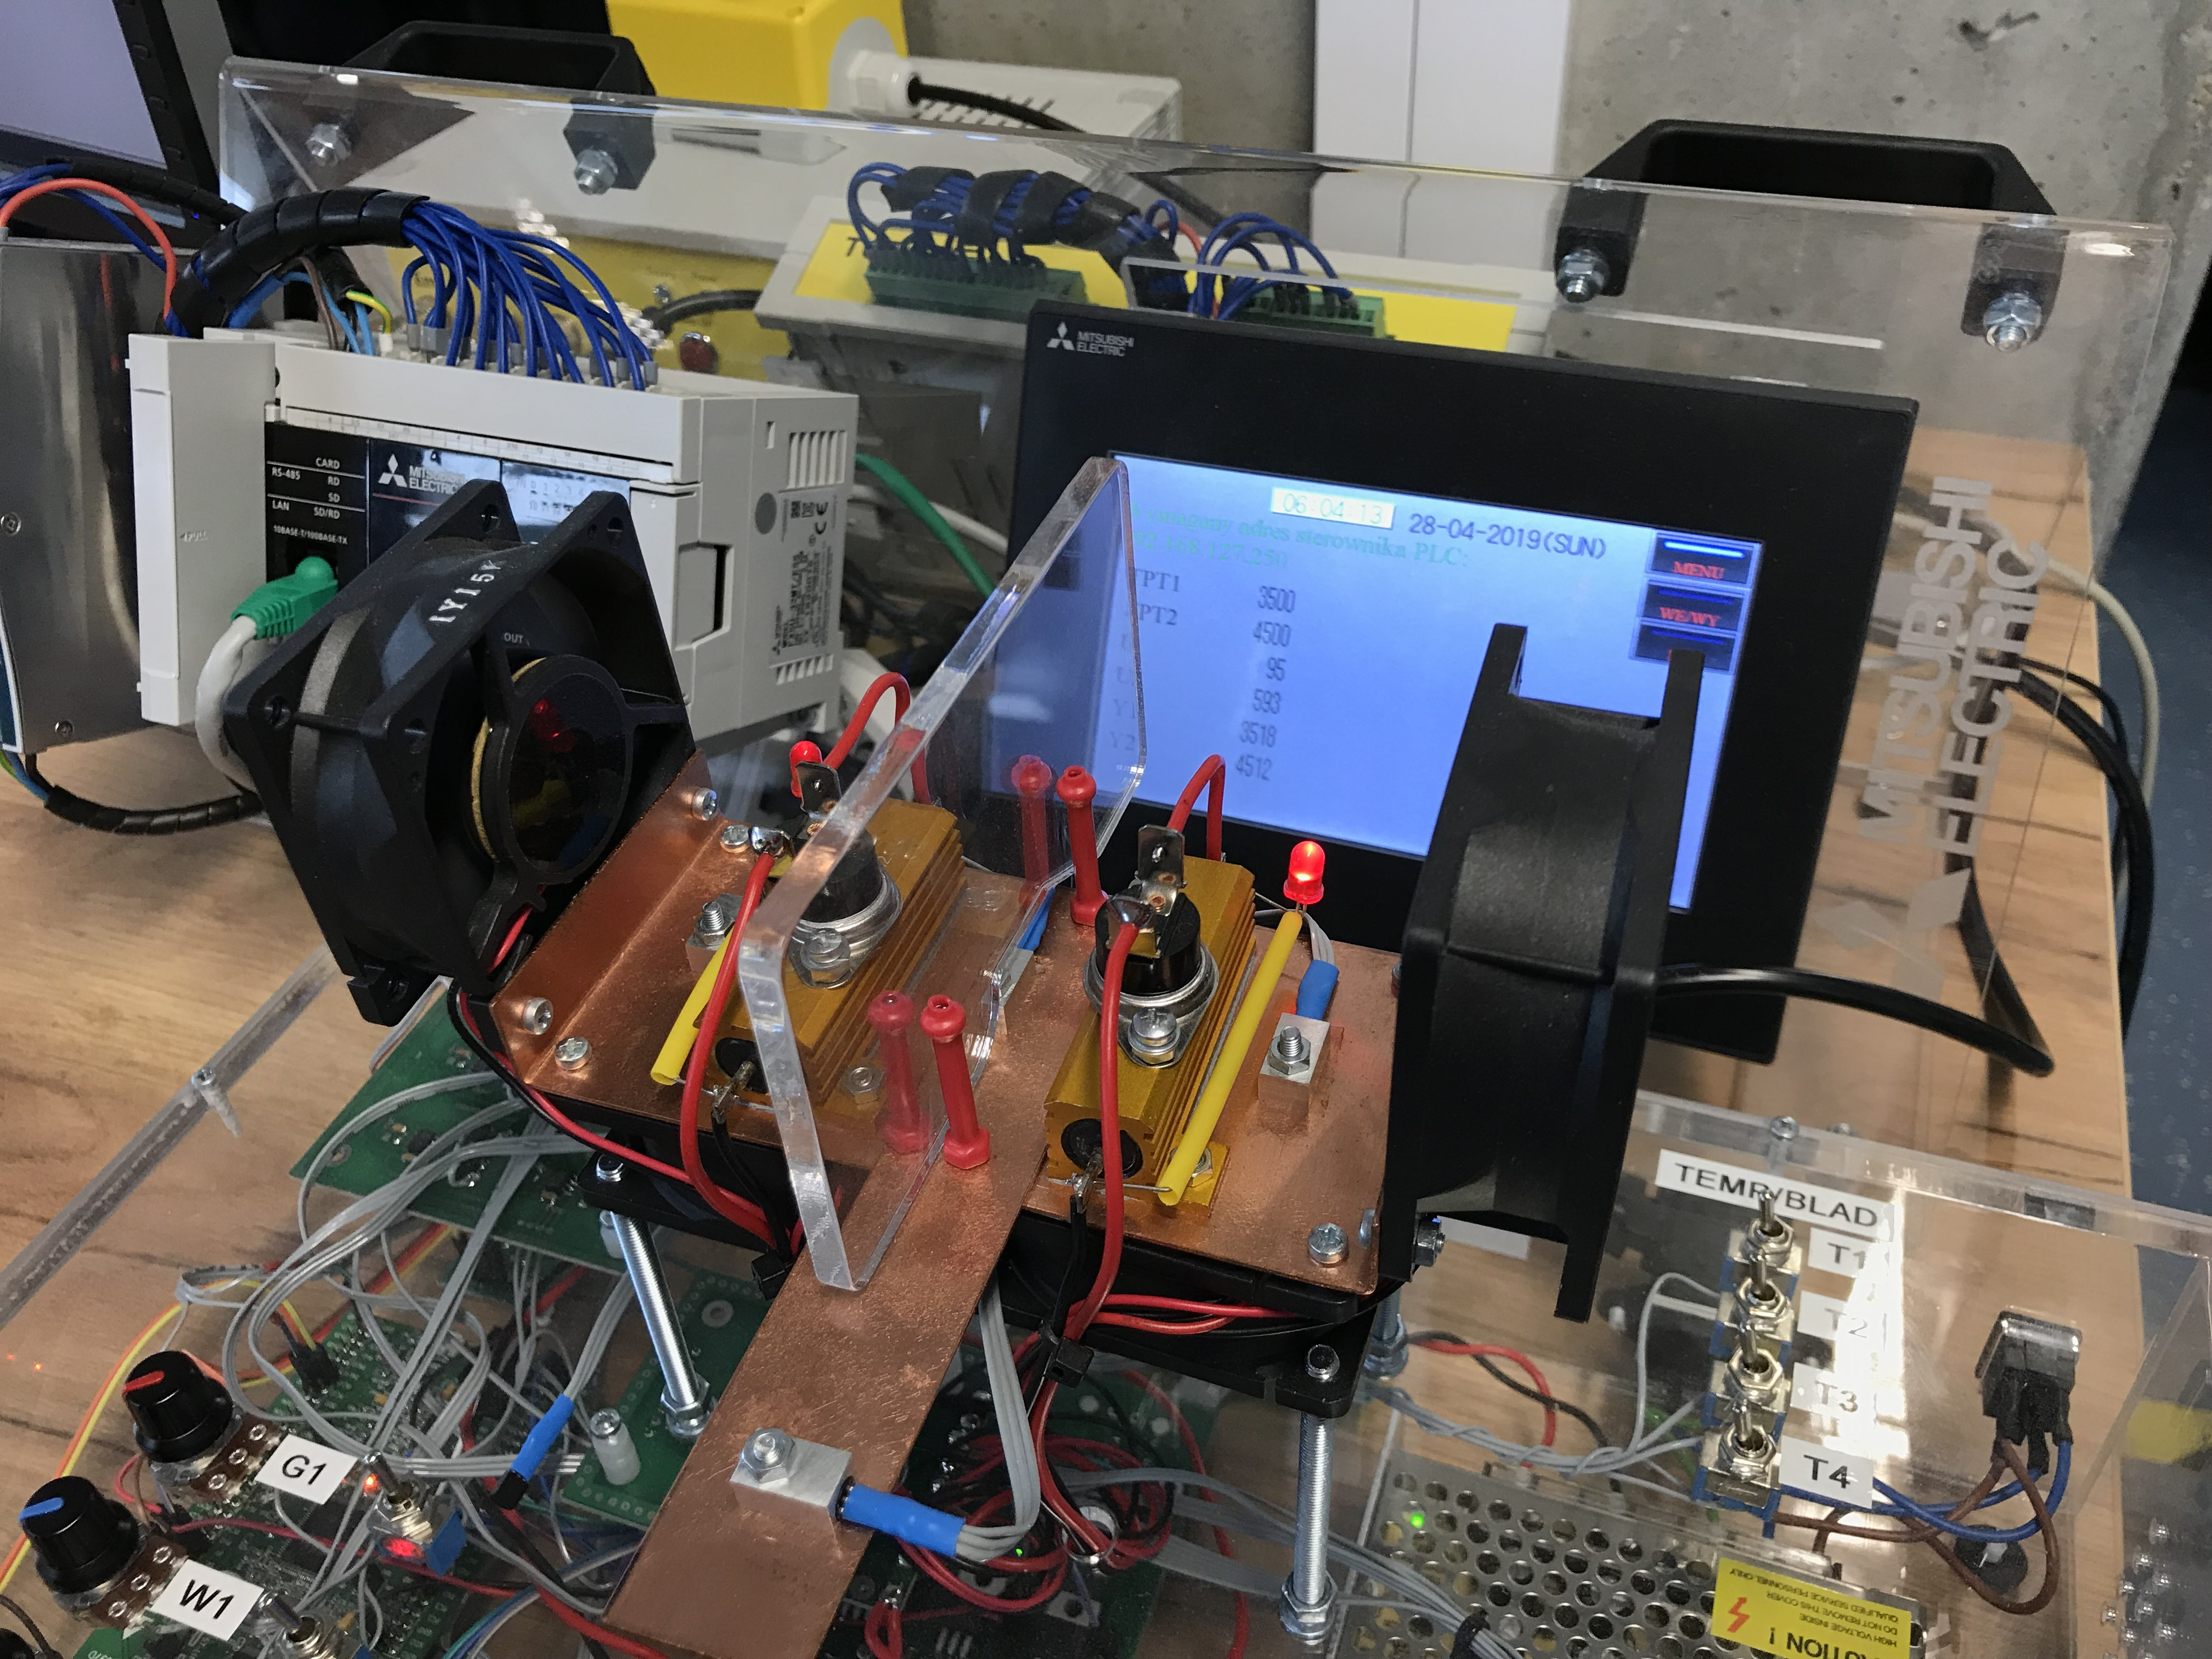
\includegraphics[scale=0.09]{../data/lab/thermal_object/zad5/IMG_0964.JPG}
\caption{Pracujące stanowisko chłodząco-grzejące z działającym w tle panelem operatorskim}
\end{figure}

\begin{figure}[H]
\includegraphics[scale=0.09]{../data/lab/thermal_object/zad5/IMG_0965.JPG}
\caption{Panel operatorski pokazujący aktualne dane z zachodzącego procesu regulacji}
\end{figure}

\begin{figure}[H]
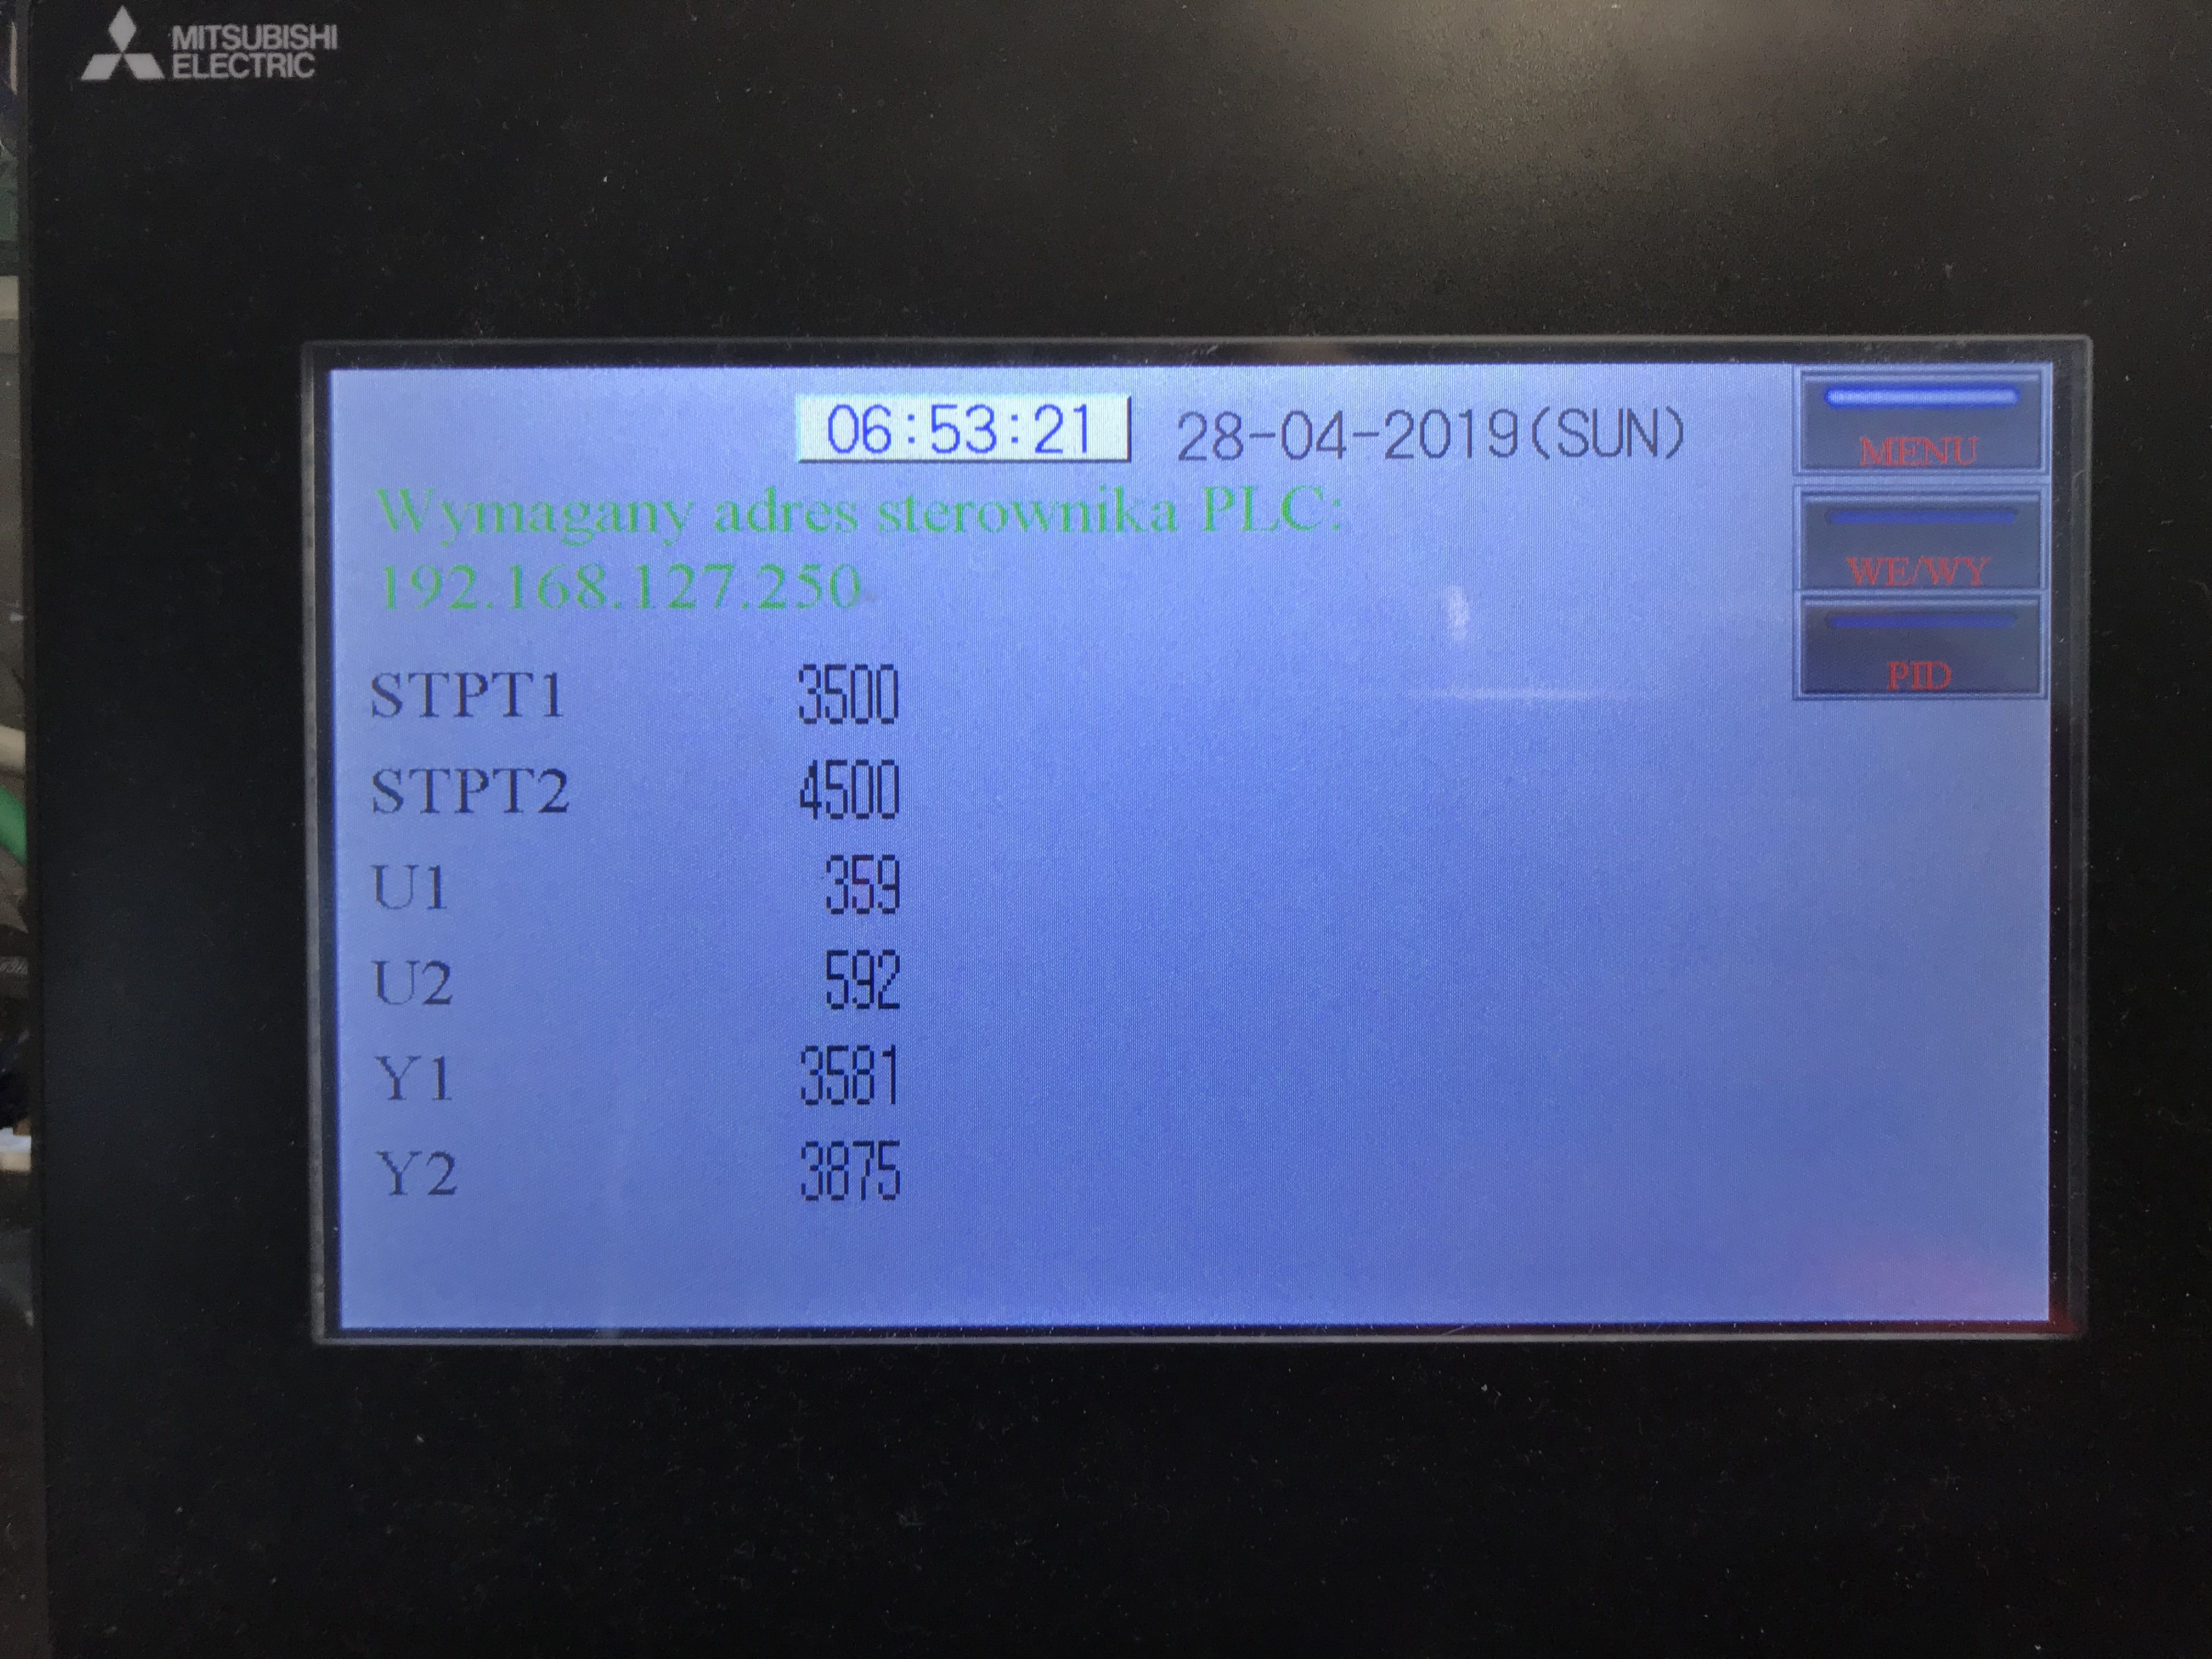
\includegraphics[scale=0.09]{../data/lab/thermal_object/zad5/IMG_0966.JPG}
\caption{Panel operatorski pokazujący aktualne dane z zachodzącego procesu regulacji}
\end{figure}
\chapter{Automat sterujący}
\label{thermal_automat}


\part{Laboratorium - stanowisko INTECO CRANE}
%\chapter{Opis stanowiska INTECO CRANE}
\label{inteco_stanowisko}


%\chapter{Zabezpieczenia stanowiska INTECO CRANE}
\label{inteco_zabezpieczenie}

\section{Procedura bazowania}
\label{homecoming}
\begin{lstlisting}
IF start_homing = TRUE THEN	
  IF homed_X = FALSE THEN
	IF krancowka_X = FALSE THEN
		SET(TRUE, X_enable); 
		RST(TRUE, X_direction);
		MOV(TRUE, K30, X_PWM);
		MOVB(TRUE, TRUE,  X_allowPWM);
	ELSE
		MOV(TRUE, K1, X_PWM);
		RST(TRUE, X_enable);
		DHCMOVP(TRUE, 0, 0, SD4500); 
		MOVB(TRUE, TRUE, homed_X);
	END_IF;
  END_IF;	
  IF homed_Y = FALSE THEN
	IF krancowka_Y = FALSE THEN
		SET(TRUE, Y_enable); 
		RST(TRUE, Y_direction);
		MOV(TRUE, K30, Y_PWM);
		MOVB(TRUE,TRUE,  Y_allowPWM);
	ELSE
		MOV(TRUE, K1, Y_PWM);
		RST(TRUE,  Y_enable);
		DHCMOVP(TRUE, 0, 0, SD4620); 
		MOVB(TRUE, TRUE, homed_Y);
	END_IF;
  END_IF;	
  IF homed_X AND homed_Y THEN
	start_homing := FALSE;
  END_IF;	
END_IF;
\end{lstlisting}


Aby rozpoczynać pracę w położeniu początkowym, zawarliśmy w projekcie procedurę bazującą obiekt. Zadaniem programu było ustawienie obiektu w zerowym położeniu dla obydwu osi. Procedurę rozpoczynało ustawienie flagi \verb+start_homing+. Następnie sprawdzane były warunki na bazowanie osi (flagi \verb+homed_X+, \verb+homed_Y+). Do momentu osiągnięcia stanu wysokiego na czujnikach krańcowych dla każdej osi, odbywał się ruch obiektu w kierunku czujników. Gdy czujniki zostały aktywowane, rejestry przechowujące wartości odczytów z enkoderów były zerowane, co kończyło bazowanie.\\

\section{Program ST}
\label{program_zabezpieczenia}

\begin{lstlisting}
IF homed_X = TRUE THEN
  IF encoder_X > K9450 OR encoder_X < -K50 THEN
	MOVB(TRUE, FALSE, X_enable);
	PWM(FALSE, K1, K100, X_output);
	MOVB(TRUE, FALSE, homed_X);
  END_IF;
END_IF;

IF homed_Y = TRUE THEN
  IF encoder_Y  > K2350 OR encoder_Y < -K50 THEN
	MOVB(TRUE, FALSE, Y_enable);
	PWM(FALSE, K1, K100, Y_output);
	MOVB(TRUE, FALSE, homed_Y);
  END_IF;
END_IF;
\end{lstlisting}

Programowe zabezpieczenia zostały zrealizowane w programie przedstawionym powyżej. W programie pod warunkiem wykrycia wcześniejszego bazowania obiektu, badane były wartości enkoderów odpowiadających poszczególnym osiom. W przypadku przekroczenia maksymalnych wartości dopuszczalnych na którymś z enkoderów, dalszy ruch w danej osi był blokowany poprzez reset flagi \verb+brake+ dla odpowiednich osi. Następnie resetowana była również flaga bazowania blokowanej osi.


\section{Zabezpieczenie sprzętowe}
Każdy obiekt z rodziny INTECO w laboratorium CS402 zawiera czerwony, awaryjny przycisk bezpieczeństwa. Podczas pracy z obiektem TCRANE był on szczególnie potrzebny ponieważ obiekt czasem nie pracował tak jakbyśmy sobie tego życzyli. Podczas eksperymentów trzeba było uważać zarówno na obiekt jak i na osoby w jego otoczeniu. W kryzysowych sytuacjach odłączaliśmy zasilanie od obiektu wciskając przycisk bezpieczeństwa.
\label{czerwony_przycisk}

%\chapter{Wyznaczenie charakterystyki statycznej obiektu}
\label{lab2}

Aby wyznaczyć charakterystykę statyczną wykonaliśmy eksperyment mający na celu zbadanie wzmocnienia w zależności od sterowania. Dla kolejnych wartości sygnału sterującego: $20, 30, 40...$ oczekiwaliśmy stabilizacji sygnału wyjściowego obiektu. Wynik eksperymentu przedstawia wykres \ref{eksperyment}. Na wykresie możemy zauważyć, że przyrost wartości sygnału wyjściowego zmniejsza się wraz ze zwiększaniem wartości sterowania. Punkty stabilizacji sygnału posłużyły do wyznacznia charakterystyki statycznej obiektu. Wynik aproksymacji przedstawia wykrest \ref{char_stat}.\\
\indent{} Przegięcie wykresu wskazuje na to, że mamy do czynienia z obiektem nieliniowym, dlatego niemożliwe jest wyznaczenie jednego wzmocnienia statycznego 
opisującego cały proces.

\begin{figure}[b]
    \centering
    \begin{tikzpicture}
    \begin{axis}[
    width=0.98\textwidth,
    xmin=0.0,xmax=2040,ymin=30,ymax=55,
    xlabel={$k$},
    ylabel={$y[k]$},
    legend pos=south east,
    y tick label style={/pgf/number format/1000 sep=},
    ] 
    \addlegendentry{$y[k]$},
    \addlegendimage{no markers,red}

    \addplot[red, semithick] file{../data/lab/zad2/eksperyment.csv};  
    \end{axis}
    \end{tikzpicture}
    \caption{Przebieg eksperymentu przy wartościach sterowania: $20, 30, 40, 50, 60, 70, 80$}
    \label{eksperyment}
\end{figure}

\begin{figure}[t]
    \centering
    \begin{tikzpicture}
    \begin{axis}[
    width=0.98\textwidth,
    xmin=20.0,xmax=80,ymin=32,ymax=52,
    xlabel={$u$},
    ylabel={$y[u]$},
    legend pos=south east,
    y tick label style={/pgf/number format/1000 sep=},
    ] 
    \addlegendentry{$y[u]$},
    \addlegendimage{no markers,red}

    \addplot[red, semithick] file{../data/lab/zad2/char_stat.csv};  
    \end{axis}
    \end{tikzpicture}
    \caption{Charakterystyka statyczna obiektu}
    \label{char_stat}
\end{figure}
%\chapter{Dobieranie nastawów regulatorów PID}
\label{zad5}

\section{Strojenie regulatora PID}
\label{zad5_PID_wykresy}
W celu dobrania optymalnych parametrów regulatora, wyszliśmy od parametrów uzyskanych metodą
Zieglera-Nicholsa a następnie ręcznie dostroiliśmy poszczególne parametry tak aby uzyskać
jak najlepszy efekty końcowy. Eksperyment ten polegał na znalezieniu takiego wzmocnienia $K_{r}$, 
zwanego wzmocnieniem krytycznym, dla którego obiekt wpadał w niegasnące oscylacje o okresie $T_{k}$. 

Cały proces dobierania parametrów składał się z następujących kroków:
\begin{center}
\begin{enumerate}
    \item Wyznaczenie wzmocnienia $K_{\mathrm{k}}$ i okresu oscylacji $T_{\mathrm{k}}$
    \item Wyliczenie parametrów regulatora
    \item Ręczna poprawa wartości wzmocnienia członu proporcjonalnego $K_{\mathrm{r}}$
    \item Ręczna poprawa wartości parametru członu całkującego $T_{\mathrm{i}}$
    \item Ręczna poprawa wartości parametru członu różniczkującego $T_{\mathrm{d}}$
\end{enumerate}
\end{center}

Chcąc znaleźć jeszcze lepsze nastawy regulatora, po wyznaczeniu parametrów za pomocą metody Zieglera-Nicholsa, zastosowaliśmy metodę eksperymentalną. W której jakość regulacji ocenialiśmy jakościowo (na podstawie przebiegów sygnałów na wykresach) oraz ilościowo, za pomocą wskaźnika jakości regulacji danego wzorem:
\begin{equation}
E=\sum_{k=0}^{K_{konc}}(y^{zad}[k]-y[k])^{2}
\end{equation}


\subsection{Wyznaczenie wzmocnienia $K_{\mathrm{k}}$ i okresu oscylacji $T_{\mathrm{k}}$}
\label{zad5_wyznaczanie_parametrow_zn}
Na początku doprowadziliśmy układ do granicy stabilności, czyli momentu
w którym zaczęły pojawiać się niegasnące oscylacje. Zrealizowaliśmy to
zwiększając współczynnik wzmocnienia $K_{\mathrm{r}}$ przy wyłączonych członach 
całkującym i różniczkującym. Iteracyjnie wyznaczaliśmy nowe wartości wzmocnienia,
zwiększając jego wartość w przypadku gasnących oscylacji oraz zmniejszając w przypadku
niestabilnej odpowiedzi obiektu.

Gdy ostatecznie zaobserwowaliśmy niegasnące oscylacje zapisaliśmy aktualne wzmocnienie 
jako wzmocnienie krytyczne $K_{k}$ i zmierzyliśmy okres oscylacji drgań 
krytycznych $T_{k}$ ($K_{k} = 1,8 \hspace{0.3 cm} T_{k}=18,5 $). Wiedząc że okres próbkowania procesu 
wynosi $\num{0,5}s$, a zmierzony okres oscylacji wynosił $\num{37}$ próbek, wyliczyliśmy że
okres drgań krytycznych równa się $T_{k}=18,5s$. 

\begin{figure}[t]
    \centering
    \begin{tikzpicture}
    \begin{axis}[
    width=0.98\textwidth,
    xmin=0,xmax=500,ymin=3.7, ymax=4.3,
    xlabel={$k$},
    ylabel={$y[k]$},
    %xtick={0, 100, 200, 300, 400, 500},
    %ytick={3.9, 4, 4.1, 4.2, 4.3, 4.4},
    legend pos=south east,
    y tick label style={/pgf/number format/1000 sep=},
    ]
    \addplot[blue, semithick] file{../data/Zad5_figure_data/zad5_PID_setpoint_exampleK_1.8_Ti_1000000000000_Td_0.csv};
    \addplot[red, semithick] file{../data/Zad5_figure_data/zad5_PID_output_exampleK_1.8_Ti_1000000000000_Td_0.csv};
    \addlegendentry{$y^{zad}[k]$},
    \addlegendentry{$y[k]$},
    \addlegendimage{no markers, blue}
	\addlegendimage{no markers, red}
    \end{axis}
    \end{tikzpicture}
    \caption{Niegasnące oscylacje wyjścia obiektu przy wzmocnieniu krytycznym}
    \label{zad5_niegasnace_oscylacje}
\end{figure}

\begin{figure}[b]
    \centering
    \begin{tikzpicture}
    \begin{axis}[
    width=0.98\textwidth,
    xmin=0,xmax=500,ymin=0.25, ymax=0.75,
    xlabel={$k$},
    ylabel={$u[k]$},
    %xtick={0, 0.4, 0.5, 0.6, 0.7},
    %ytick={3.5, 3.75, 4, 4.25, 4.5},
    legend pos=south east,
    y tick label style={/pgf/number format/1000 sep=},
    ]
    \addplot[const plot, blue, semithick] file{../data/Zad5_figure_data/zad5_PID_input_exampleK_1.8_Ti_1000000000000_Td_0.csv};
    \legend{$u[k]$}
    \end{axis}
    \end{tikzpicture}
    \caption{Przebieg sygnału sterującego }
    \label{zad5_niegasnace_oscylacje_ster}
\end{figure}
\FloatBarrier

\subsection{Wyliczenie wstępnych parametrów regulatora}
\label{zad5_regulator_zn}
Dobierając nastawy według metody Zieglera-Nicholsa, 
stosowaliśmy wzory do obliczenia parametrów regulatora PID: 

\begin{equation}
\label{zad5_zn_wzory}
K_{\mathrm{r}}=\num{0,6}K_{\mathrm{k}} \hspace{1cm} T_{\mathrm{i}}=\num{0,5} \hspace{1cm} T_{\mathrm{k}} T_{\mathrm{d}}=\num{0,12} T_{\mathrm{k}}
\end{equation}
gdzie:
\begin{center}
\begin{itemize}
    \item $K_{\mathrm{k}}$ - wzmocnienie krytyczne
    \item $T_{\mathrm{k}}$ - okres oscylacji
\end{itemize}
\end{center}

Wyliczone wartości liczbowe parametrów:
\begin{center}
$K_{r}=\num{1,08} \hspace{0.5 cm}
T_{i}=\num{9,25}   \hspace{0.5 cm}
T_{d}=\num{2,22}$
\end{center}

Regulator z parametrami wyznaczonymi przy pomocy metody opisanej przez panów Johna Zieglera
i Nathaniela Nicholsa, nadal charakteryzuje się niegasnącymi oscylacjami. Takie 
przebiegi sygnałów są nieakceptowalne, dlatego w dalszych krokach ręcznie modyfikowaliśmy 
wartości parametrów. 

Na rysunku \ref{zad5_zn_regulator} przedstawiono przebiegu wartości zadanej oraz
wyjścia obiektu z widocznie przedstawionymi oscylacjami wokół wartości zadanej.
Rysunek \ref{zad5_zn_sterowanie} przedstawia zmianę sygnału sterującego
generowanego przez regulator.

Tak nastrojony regulator PID bardzo słabo radzi sobie z utrzymywaniem sygnału wyjściowego
procesu na poziomie wartości zadanej. Niegasnące oscylacje nie pozwalają na zastosowanie
tego zestawu parametrów do regulacji procesem. Dla zadanej trajektorii testowej, obliczony 
wskaźnik jakości regulacji wyniósł $E = \num{5,8385}$. Pomimo swoich wad, regulator ten jest 
dobrym punktem wyjścia dla metody eksperymentalnej.

\begin{figure}[t]
    \centering
    \begin{tikzpicture}
    \begin{axis}[
    width=0.98\textwidth,
    xmin=0,xmax=600,ymin=3.7, ymax=4.4,
    xlabel={$k$},
    ylabel={$y[k]$},
    %xtick={0.3, 0.4, 0.5, 0.6, 0.7},
    %ytick={3.5, 3.75, 4, 4.25, 4.5},
    legend pos=south east,
    y tick label style={/pgf/number format/1000 sep=},
    ]
    \addplot[blue, semithick] file{../data/zad5_multiplejumps/zad5_PID_setpoint_exampleK_1.08_Ti_9.25_Td_2.22_E_5.8385.csv};
    \addplot[red, semithick] file{../data/zad5_multiplejumps/zad5_PID_output_exampleK_1.08_Ti_9.25_Td_2.22_E_5.8385.csv};
    \addlegendentry{$y^{zad}[k]$},
    \addlegendentry{$y[k]$},
    \addlegendimage{no markers, blue}
	\addlegendimage{no markers, red}
    \end{axis}
    \end{tikzpicture}
    \caption{Przebieg procesu sterowanego za pomocą regulatora z parametrami wyznaczonymi za pomocą metody Zieglera-Nicholsa}
    \label{zad5_zn_regulator}
\end{figure}

\begin{figure}[b]
    \centering
    \begin{tikzpicture}
    \begin{axis}[
    width=0.98\textwidth,
    xmin=0.0,ymin=0.3, xmax= 600,
    xlabel={$k$},
    ylabel={$u[k]$},
    %xtick={0.3, 0.4, 0.5, 0.6, 0.7},
    %ytick={3.5, 3.75, 4, 4.25, 4.5},
    legend pos=south east,
    y tick label style={/pgf/number format/1000 sep=},
    ]
    \addplot[const plot, blue, semithick] file{../data/zad5_multiplejumps/zad5_PID_input_exampleK_1.08_Ti_9.25_Td_2.22_E_5.8385.csv};
    \legend{$u[k]$}
    \end{axis}
    \end{tikzpicture}
    \caption{Przebieg sygnału sterującego regulatora z parametrami wyznaczonymi za pomocą metody Zieglera-Nicholsa}
    \label{zad5_zn_sterowanie}
\end{figure}
\FloatBarrier

\subsection{Ręczna poprawa wartości wzmocnienia członu proporcjonalnego $K_{\mathrm{r}}$ }
\label{zad5_poprawa_Kr}
\subsubsection{Wzmocnienie regulatora $\mathbf{K_{\mathrm{r}}}=\num{0,75}$}
W pierwszej kolejności skupiliśmy się na zmianie parametru $K_{\mathrm{r}}$.
Zmniejszenie $K_{\mathrm{r}}$ do wartości $\num{0.75}$ sprawiło że pozbyliśmy się oscylacji. Czas regulacji
wyniósł około 100 próbek. Dodatkowo, sygnał wyjściowy procesu nie cechuje się przeregulowaniem,
czyli przekroczenie wartości zadanej. Wyjście obiektu już nie oscyluje tak jak to było w przypadku regulatora z \ref{zad5_regulator_zn},
jak i została przywrócona stabilność procesu. Sygnał sterujący cechuje się oscylacjami przy zmianach
wartości zadanej, co powoduje nierówny przebieg wyjścia procesu.
Wartość wskaźnika jakości regulacji dla tego regulatora przy tej samej
testowej trajektorii zadanej wyniosła $E=\num{5,6914}$, co jest niewielką poprawą w stosunku 
do bazowego regulatora.
Przebiegi sygnału wyjściowego jaki i sygnału sterującego, odbiegały od pożądanych.

Wykres \ref{zad5_1_K_odp} przedstawia przebiegi wyjścia procesu oraz trajektorii zadanej.
Na rysunku \ref{zad5_1_zmiana_K} przedstawiliśmy przebieg sygnału sterującego generowanego przez regulator.

\subsubsection{Wzmocnienie regulatora $\mathbf{K_{\mathrm{r}}}=\num{0,6}$}
Zmniejszenie $K_{\mathrm{r}}$ do poziomu $\num{0,6}$ spowodowało wizualną poprawę odpowiedzi układu 
na zmianę wartości zadanej. Przebieg sygnału wyjściowego wygładził się, proces w łagodniejszy sposób
dociera do wartości zadanej. Czas regulacji niie zmienił się w porównaniu do poprzedniego regulatora.
Przebieg sygnału sterującego również uległ wygładzeniu, chociaż oscylacje nie zniknęły w całości.
Wartość wskaźnika jakości regulacji dla tego 
przypadku wyniosła $E=\num{6.1449}$, co zaskakująco, jest wartością większą w porównaniu do poprzedniego 
$K_{\mathrm{r}}$ regulatora. Łagodniejszy przebieg wyjścia powoduje zwiększenie sumy kwadratów uchybu.

Wykres \ref{zad5_2_K_odp} przedstawia przebiegi wyjścia procesu oraz trajektorii zadanej.
Na rysunku \ref{zad5_2_zmiana_K} przedstawiliśmy przebieg sygnału sterującego generowanego przez regulator.

\subsubsection{Wzmocnienie regulatora $\mathbf{K_{\mathrm{r}}}=\num{0,5}$}
Na wykresach \ref{zad5_3_K_odp} i \ref{zad5_3_zmiana_K} przedstawiono przebiegi powstałe 
dla regulatora z wzmocnieniem $ K_{\mathrm{r}} = \num{0,5}$. Sygnał sterujący praktycznie nie
oscyluje, natomiast sygnał wyjściowy ma jeszcze łagodniejszy przebieg co niestety sprawia że czas regulacji 
nieznacznie wzrósł. Niestety, wskaźnik jakości 
regulacji wzrósł do wartości $E=\num{6,5814}$. Zauważyliśmy, że jego wartość rośnie przy zmniejszaniu  
parametru $ K_{\mathrm{r}}$, dlatego postanowiliśmy 
ostatecznie przyjąć wartość $K_{\mathrm{r}} = \num{0,5}$ i przejść do manipulowania 
pozostałymi parametrami. Dalsze zmniejszanie nie spowoduje 
znaczącej poprawy przebiegów a jedynie pogorszy wskaźnik jakości regulacji. 

%%%%%%%%%%%%%%%%%%%%%%%%%%%%% wykresy dla k = 0.75

\begin{figure}[t]
    \centering
    \begin{tikzpicture}
    \begin{axis}[
    width=0.98\textwidth,
    xmin=0,xmax=600,ymin=3.8, ymax=4.4,
    xlabel={$k$},
    ylabel={$y[k]$},
    %xtick={0.3, 0.4, 0.5, 0.6, 0.7},
    %ytick={3.5, 3.75, 4, 4.25, 4.5},
    legend pos=south east,
    y tick label style={/pgf/number format/1000 sep=},
    ]
    \addplot[blue, semithick] file{../data/zad5_multiplejumps/P/zad5_PID_setpoint_exampleK_0.75_Ti_9.25_Td_2.22_E_5.6914.csv};
    \addplot[red, semithick] file{../data/zad5_multiplejumps/P/zad5_PID_output_exampleK_0.75_Ti_9.25_Td_2.22_E_5.6914.csv};
    \addlegendentry{$y^{zad}[k]$},
    \addlegendentry{$y[k]$},
    \addlegendimage{no markers, blue}
	\addlegendimage{no markers, red}
    \end{axis}
    \end{tikzpicture}
    \caption{Przebieg procesu sterowanego za pomocą regulatora z 
    parametrami \mbox{$K_{\mathrm{r}} = \num{0,75}$; $T_{\mathrm{i}} = \num{9,25}$; $T_{\mathrm{d}} = \num{2,22}$}}
    \label{zad5_1_K_odp}
\end{figure}

\begin{figure}[b]
    \centering
    \begin{tikzpicture}
    \begin{axis}[
    width=0.98\textwidth,
    xmin=0.0, ymin=0.44, xmax=600, ymax=0.68,
    xlabel={$k$},
    ylabel={$u[k]$},
    %xtick={0.3, 0.4, 0.5, 0.6, 0.7},
    %ytick={3.5, 3.75, 4, 4.25, 4.5},
    legend pos=south east,
    y tick label style={/pgf/number format/1000 sep=},
    ]
    \addplot[const plot, blue, semithick] file{../data/zad5_multiplejumps/P/zad5_PID_input_exampleK_0.75_Ti_9.25_Td_2.22_E_5.6914.csv};
    \legend{$u[k]$}
    \end{axis}
    \end{tikzpicture}
    \caption{Przebieg sygnału sterującego generowanego przez regulator z 
    parametrami \mbox{$K_{\mathrm{r}} = \num{0,75}$; $T_{\mathrm{i}} = \num{9,25}$; $T_{\mathrm{d}} = \num{2,22}$}}
    \label{zad5_1_zmiana_K}
\end{figure}
\FloatBarrier

%%%%%%%%%%%%%%%%%%%%%%%%%%%%% wykresy dla k = 0.6


\begin{figure}[t]
    \centering
    \begin{tikzpicture}
    \begin{axis}[
    width=0.98\textwidth,
    xmin=0,xmax=600,ymin=3.8, ymax=4.4,
    xlabel={$k$},
    ylabel={$y[k]$},
    %xtick={0.3, 0.4, 0.5, 0.6, 0.7},
    %ytick={3.5, 3.75, 4, 4.25, 4.5},
    legend pos=south east,
    y tick label style={/pgf/number format/1000 sep=},
    ]
    \addplot[blue, semithick] file{../data/zad5_multiplejumps/P/zad5_PID_setpoint_exampleK_0.6_Ti_9.25_Td_2.22_E_6.1449.csv};
    \addplot[red, semithick] file{../data/zad5_multiplejumps/P/zad5_PID_output_exampleK_0.6_Ti_9.25_Td_2.22_E_6.1449.csv};
    \addlegendentry{$y^{zad}[k]$},
    \addlegendentry{$y[k]$},
    \addlegendimage{no markers, blue}
	\addlegendimage{no markers, red}
    \end{axis}
    \end{tikzpicture}
    \caption{Przebieg procesu sterowanego za pomocą regulatora z 
    parametrami \mbox{$K_{\mathrm{r}} = \num{0,6}$; $T_{\mathrm{i}} = \num{9,25}$; $T_{\mathrm{d}} = \num{2,22}$}}
    \label{zad5_2_K_odp}
\end{figure}

\begin{figure}[b]
    \centering
    \begin{tikzpicture}
    \begin{axis}[
    width=0.98\textwidth,
    xmin=0.0,ymin=0.44, xmax=600, ymax=0.68,
    xlabel={$k$},
    ylabel={$u[k]$},
    %xtick={0.3, 0.4, 0.5, 0.6, 0.7},
    %ytick={3.5, 3.75, 4, 4.25, 4.5},
    legend pos=south east,
    y tick label style={/pgf/number format/1000 sep=},
    ]
    \addplot[const plot, blue, semithick] file{../data/zad5_multiplejumps/P/zad5_PID_input_exampleK_0.6_Ti_9.25_Td_2.22_E_6.1449.csv};
    \legend{$u[k]$}
    \end{axis}
    \end{tikzpicture}
    \caption{Przebieg sygnału sterującego generowanego przez regulator z 
    parametrami \mbox{$K_{\mathrm{r}} = \num{0,6}$; $T_{\mathrm{i}} = \num{9,25}$; $T_{\mathrm{d}} = \num{2,22}$}}
    \label{zad5_2_zmiana_K}
\end{figure}
\FloatBarrier

%%%%%%%%%%%%%%%%%%%%%% wykresy dla k = 0.5

\begin{figure}[t]
    \centering
    \begin{tikzpicture}
    \begin{axis}[
    width=0.98\textwidth,
    xmin=0,xmax=600, ymin=3.8, ymax=4.4,
    xlabel={$k$},
    ylabel={$y[k]$},
    %xtick={0.3, 0.4, 0.5, 0.6, 0.7},
    %ytick={3.5, 3.75, 4, 4.25, 4.5},
    legend pos=south east,
    y tick label style={/pgf/number format/1000 sep=},
    ]
    \addplot[blue, semithick] file{../data/zad5_multiplejumps/P/zad5_PID_setpoint_exampleK_0.5_Ti_9.25_Td_2.22_E_6.5814.csv};
    \addplot[red, semithick] file{../data/zad5_multiplejumps/P/zad5_PID_output_exampleK_0.5_Ti_9.25_Td_2.22_E_6.5814.csv};
    \addlegendentry{$y^{zad}[k]$},
    \addlegendentry{$y[k]$},
    \addlegendimage{no markers, blue}
	\addlegendimage{no markers, red}
    \end{axis}
    \end{tikzpicture}
    \caption{Przebieg procesu sterowanego za pomocą regulatora z 
    parametrami \mbox{$K_{\mathrm{r}} = \num{0,5}$; $T_{\mathrm{i}} = \num{9,25}$; $T_{\mathrm{d}} = \num{2,22}$}}
    \label{zad5_3_K_odp}
\end{figure}

\begin{figure}[b]
    \centering
    \begin{tikzpicture}
    \begin{axis}[
    width=0.98\textwidth,
    xmin=0.0,ymin=0.44, xmax=600, ymax=0.68,
    xlabel={$k$},
    ylabel={$u[k]$},
    %xtick={0.3, 0.4, 0.5, 0.6, 0.7},
    %ytick={3.5, 3.75, 4, 4.25, 4.5},
    legend pos=south east,
    y tick label style={/pgf/number format/1000 sep=},
    ]
    \addplot[const plot, blue, semithick] file{../data/zad5_multiplejumps/P/zad5_PID_input_exampleK_0.5_Ti_9.25_Td_2.22_E_6.5814.csv};
    \legend{$u[k]$}
    \end{axis}
    \end{tikzpicture}
    \caption{Przebieg sygnału sterującego generowanego przez regulator z 
    parametrami \mbox{$K_{\mathrm{r}} = \num{0,5}$; $T_{\mathrm{i}} = \num{9,25}$; $T_{\mathrm{d}} = \num{2,22}$}}
    \label{zad5_3_zmiana_K}
\end{figure}
\FloatBarrier

\subsection{Ręczna poprawa wartości czasu zdwojenia $T_{\mathrm{i}}$ }
\label{zad5_poprawa_Ti}

\subsubsection{Czas zdwojenia regulatora $\mathbf{T_{\mathrm{i}}}=\num{8,25}$}
W pierwszej kolejności postanowiliśmy minimalnie zmniejszyć wartość czasu zdwojenia
aby sprawdzić jak niewielkie zmiany tego parametru wpływają na końcowe przebiegi.
Okazuje się że zmniejszenie parametru $\mathbf{T_{\mathrm{i}}}=\num{8,25}$, bardzo
pozytywnie wpływa na przebiegi sygnałów wejściowego i wyjściowego. Nie występuje przeregulowanie
a czas regulacji został skrócony. Wartość wskaźnika jakości równa jest $E = \num{6,1901}$, co jest poprawą
w stosunku do poprzednio omawianego regulatora.

Przebiegi sygnału wyjściowego z zaznaczoną trajektorią zadaną oraz sygnału wejściowego znajdują się 
odpowiednio na rysunkach \ref{zad5_1_Ti_odp} i \ref{zad5_1_zmiana_Ti}.

\subsubsection{Czas zdwojenia regulatora $\mathbf{T_{\mathrm{i}}}=\num{7,25}$}
Idąc drogą obraną przy pierwszym regulatorze, postanowiliśmy jeszcze bardziej zmniejszyć 
czas zdwojenia $T_{\mathrm{i}}$. W kolejnej iteracji obraliśmy wartość parametru
$T_{\mathrm{i}}=\num{7,25}$. Zastosowanie takiej wartości spowodowało że przebieg 
sygnału wyjściowego jeszcze szybciej zbiegł do wartości zadanej. Większy wpływ członu całkującego
sprawia że regulator agresywniej podąża za trajektorią zadaną co objawia się pojawieniem 
niewielkiego przeregulowania i zwiększoną zrywnością sygnału sterującego. Nasze jakościowe 
rozważania potwierdza wskaźnik jakości regulacji którego wartość dla tego eksperymentu
wyniósł $E=\num{5,8298}$ co jest znacząco lepszym wynikiem niż przy $T_{\mathrm{i}}=\num{8,25}$.

Przebieg wyjścia procesu w porównaniu do wartości zadanej znajduje się na rysunku \ref{zad5_2_Ti_odp}.
Wyjście omawianego regulatora znajduje się na wykresie przedstawionym na rysunku \ref{zad5_2_zmiana_Ti}. 

\subsubsection{Czas zdwojenia regulatora $\mathbf{T_{\mathrm{i}}}=\num{6,25}$}
Kontynuując rozważania na temat czasu zdwojenia, zdecydowaliśmy się na jeszcze większe zmniejszenie 
parametru $T_{\mathrm{i}}$. Tym razem wybraliśmy wartość $T_{\mathrm{i}}=\num{6,25}$. Przebieg 
wyjścia procesu charakteryzuje się delikatnym przeregulowaniem, jednak dzięki temu udało się
jeszcze bardziej zredukować czas regulacji. Sygnał sterujący jest charakteryzuje się
większą agresywnością, co objawia się poprzez duże piki przy zmianie wartości zadanej.
Mimo wizualnie gorzej wyglądającego przebiegu wyjścia, wskaźnik jakości regulacji osiągnął najmniejszą
wartość $E=\num{5,5257}$. Przebieg wyjścia obiektu znajduje się na wykresie \ref{zad5_3_Ti_odp}. 
Przebieg sygnału sterującego znajduje się na rysunku \ref{zad5_3_zmiana_Ti}.

\subsubsection{Czas zdwojenia regulatora $\mathbf{T_{\mathrm{i}}}=\num{5,25}$}
Kolejną próbę wykonaliśmy dla regulatora z czasem zdwojenia $T_{\mathrm{i}}=\num{5,25}$. Pomimo
jeszcze lepszej wartości wskaźnika regulacji $E=\num{5,3567}$, to przebiegi sygnału wyjściowego i wejściowego
powodują że musimy odrzucić ten regulator. Bardzo duża zrywność regulatora powoduje że 
sygnał sterujący nasyca się na górnych ograniczeniach przy większych skokach wartości zadanej. Co więcej,
wyjście obiektu cechuje się zwiększonym przeregulowaniem i porównywalnym czasem regulacji. Omawiane przebiegi
znajdują się na rysunkach \ref{zad5_4_Ti_odp} i \ref{zad5_4_zmiana_Ti}. 

Biorąc pod uwagę powyższe rozważania, zdecydowaliśmy się na pozostanie przy wartości parametru $T_{\mathrm{i}} = \num{7,25}$.
Minimalnie przeregulowanie postaramy się zniwelować za pomocą parametru $T_{\mathrm{d}}$. 

%%%%%%%%%%% Ti = 8.25

\begin{figure}[t]
    \centering
    \begin{tikzpicture}
    \begin{axis}[
    width=0.98\textwidth,
    xmin=0,xmax=600, ymin=3.8, ymax=4.4,
    xlabel={$k$},
    ylabel={$y[k]$},
    %xtick={0.3, 0.4, 0.5, 0.6, 0.7},
    %ytick={3.5, 3.75, 4, 4.25, 4.5},
    legend pos=south east,
    y tick label style={/pgf/number format/1000 sep=},
    ]
    \addplot[blue, semithick] file{../data/zad5_multiplejumps/I/zad5_PID_setpoint_exampleK_0.5_Ti_8.25_Td_2.22_E_6.1901.csv};
    \addplot[red, semithick] file{../data/zad5_multiplejumps/I/zad5_PID_output_exampleK_0.5_Ti_8.25_Td_2.22_E_6.1901.csv};
    \addlegendentry{$y^{zad}[k]$},
    \addlegendentry{$y[k]$},
    \addlegendimage{no markers, blue}
	\addlegendimage{no markers, red}
    \end{axis}
    \end{tikzpicture}
    \caption{Przebieg procesu sterowanego za pomocą regulatora z 
    parametrami \mbox{$K_{\mathrm{r}} = \num{0,5}$; $T_{\mathrm{i}} = \num{8,25}$; $T_{\mathrm{d}} = \num{2,22}$}}
    \label{zad5_1_Ti_odp}
\end{figure}

\begin{figure}[b]
    \centering
    \begin{tikzpicture}
    \begin{axis}[
    width=0.98\textwidth,
    xmin=0.0,ymin=0.44, xmax=600, ymax=0.68,
    xlabel={$k$},
    ylabel={$u[k]$},
    %xtick={0.3, 0.4, 0.5, 0.6, 0.7},
    %ytick={3.5, 3.75, 4, 4.25, 4.5},
    legend pos=south east,
    y tick label style={/pgf/number format/1000 sep=},
    ]
    \addplot[const plot, blue, semithick] file{../data/zad5_multiplejumps/I/zad5_PID_input_exampleK_0.5_Ti_8.25_Td_2.22_E_6.1901.csv};
    \legend{$u[k]$}
    \end{axis}
    \end{tikzpicture}
    \caption{Przebieg sygnału sterującego generowanego przez regulator z 
    parametrami \mbox{$K_{\mathrm{r}} = \num{0,5}$; $T_{\mathrm{i}} = \num{8,25}$; $T_{\mathrm{d}} = \num{2,22}$}}
    \label{zad5_1_zmiana_Ti}
\end{figure}


%%%%%%%%%%% Ti = 7.25


\begin{figure}[t]
    \centering
    \begin{tikzpicture}
    \begin{axis}[
    width=0.98\textwidth,
    xmin=0,xmax=600, ymin=3.8, ymax=4.4,
    xlabel={$k$},
    ylabel={$y[k]$},
    %xtick={0.3, 0.4, 0.5, 0.6, 0.7},
    %ytick={3.5, 3.75, 4, 4.25, 4.5},
    legend pos=south east,
    y tick label style={/pgf/number format/1000 sep=},
    ]
    \addplot[blue, semithick] file{../data/zad5_multiplejumps/I/zad5_PID_setpoint_exampleK_0.5_Ti_7.25_Td_2.22_E_5.8298.csv};
    \addplot[red, semithick] file{../data/zad5_multiplejumps/I/zad5_PID_output_exampleK_0.5_Ti_7.25_Td_2.22_E_5.8298.csv};
    \addlegendentry{$y^{zad}[k]$},
    \addlegendentry{$y[k]$},
    \addlegendimage{no markers, blue}
	\addlegendimage{no markers, red}
    \end{axis}
    \end{tikzpicture}
    \caption{Przebieg procesu sterowanego za pomocą regulatora z 
    parametrami \mbox{$K_{\mathrm{r}} = \num{0,5}$; $T_{\mathrm{i}} = \num{7,25}$; $T_{\mathrm{d}} = \num{2,22}$}}
    \label{zad5_2_Ti_odp}
\end{figure}

\begin{figure}[b]
    \centering
    \begin{tikzpicture}
    \begin{axis}[
    width=0.98\textwidth,
    xmin=0.0,ymin=0.44, xmax=600, ymax=0.68,
    xlabel={$k$},
    ylabel={$u[k]$},
    %xtick={0.3, 0.4, 0.5, 0.6, 0.7},
    %ytick={3.5, 3.75, 4, 4.25, 4.5},
    legend pos=south east,
    y tick label style={/pgf/number format/1000 sep=},
    ]
    \addplot[const plot, blue, semithick] file{../data/zad5_multiplejumps/I/zad5_PID_input_exampleK_0.5_Ti_7.25_Td_2.22_E_5.8298.csv};
    \legend{$u[k]$}
    \end{axis}
    \end{tikzpicture}
    \caption{Przebieg sygnału sterującego generowanego przez regulator z 
    parametrami \mbox{$K_{\mathrm{r}} = \num{0,5}$; $T_{\mathrm{i}} = \num{7,25}$; $T_{\mathrm{d}} = \num{2,22}$}}
    \label{zad5_2_zmiana_Ti}
\end{figure}
\FloatBarrier


%%%%%%%%%%%% Ti = 6.25


\begin{figure}[t]
    \centering
    \begin{tikzpicture}
    \begin{axis}[
    width=0.98\textwidth,
    xmin=0,xmax=600, ymin=3.8, ymax=4.4,
    xlabel={$k$},
    ylabel={$y[k]$},
    %xtick={0.3, 0.4, 0.5, 0.6, 0.7},
    %ytick={3.5, 3.75, 4, 4.25, 4.5},
    legend pos=south east,
    y tick label style={/pgf/number format/1000 sep=},
    ]
    \addplot[blue, semithick] file{../data/zad5_multiplejumps/I/zad5_PID_setpoint_exampleK_0.5_Ti_6.25_Td_2.22_E_5.5257.csv};
    \addplot[red, semithick] file{../data/zad5_multiplejumps/I/zad5_PID_output_exampleK_0.5_Ti_6.25_Td_2.22_E_5.5257.csv};
    \addlegendentry{$y^{zad}[k]$},
    \addlegendentry{$y[k]$},
    \addlegendimage{no markers, blue}
	\addlegendimage{no markers, red}
    \end{axis}
    \end{tikzpicture}
    \caption{Przebieg procesu sterowanego za pomocą regulatora z 
    parametrami \mbox{$K_{\mathrm{r}} = \num{0,5}$; $T_{\mathrm{i}} = \num{6,25}$; $T_{\mathrm{d}} = \num{2,22}$}}
    \label{zad5_3_Ti_odp}
\end{figure}

\begin{figure}[b]
    \centering
    \begin{tikzpicture}
    \begin{axis}[
    width=0.98\textwidth,
    xmin=0.0,ymin=0.42, xmax=600, ymax=0.7,
    xlabel={$k$},
    ylabel={$u[k]$},
    %xtick={0.3, 0.4, 0.5, 0.6, 0.7},
    %ytick={3.5, 3.75, 4, 4.25, 4.5},
    legend pos=south east,
    y tick label style={/pgf/number format/1000 sep=},
    ]
    \addplot[const plot, blue, semithick] file{../data/zad5_multiplejumps/I/zad5_PID_input_exampleK_0.5_Ti_6.25_Td_2.22_E_5.5257.csv};
    \legend{$u[k]$}
    \end{axis}
    \end{tikzpicture}
    \caption{Przebieg sygnału sterującego generowanego przez regulator z 
    parametrami \mbox{$K_{\mathrm{r}} = \num{0,5}$; $T_{\mathrm{i}} = \num{6,25}$; $T_{\mathrm{d}} = \num{2,22}$}}
    \label{zad5_3_zmiana_Ti}
\end{figure}
\FloatBarrier

%%%%%%%%%%%%% Ti = 5.25


\begin{figure}[t]
    \centering
    \begin{tikzpicture}
    \begin{axis}[
    width=0.98\textwidth,
    xmin=0,xmax=600, ymin=3.8, ymax=4.4,
    xlabel={$k$},
    ylabel={$y[k]$},
    %xtick={0.3, 0.4, 0.5, 0.6, 0.7},
    %ytick={3.5, 3.75, 4, 4.25, 4.5},
    legend pos=south east,
    y tick label style={/pgf/number format/1000 sep=},
    ]
    \addplot[blue, semithick] file{../data/zad5_multiplejumps/I/zad5_PID_setpoint_exampleK_0.5_Ti_5.25_Td_2.22_E_5.3567.csv};
    \addplot[red, semithick] file{../data/zad5_multiplejumps/I/zad5_PID_output_exampleK_0.5_Ti_5.25_Td_2.22_E_5.3567.csv};
    \addlegendentry{$y^{zad}[k]$},
    \addlegendentry{$y[k]$},
    \addlegendimage{no markers, blue}
	\addlegendimage{no markers, red}
    \end{axis}
    \end{tikzpicture}
    \caption{Przebieg procesu sterowanego za pomocą regulatora z 
    parametrami \mbox{$K_{\mathrm{r}} = \num{0,5}$; $T_{\mathrm{i}} = \num{5,25}$; $T_{\mathrm{d}} = \num{2,22}$}}
    \label{zad5_4_Ti_odp}
\end{figure}

\begin{figure}[b]
    \centering
    \begin{tikzpicture}
    \begin{axis}[
    width=0.98\textwidth,
    xmin=0.0,ymin=0.38, xmax=600, ymax=0.72,
    xlabel={$k$},
    ylabel={$u[k]$},
    %xtick={0.3, 0.4, 0.5, 0.6, 0.7},
    %ytick={3.5, 3.75, 4, 4.25, 4.5},
    legend pos=south east,
    y tick label style={/pgf/number format/1000 sep=},
    ]
    \addplot[const plot, blue, semithick] file{../data/zad5_multiplejumps/I/zad5_PID_input_exampleK_0.5_Ti_5.25_Td_2.22_E_5.3567.csv};
    \legend{$u[k]$}
    \end{axis}
    \end{tikzpicture}
    \caption{Przebieg sygnału sterującego generowanego przez regulator z 
    parametrami \mbox{$K_{\mathrm{r}} = \num{0,5}$; $T_{\mathrm{i}} = \num{5,25}$; $T_{\mathrm{d}} = \num{2,22}$}}
    \label{zad5_4_zmiana_Ti}
\end{figure}
\FloatBarrier

\subsection{Ręczna poprawa wartości parametru członu różniczkującego $T_{\mathrm{d}}$ }
\label{zad5_poprawa_Td}

\subsubsection{Czas wyprzedzenia regulatora $\mathbf{T_{\mathrm{d}}}=\num{1,86}$}
W pierwszym kroku postanowiliśmy że zmniejszymy wartość czasu wyprzedzenia $T_{\mathrm{d}}$
aby sprawdzić jak zmieniają się przebiegi sygnału wyjściowego i wejściowegop przy zmniejszaniu
tego parametru. Okazało się że przy zmniejszeniu $\mathbf{T_{\mathrm{d}}}$, przebiegi wygładziły się.
Czas regulacji zmalał w porównaniu do poprzednio rozważanych regulatorów. Wartość wskaźnika regulacji 
wyniosła $E = \num{5,8043}$ co jest zaskakujące, ponieważ jest to wartość większa niż w przypadku poprzednio
rozważanych zestawów parametrów. Pomimo gorszego wskaźnika, jakościowo regulator ten jest lepszy od pozostałych.

Omawiane przebiegi testowe dla tego regulatora znajdują się na wykresach \ref{zad5_1_zmiana_Td} oraz \ref{zad5_1_Td_odp}.

\subsubsection{Czas wyprzedzenia regulatora $\mathbf{T_{\mathrm{d}}}=\num{1,62}$}
Zmniejszenie wartości czasu wyprzedzenia pozwoliło na zachowanie wszystkich pozytywnych cech
poprzedniego regulatora, przy jednoczesnym zmniejszeniu sumy kwadratów uchybu. W przypadku zmniejszonego $T_{\mathrm{d}}$
wartość wskaźnika jakości regulacji wyniosła $E = \num{5,7888}$. Sygnał wyjściowy w szybki ale i zarazem łagodny 
sposób nadąża do wartości zadanej tak jak przedstawiono to na wykresie \ref{zad5_2_Td_odp}. Co więcej,
sygnał sterujący zmienia swoją wartość w umiarkowany sposób, nie nachodząc na ogranieczenia. Przebieg 
sterowania dla trajektorii testowej znajduje się na rysunku \ref{zad5_2_zmiana_Td}.

\subsubsection{Czas wyprzedzenia regulatora $\mathbf{T_{\mathrm{d}}}=\num{1,26}$}
Dalsze zmniejszanie parametru $T_{\mathrm{d}}$ nie przyniosło oczekiwanych skutków. Pomimo
zmniejszonej wartości wskaźnika jakości regulacji, która w tym przypadku wyniosła $E=\num{5,7682}$,
Na przebiegu sygnału wyjściowego, przedstawionego na rysunku \ref{zad5_3_Td_odp} pojawiła się mocno tłumiona
oscylacja. Dodatkowo, zmniejszenie $T_{\mathrm{d}}$ spowodowało większe piki na przebiegach 
sygnału sterującego. Dalsze zmniejszanie wartości czasu wyprzedzenia spowoduje powiększanie się obu tych negatywnych
efektów, dlatego proces strojenia zakończymy na poprzednim zestawie parametrów.

\begin{figure}[t]
    \centering
    \begin{tikzpicture}
    \begin{axis}[
    width=0.98\textwidth,
    xmin=0,xmax=600, ymin=3.8, ymax=4.4,
    xlabel={$k$},
    ylabel={$y[k]$},
    %xtick={0.3, 0.4, 0.5, 0.6, 0.7},
    %ytick={3.5, 3.75, 4, 4.25, 4.5},
    legend pos=south east,
    y tick label style={/pgf/number format/1000 sep=},
    ]
    \addplot[blue, semithick] file{../data/zad5_multiplejumps/D/zad5_PID_setpoint_exampleK_0.5_Ti_7.25_Td_1.86_E_5.8043.csv};
    \addplot[red, semithick] file{../data/zad5_multiplejumps/D/zad5_PID_output_exampleK_0.5_Ti_7.25_Td_1.86_E_5.8043.csv};
    \addlegendentry{$y^{zad}[k]$},
    \addlegendentry{$y[k]$},
    \addlegendimage{no markers, blue}
	\addlegendimage{no markers, red}
    \end{axis}
    \end{tikzpicture}
    \caption{Przebieg procesu sterowanego za pomocą regulatora z 
    parametrami \mbox{$K_{\mathrm{r}} = \num{0,5}$; $T_{\mathrm{i}} = \num{7,25}$; $T_{\mathrm{d}} = \num{1,86}$}}
    \label{zad5_1_Td_odp}
\end{figure}

\begin{figure}[b]
    \centering
    \begin{tikzpicture}
    \begin{axis}[
    width=0.98\textwidth,
    xmin=0.0,ymin=0.38, xmax=600, ymax=0.72,
    xlabel={$k$},
    ylabel={$u[k]$},
    %xtick={0.3, 0.4, 0.5, 0.6, 0.7},
    %ytick={3.5, 3.75, 4, 4.25, 4.5},
    legend pos=south east,
    y tick label style={/pgf/number format/1000 sep=},
    ]
    \addplot[const plot, blue, semithick] file{../data/zad5_multiplejumps/D/zad5_PID_input_exampleK_0.5_Ti_7.25_Td_1.86_E_5.8043.csv};
    \legend{$u[k]$}
    \end{axis}
    \end{tikzpicture}
    \caption{Przebieg sygnału sterującego generowanego przez regulator z 
    parametrami \mbox{$K_{\mathrm{r}} = \num{0,5}$; $T_{\mathrm{i}} = \num{7,25}$; $T_{\mathrm{d}} = \num{1,86}$}}
    \label{zad5_1_zmiana_Td}
\end{figure}

%%%%%%%%%%%%% Td = 1.62

\begin{figure}[t]
    \centering
    \begin{tikzpicture}
    \begin{axis}[
    width=0.98\textwidth,
    xmin=0,xmax=600, ymin=3.8, ymax=4.4,
    xlabel={$k$},
    ylabel={$y[k]$},
    %xtick={0.3, 0.4, 0.5, 0.6, 0.7},
    %ytick={3.5, 3.75, 4, 4.25, 4.5},
    legend pos=south east,
    y tick label style={/pgf/number format/1000 sep=},
    ]
    \addplot[blue, semithick] file{../data/zad5_multiplejumps/D/zad5_PID_setpoint_exampleK_0.5_Ti_7.25_Td_1.62_E_5.7888.csv};
    \addplot[red, semithick] file{../data/zad5_multiplejumps/D/zad5_PID_output_exampleK_0.5_Ti_7.25_Td_1.62_E_5.7888.csv};
    \addlegendentry{$y^{zad}[k]$},
    \addlegendentry{$y[k]$},
    \addlegendimage{no markers, blue}
	\addlegendimage{no markers, red}
    \end{axis}
    \end{tikzpicture}
    \caption{Przebieg procesu sterowanego za pomocą regulatora z 
    parametrami \mbox{$K_{\mathrm{r}} = \num{0,5}$; $T_{\mathrm{i}} = \num{7,25}$; $T_{\mathrm{d}} = \num{1,86}$}}
    \label{zad5_2_Td_odp}
\end{figure}

\begin{figure}[b]
    \centering
    \begin{tikzpicture}
    \begin{axis}[
    width=0.98\textwidth,
    xmin=0.0,ymin=0.38, xmax=600, ymax=0.72,
    xlabel={$k$},
    ylabel={$u[k]$},
    %xtick={0.3, 0.4, 0.5, 0.6, 0.7},
    %ytick={3.5, 3.75, 4, 4.25, 4.5},
    legend pos=south east,
    y tick label style={/pgf/number format/1000 sep=},
    ]
    \addplot[const plot, blue, semithick] file{../data/zad5_multiplejumps/D/zad5_PID_input_exampleK_0.5_Ti_7.25_Td_1.62_E_5.7888.csv};
    \legend{$u[k]$}
    \end{axis}
    \end{tikzpicture}
    \caption{Przebieg sygnału sterującego generowanego przez regulator z 
    parametrami \mbox{$K_{\mathrm{r}} = \num{0,5}$; $T_{\mathrm{i}} = \num{7,25}$; $T_{\mathrm{d}} = \num{1,62}$}}
    \label{zad5_2_zmiana_Td}
\end{figure}

%%%%%%%%%%%%%%%%%% Td = 1.26

\begin{figure}[t]
    \centering
    \begin{tikzpicture}
    \begin{axis}[
    width=0.98\textwidth,
    xmin=0,xmax=600, ymin=3.8, ymax=4.4,
    xlabel={$k$},
    ylabel={$y[k]$},
    %xtick={0.3, 0.4, 0.5, 0.6, 0.7},
    %ytick={3.5, 3.75, 4, 4.25, 4.5},
    legend pos=south east,
    y tick label style={/pgf/number format/1000 sep=},
    ]
    \addplot[blue, semithick] file{../data/zad5_multiplejumps/D/zad5_PID_setpoint_exampleK_0.5_Ti_7.25_Td_1.26_E_5.7682.csv};
    \addplot[red, semithick] file{../data/zad5_multiplejumps/D/zad5_PID_output_exampleK_0.5_Ti_7.25_Td_1.26_E_5.7682.csv};
    \addlegendentry{$y^{zad}[k]$},
    \addlegendentry{$y[k]$},
    \addlegendimage{no markers, blue}
	\addlegendimage{no markers, red}
    \end{axis}
    \end{tikzpicture}
    \caption{Przebieg procesu sterowanego za pomocą regulatora z
    parametrami \mbox{$K_{\mathrm{r}} = \num{0,5}$; $T_{\mathrm{i}} = \num{7,25}$; $T_{\mathrm{d}} = \num{1,62}$}}
    \label{zad5_3_Td_odp}
\end{figure}

\begin{figure}[b]
    \centering
    \begin{tikzpicture}
    \begin{axis}[
    width=0.98\textwidth,
    xmin=0.0,ymin=0.38, xmax=600, ymax=0.72,
    xlabel={$k$},
    ylabel={$u[k]$},
    %xtick={0.3, 0.4, 0.5, 0.6, 0.7},
    %ytick={3.5, 3.75, 4, 4.25, 4.5},
    legend pos=south east,
    y tick label style={/pgf/number format/1000 sep=},
    ]
    \addplot[const plot, blue, semithick] file{../data/zad5_multiplejumps/D/zad5_PID_input_exampleK_0.5_Ti_7.25_Td_1.26_E_5.7682.csv};
    \legend{$u[k]$}
    \end{axis}
    \end{tikzpicture}
    \caption{Przebieg sygnału sterującego generowanego przez regulator z 
    parametrami \mbox{$K_{\mathrm{r}} = \num{0,5}$; $T_{\mathrm{i}} = \num{7,25}$; $T_{\mathrm{d}} = \num{1,86}$}}
    \label{zad5_3_zmiana_Td}
\end{figure}

\section{Ostateczny zestaw parametrów}
\label{zad5_result}
Ostatecznie zdecydowaliśmy się na regulator o poniższym parametrach:

\begin{center}
    $K_{\mathrm{r}} = \num{0,5} \mathrm{\hspace{1cm}}T_{\mathrm{i}} = \num{7,25} \mathrm{\hspace{1cm}} T_{\mathrm{d}} = \num{1,62}$
\end{center}

Wskaźnik jakości regulacji osiągnął wartość $E = \num{5,7888}$. Nie jest to najmniejsza 
uzyskana wartość, jednak przebiegi wyjściowe dla tych parametrów cechują się innymi właściwościami,
których ten wskaźnik nie mierzy. W przypadku, w którym chcielibyśmy stroić regulator PID tylko i wyłącznie
za pomocą analizy wskaźnika jakości, na przykład tak jak w automatycznych metodach strojenia, należałoby
inaczej skonstruować wskaźnik jakości, tak aby brał pod uwagę inne aspekty takie jak przeregulowanie czy czas
regulacji.
%\chapter{Automat sterujący}
\label{inteco_automat}

\section{Listing programu}
\label{automat_lst}

\begin{lstlisting}
IF automat THEN
  SET(TRUE, Reguluj);
  AUTO_COUNTER := AUTO_COUNTER + 1;

  IF (AUTO_COUNTER < 30) THEN
	Zadana_PID1 := 4000.0;
	Zadana_PID2 := 300.0;	
  END_IF;

  IF (AUTO_COUNTER > 30 AND AUTO_COUNTER < 60) THEN
	Zadana_PID1 := 4000.0;
	Zadana_PID2 := 500.0;
  END_IF;

  IF (AUTO_COUNTER > 60 AND AUTO_COUNTER < 90) THEN
	Zadana_PID1 := 3000.0;
	Zadana_PID2 := 500.0;
  END_IF;

  IF (AUTO_COUNTER > 90 AND AUTO_COUNTER < 120) THEN
  	Zadana_PID1 := 3000.0;
	Zadana_PID2 := 400.0;
  END_IF;
	
  IF (AUTO_COUNTER > 120 AND AUTO_COUNTER < 150) THEN
	Zadana_PID1 := 3500.0;
	Zadana_PID2 := 400.0;
  END_IF;

  IF AUTO_COUNTER > 150 THEN
	AUTO_COUNTER := 0;
  END_IF;

ELSE
  RST(TRUE, Reguluj);
END_IF;

\end{lstlisting}

\section{Opis automatu}
\label{automat_opis}
Program zawierający automat stanów umieszczony został w sekcji \verb+Fixed Scan+. Przejście na pracę automatyczną realizuje się poprzez ustawienie flagi \verb+automat+. Po ustawieniu flagi następuje zliczanie cykli wywoływania sekcji \verb+Fixed Scan+ za pomocą zmiennej \verb+AUTO_COUNTER+, od której zależą zmiany wartości zadanych dla każdego toru regulacji. Zmiany następują co 30 cykli programu co daje 15 sekund na regulację do poszczególnych wartości zadanych przy okresie próbkowania równym \num{0,5}s.
%\chapter{Wizualizacja procesu}
\label{inteco_wizualizacja}

\section{Reprezentacja graficzna procesu}
\label{inteco_wizualizacja_repr}
Tworzenie panelu operatorskiego rozpoczęliśmy od utworzenia ekranu zawierającego wizualizację procesu. Na ekranie możemy obserwować wartości sygnałów procesowych dla każdego toru regulacji. Ekran zawiera wartości wyjść, sterowań oraz wartości zadanych. Na ekranie możemy również obserwować uproszczony rysunek sterowanego obiektu.
\\

\begin{figure}[H]
    \label{TCRANE::Wizualizacja}
    \centering
    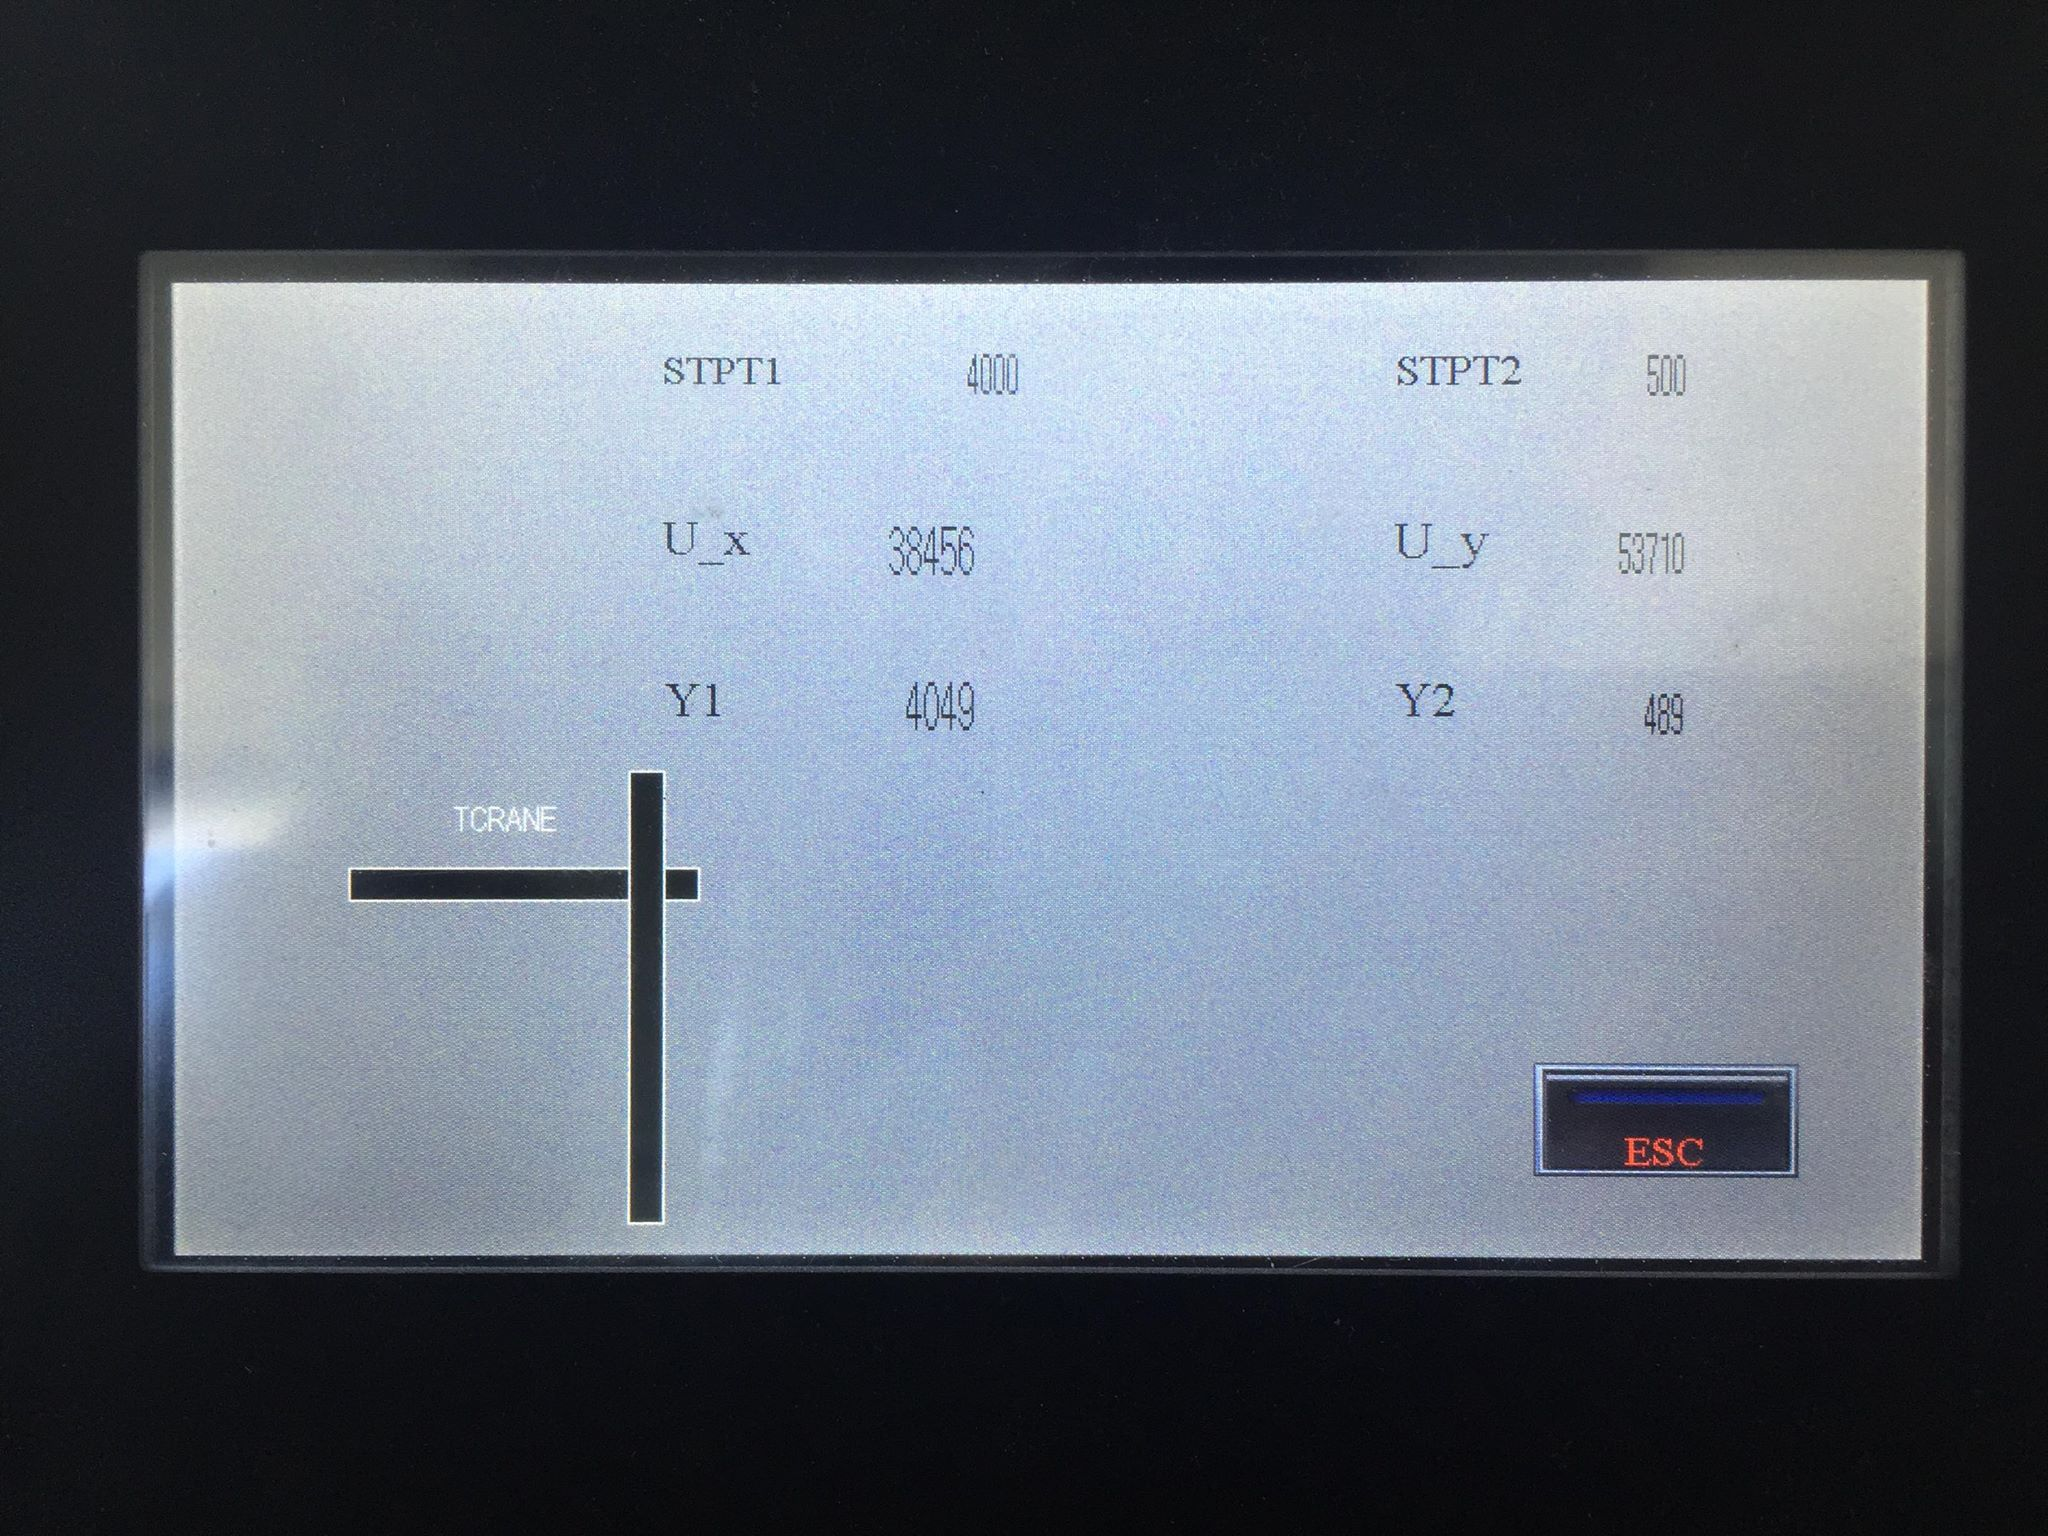
\includegraphics[scale=0.15]{./sections/inteco/images/reprezentacja_obiektu.jpg}
    \caption{Wizualizacja procesu}
\end{figure}

\section{Prezentacja sygnałów regulacji}
\label{inteco_wizualizacja_wykresy}
W procesie tworzenia panelu operatorskiego zawierało się również utworzenie ekranów zawierających przebiegi sygnałów procesowych. W celu umożliwienia wygodnej obserwacji sygnałów utworzone zostały cztery osobne ekrany zawierające wykresy sygnałów wyjść obiektu w osiach X oraz Y, a także wykresy sterowań dla każdego wyjścia.

\begin{figure}[H]
    \label{Wykresy::output_x}
    \centering
    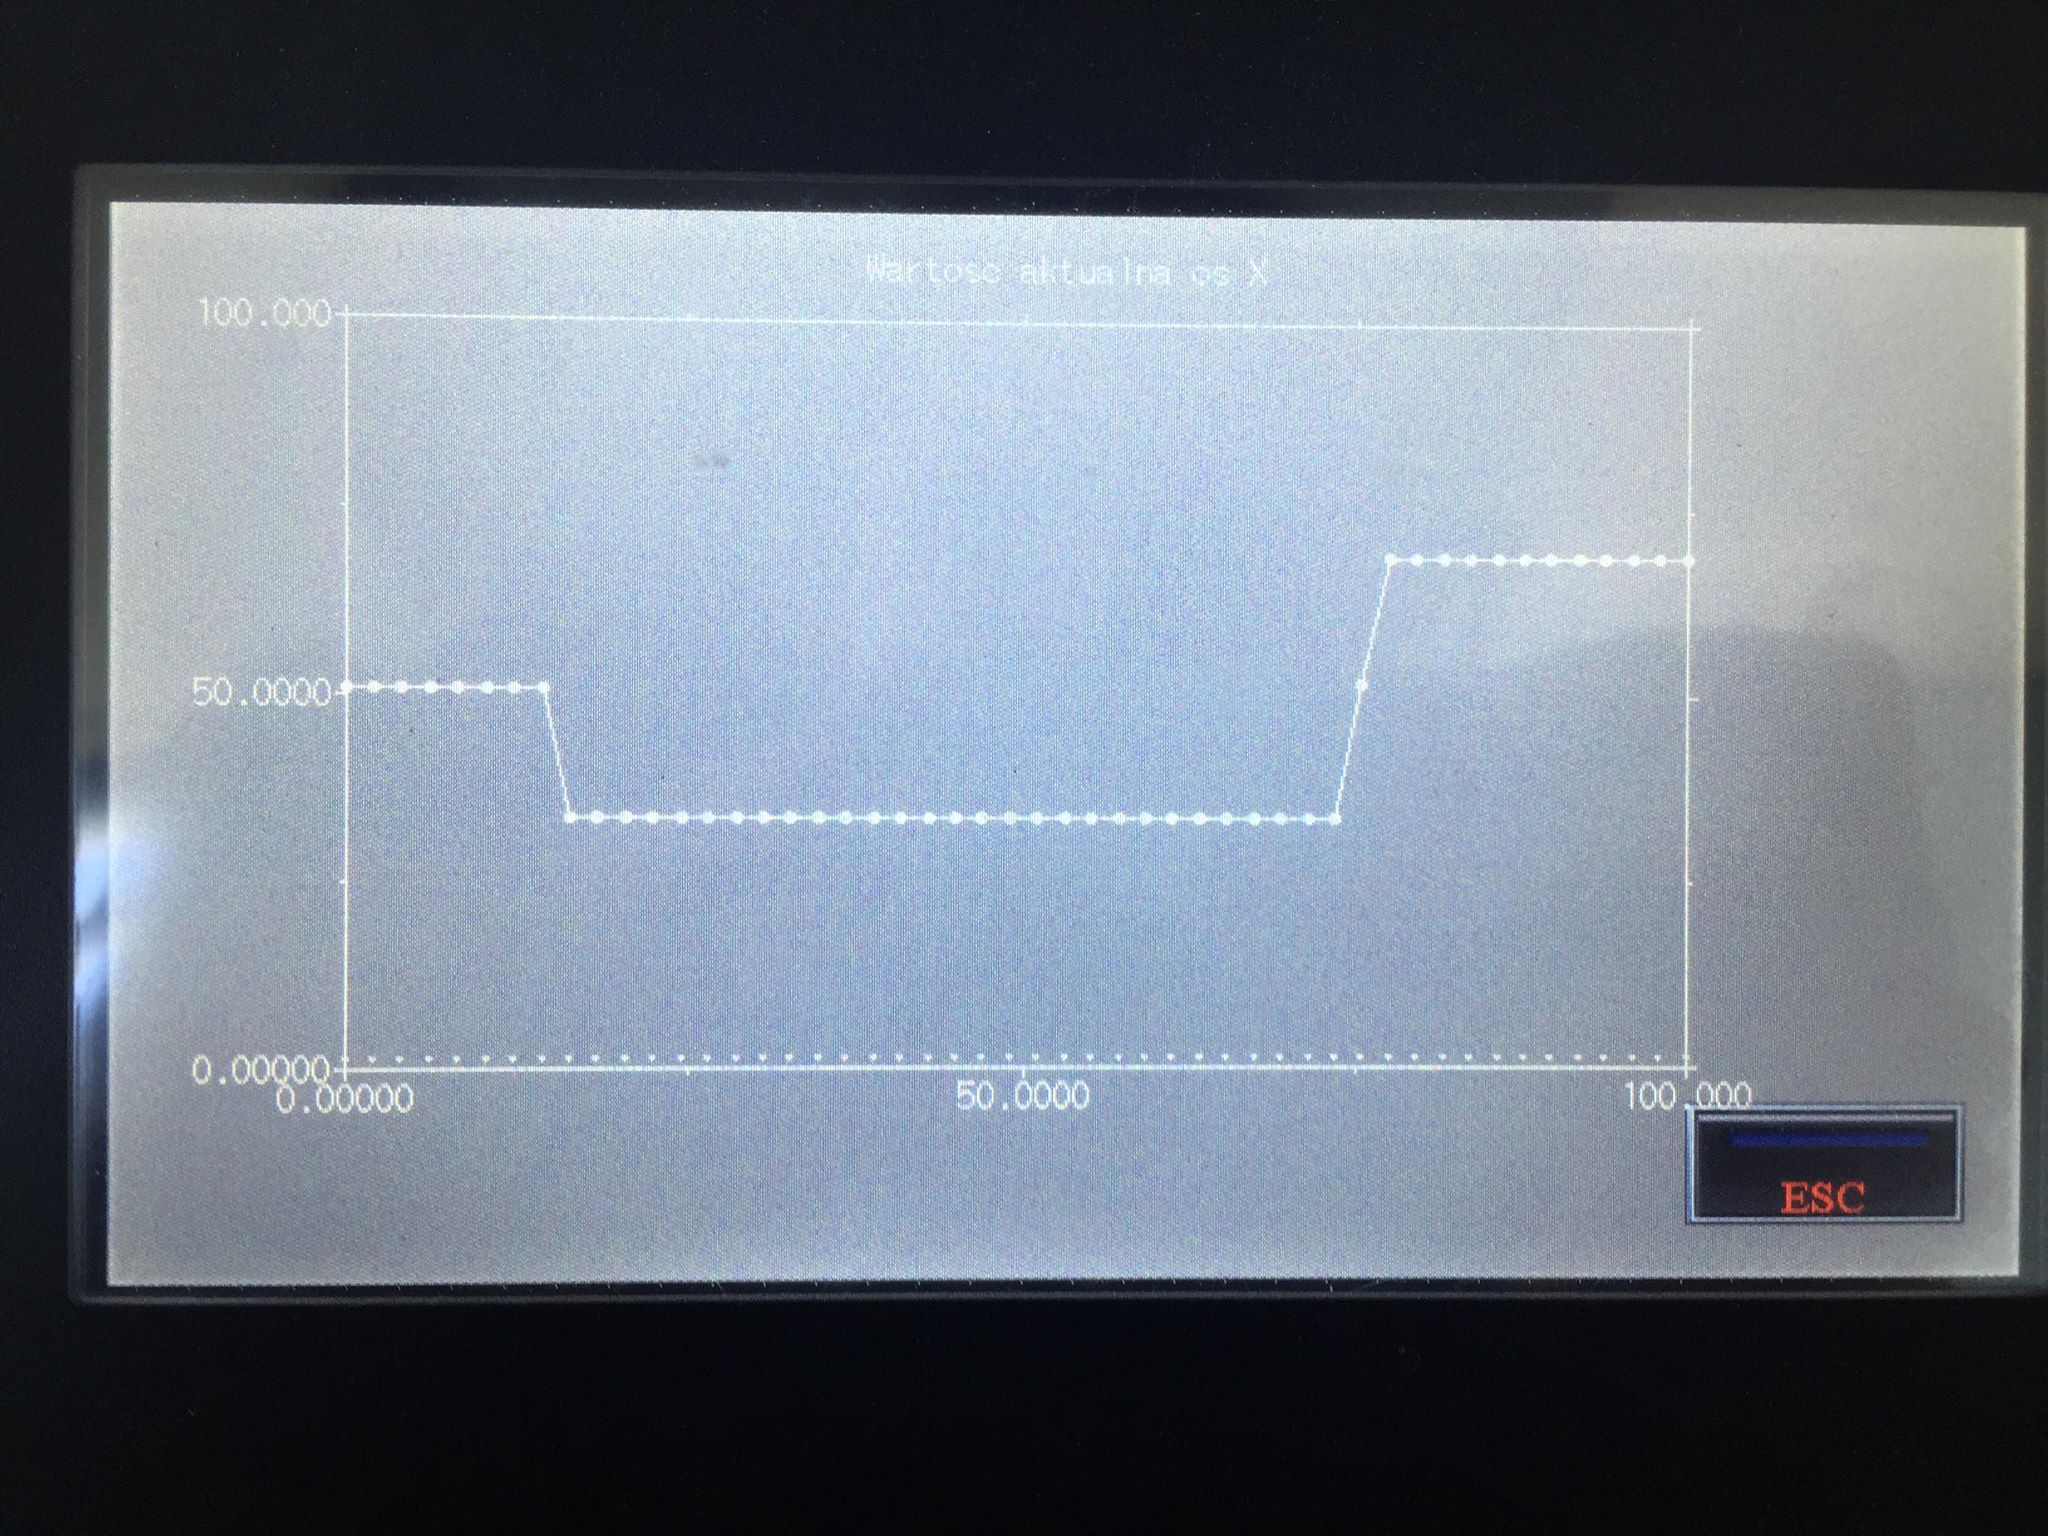
\includegraphics[scale=0.15]{./sections/inteco/images/output_x.jpg}
    \caption{Przebieg wyjścia dla osi X}
\end{figure}

\begin{figure}[H]
    \label{Wykres::input_x}
    \centering
    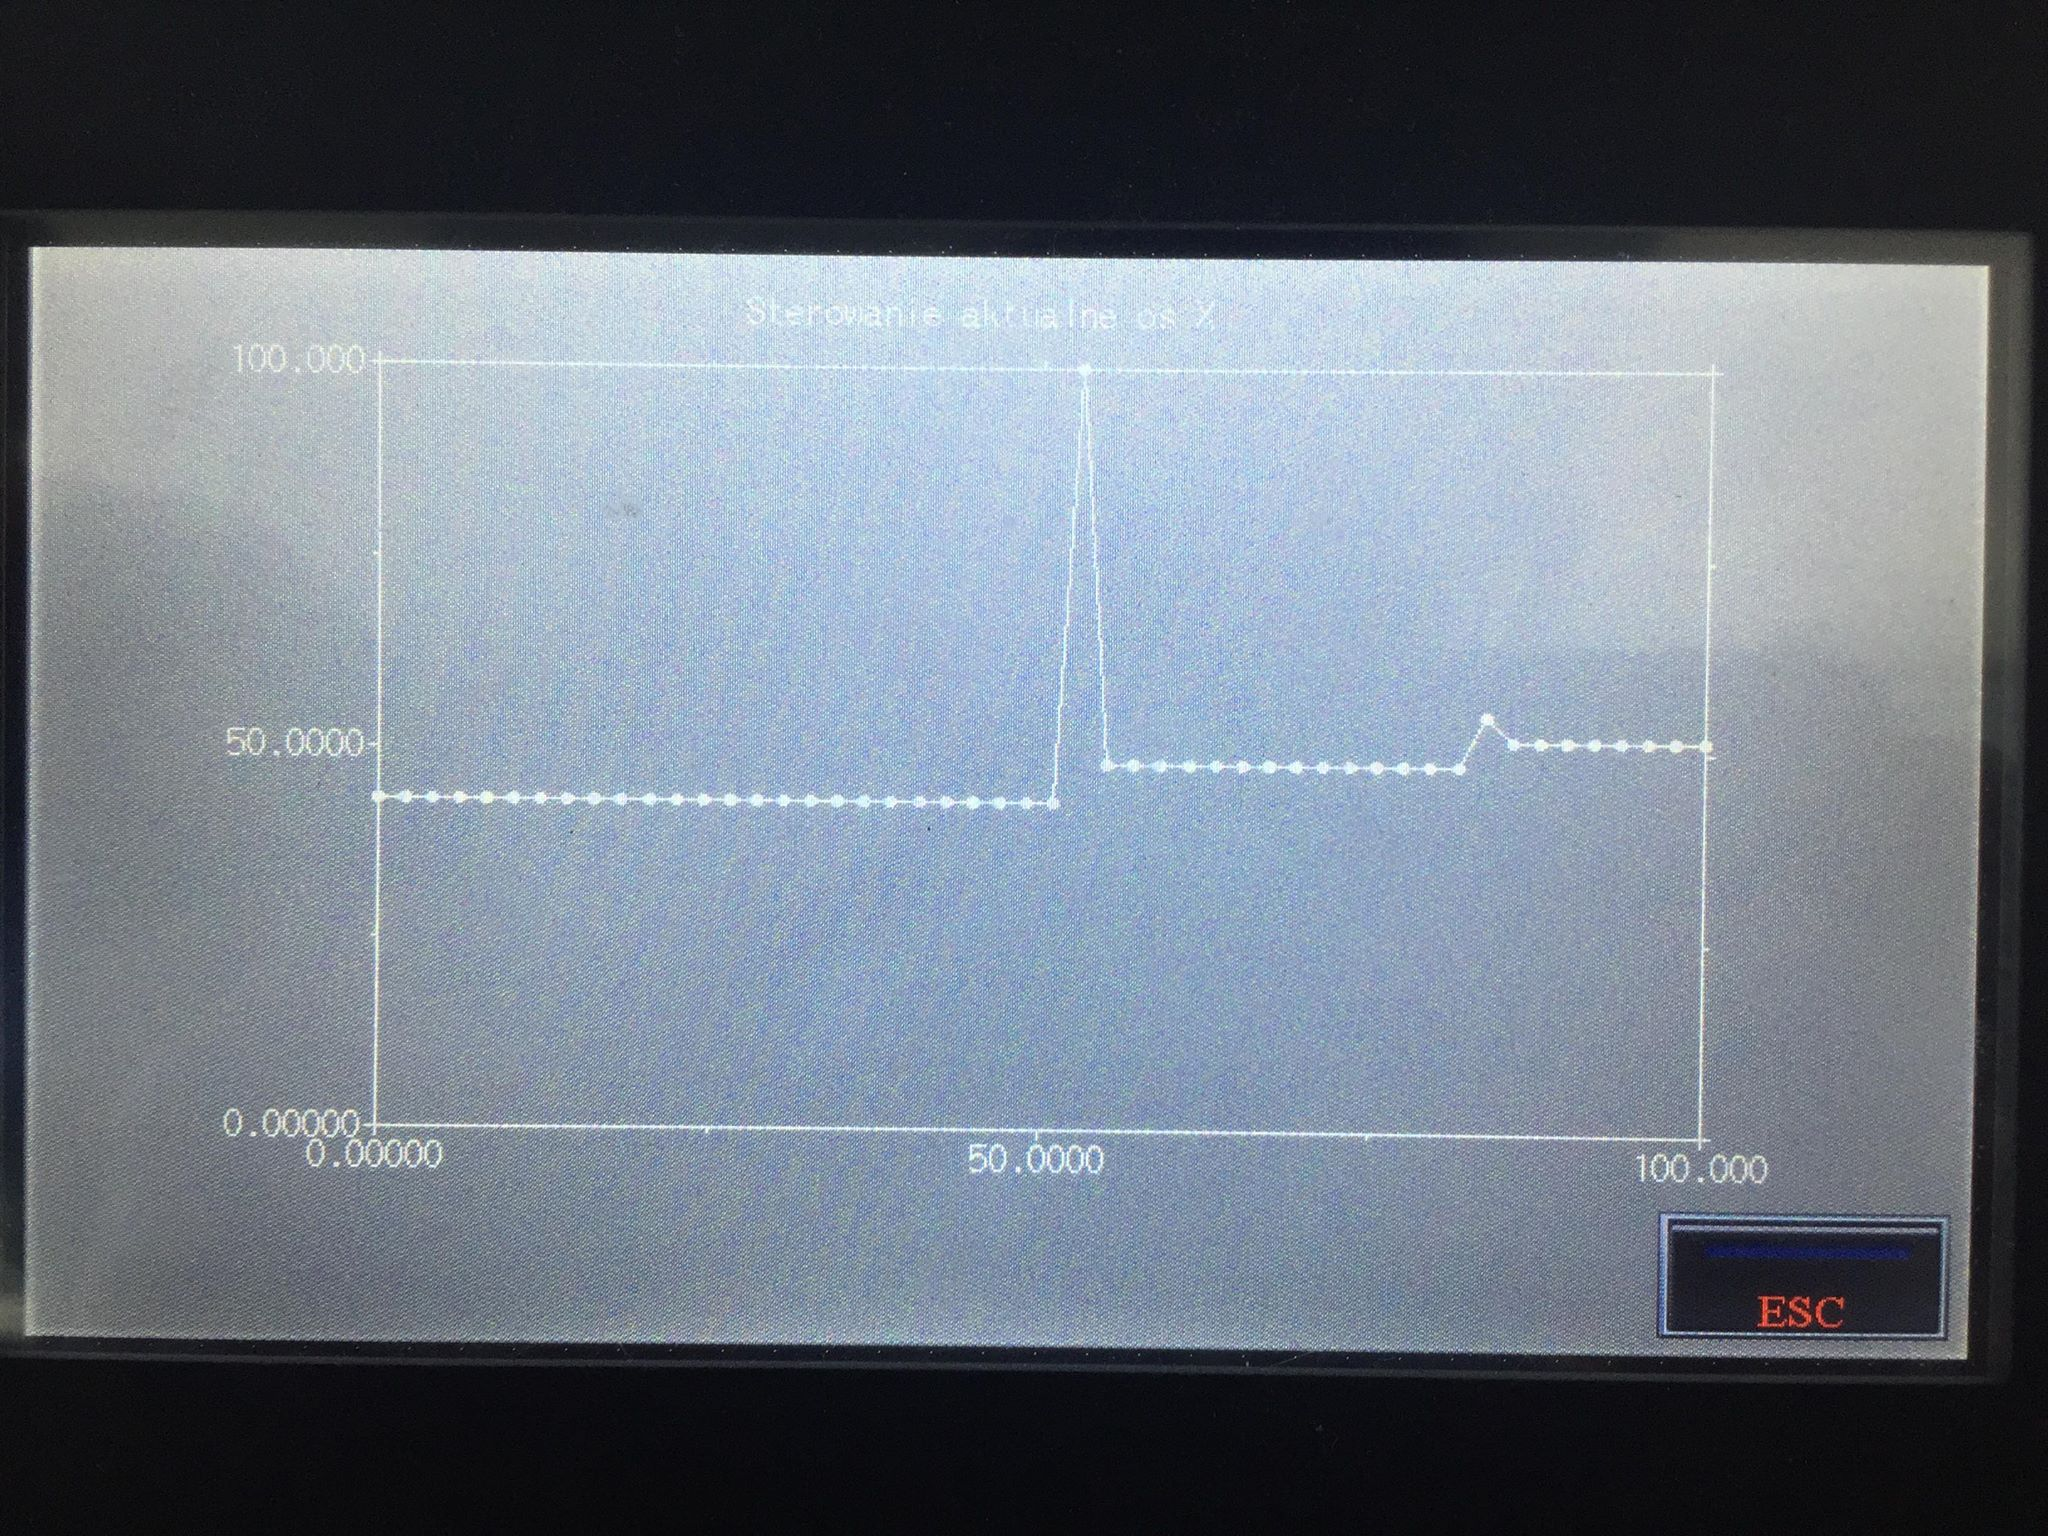
\includegraphics[scale=0.15]{./sections/inteco/images/input_x.jpg}
    \caption{Sterowanie dla osi X}
\end{figure}

\begin{figure}[H]
    \label{Wykres::output_y}
    \centering
    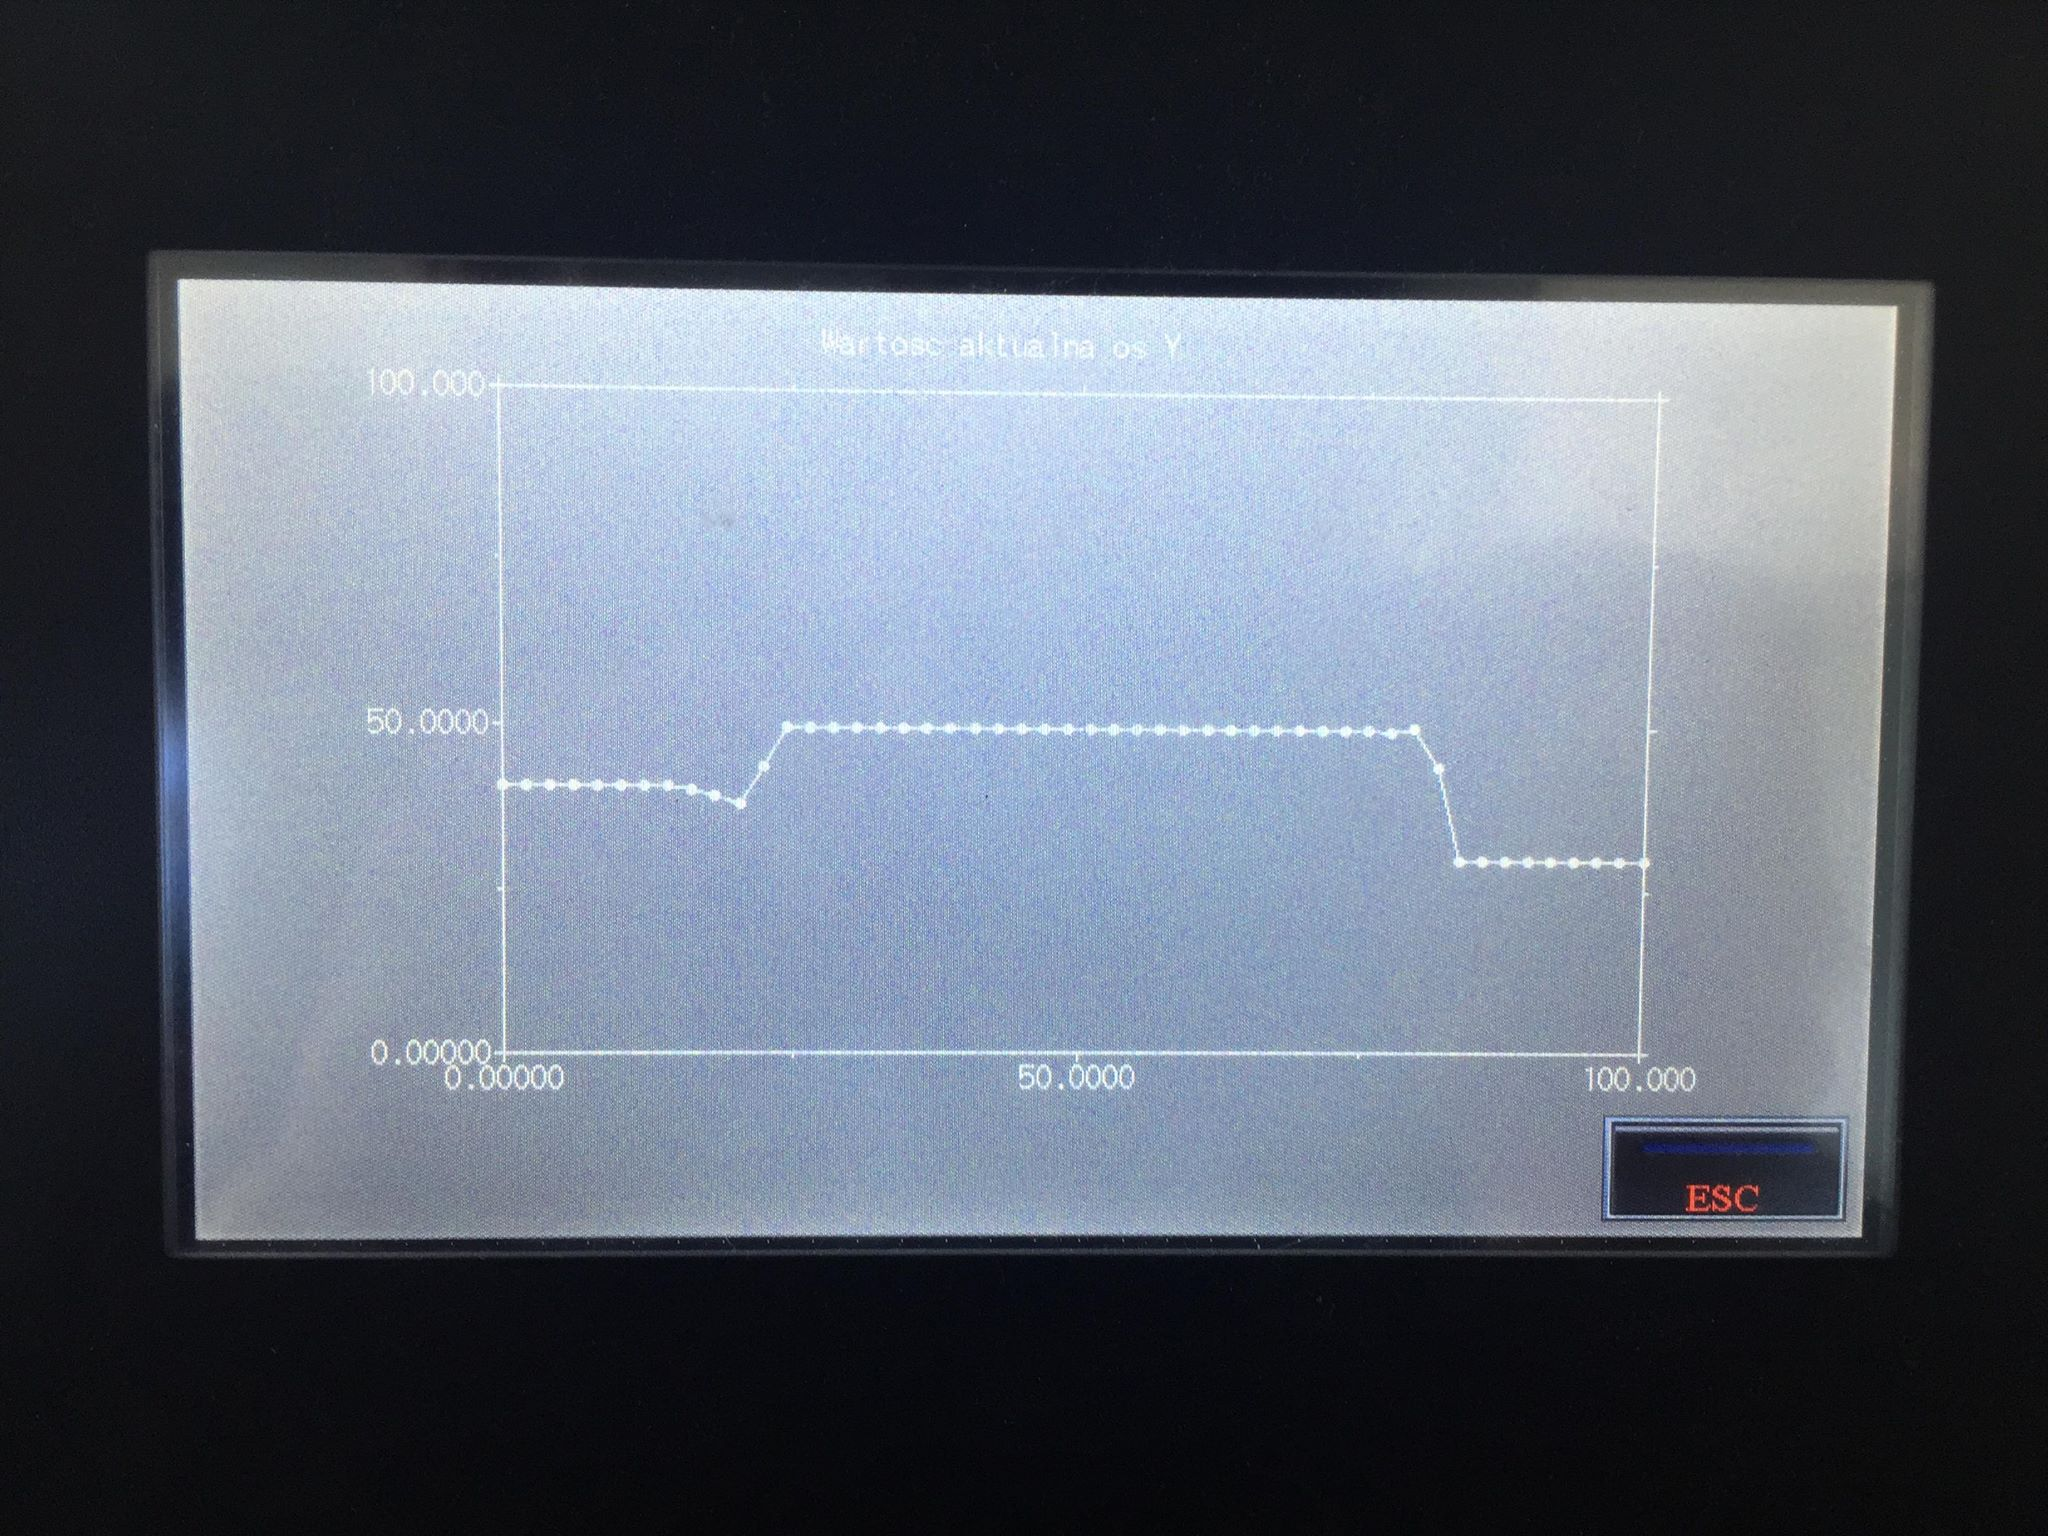
\includegraphics[scale=0.15]{./sections/inteco/images/output_y.jpg}
    \caption{Przebieg wyjścia dla osi Y}
\end{figure}

\begin{figure}[H]
    \label{Wykresy::input_y}
    \centering
    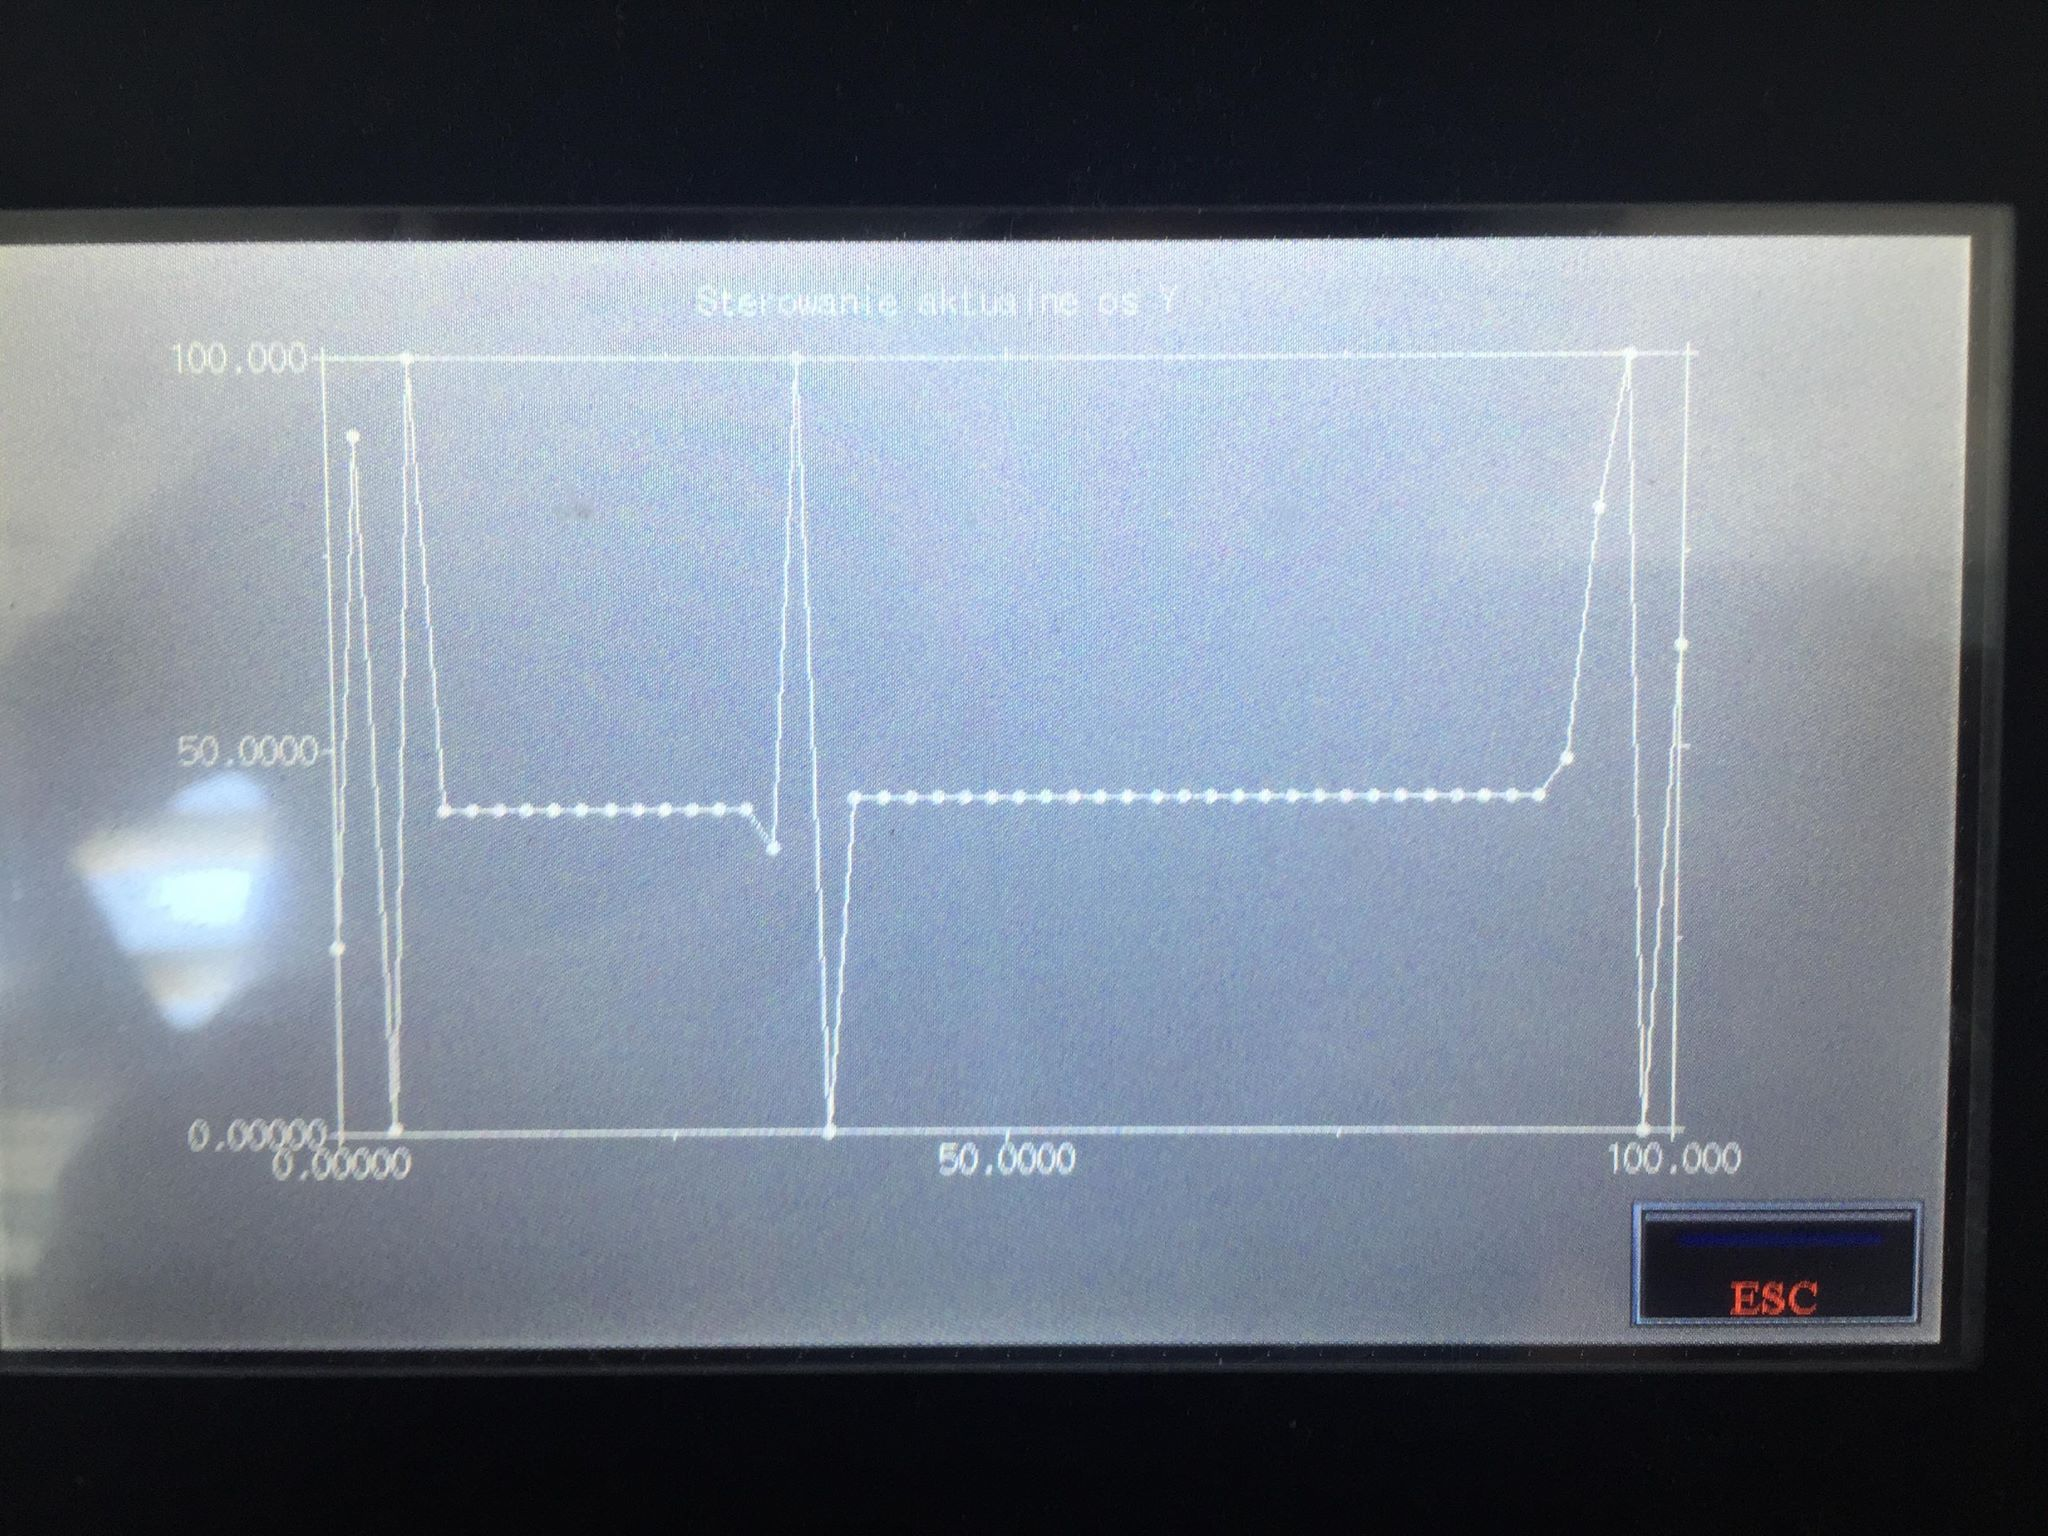
\includegraphics[scale=0.15]{./sections/inteco/images/input_y.jpg}
    \caption{Sterowanie dla osi Y}
\end{figure}

\section{Graf przejść automatu stanów}
\label{inteco_wizualizacja_automat}
W projekcie został również utworzony automat stanów procesu. Zmiany stanów następowały cyklicznie po upływie około 15 sekund. Ekran z automatem był zarówno ekranem początkowym, z którego można było przejść do każdego innego ekranu za pomocą przycisków znajdujących się po prawej stronie. Graf automatu znajduje się w centralnej części ekranu. Automat zawiera cztery stany. Dla stanu, w którym aktualnie znajduje się proces wyświetlany jest jego węzeł na grafie. Przykładowa prezentacja stanu procesu została przedstawiona na zdjęciach poniżej.

\begin{figure}[H]
    \label{automat_1}
    \centering
    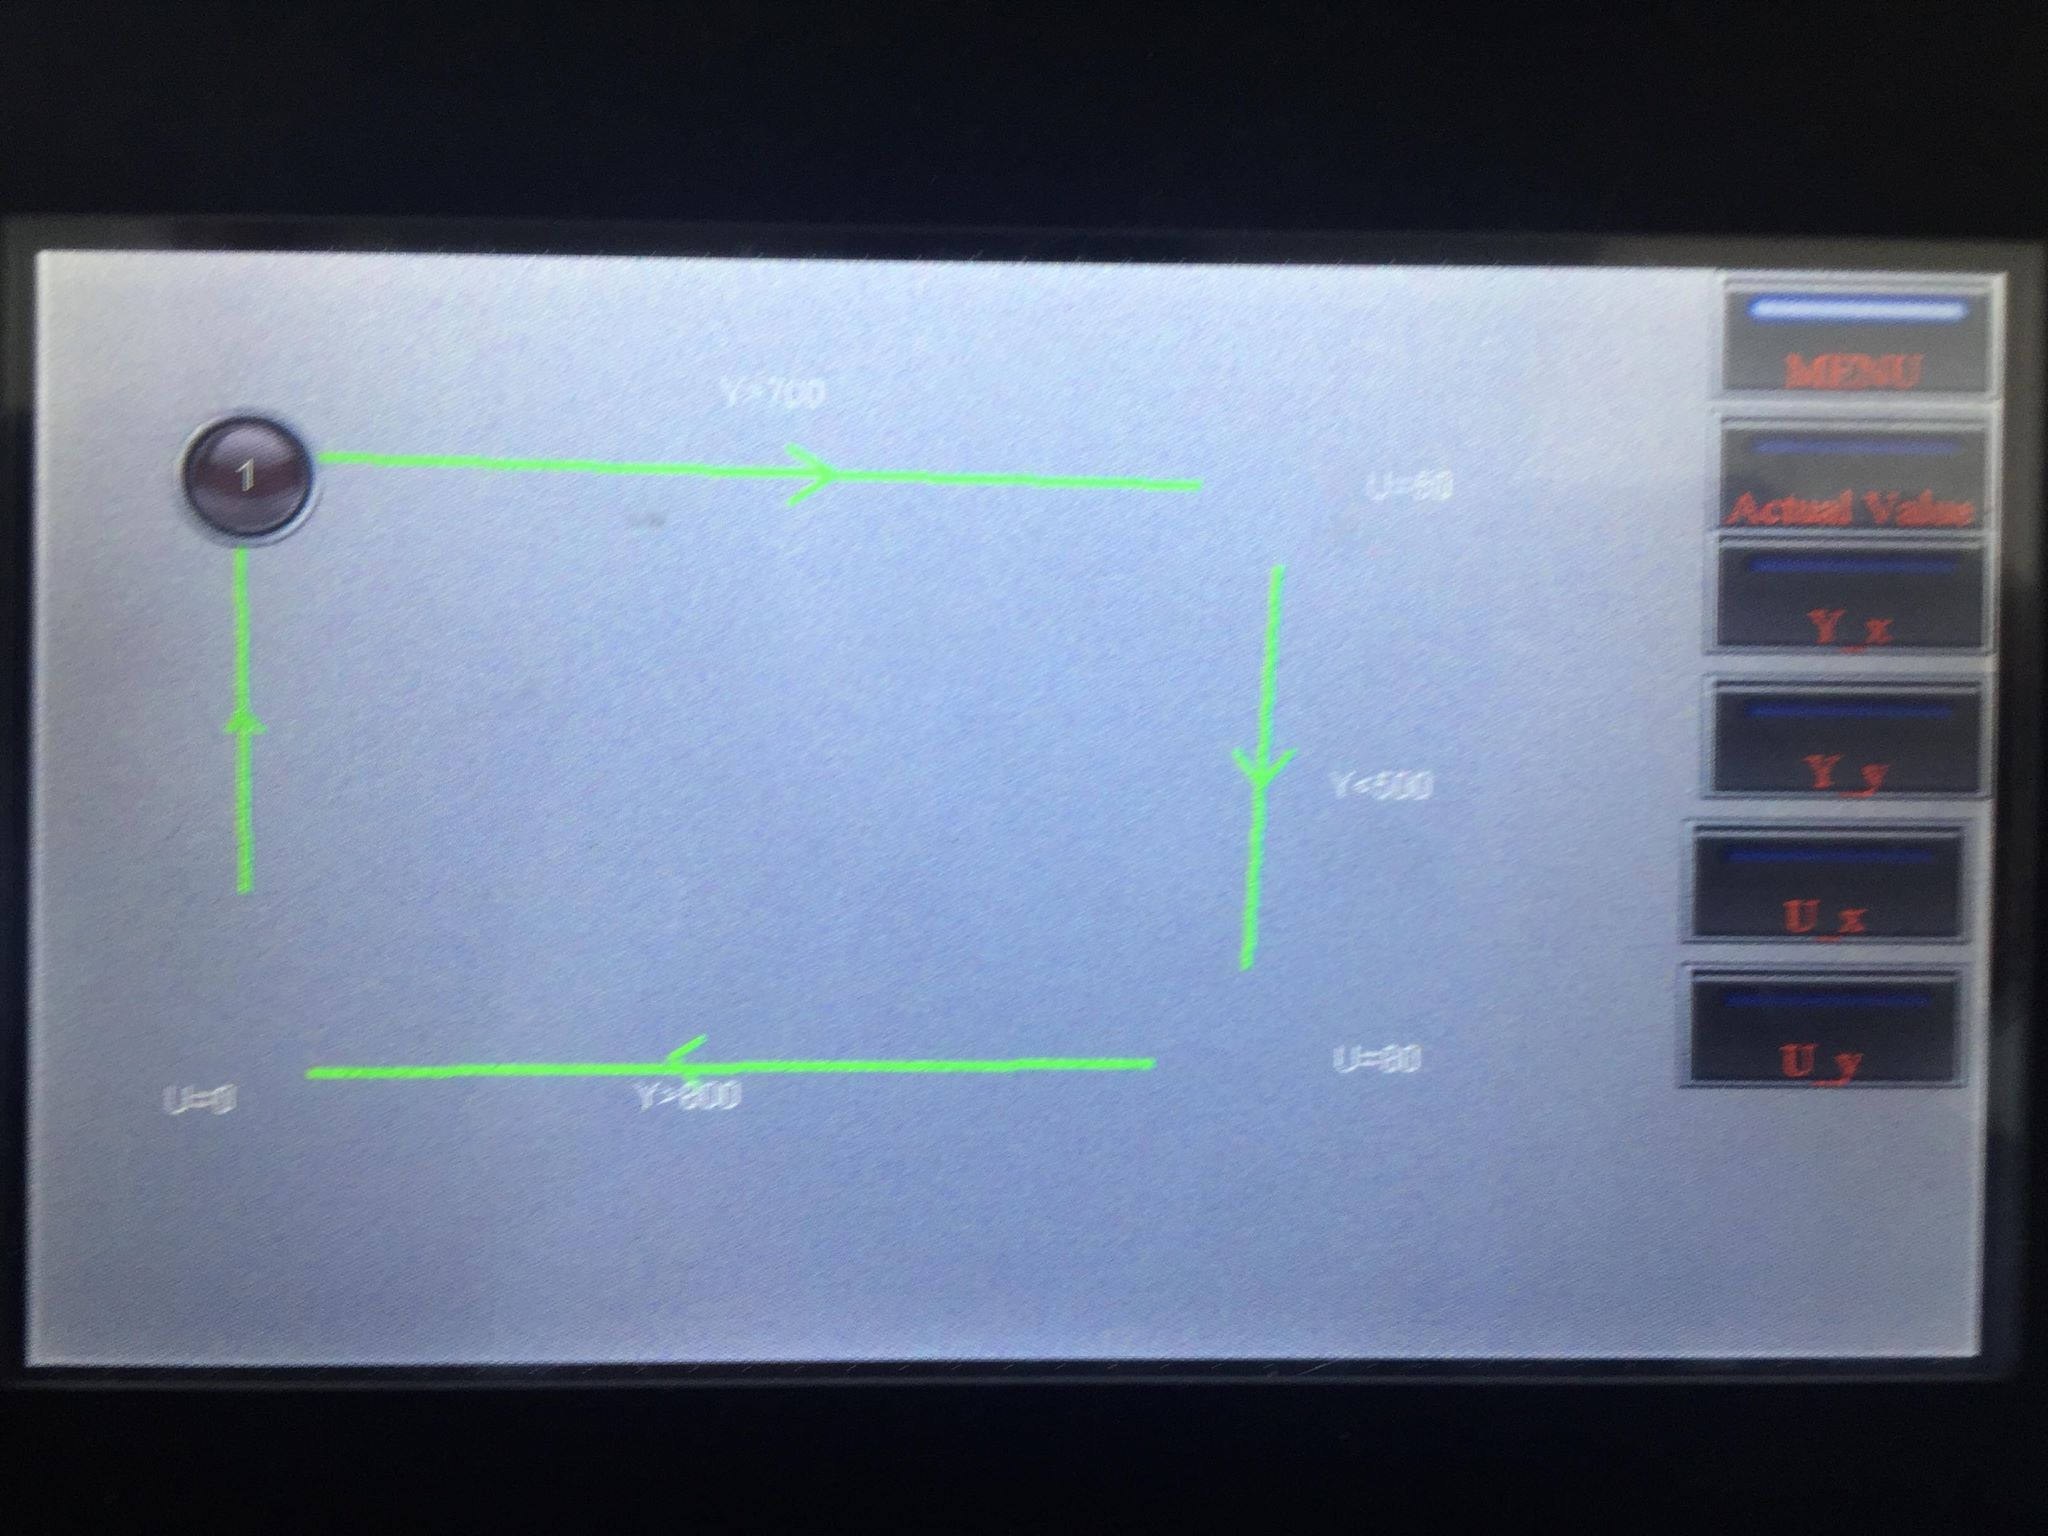
\includegraphics[scale=0.15]{./sections/inteco/images/automat1.jpg}
    \caption{Stan 1. procesu}
\end{figure}

\begin{figure}[H]
    \label{automat_3}
    \centering
    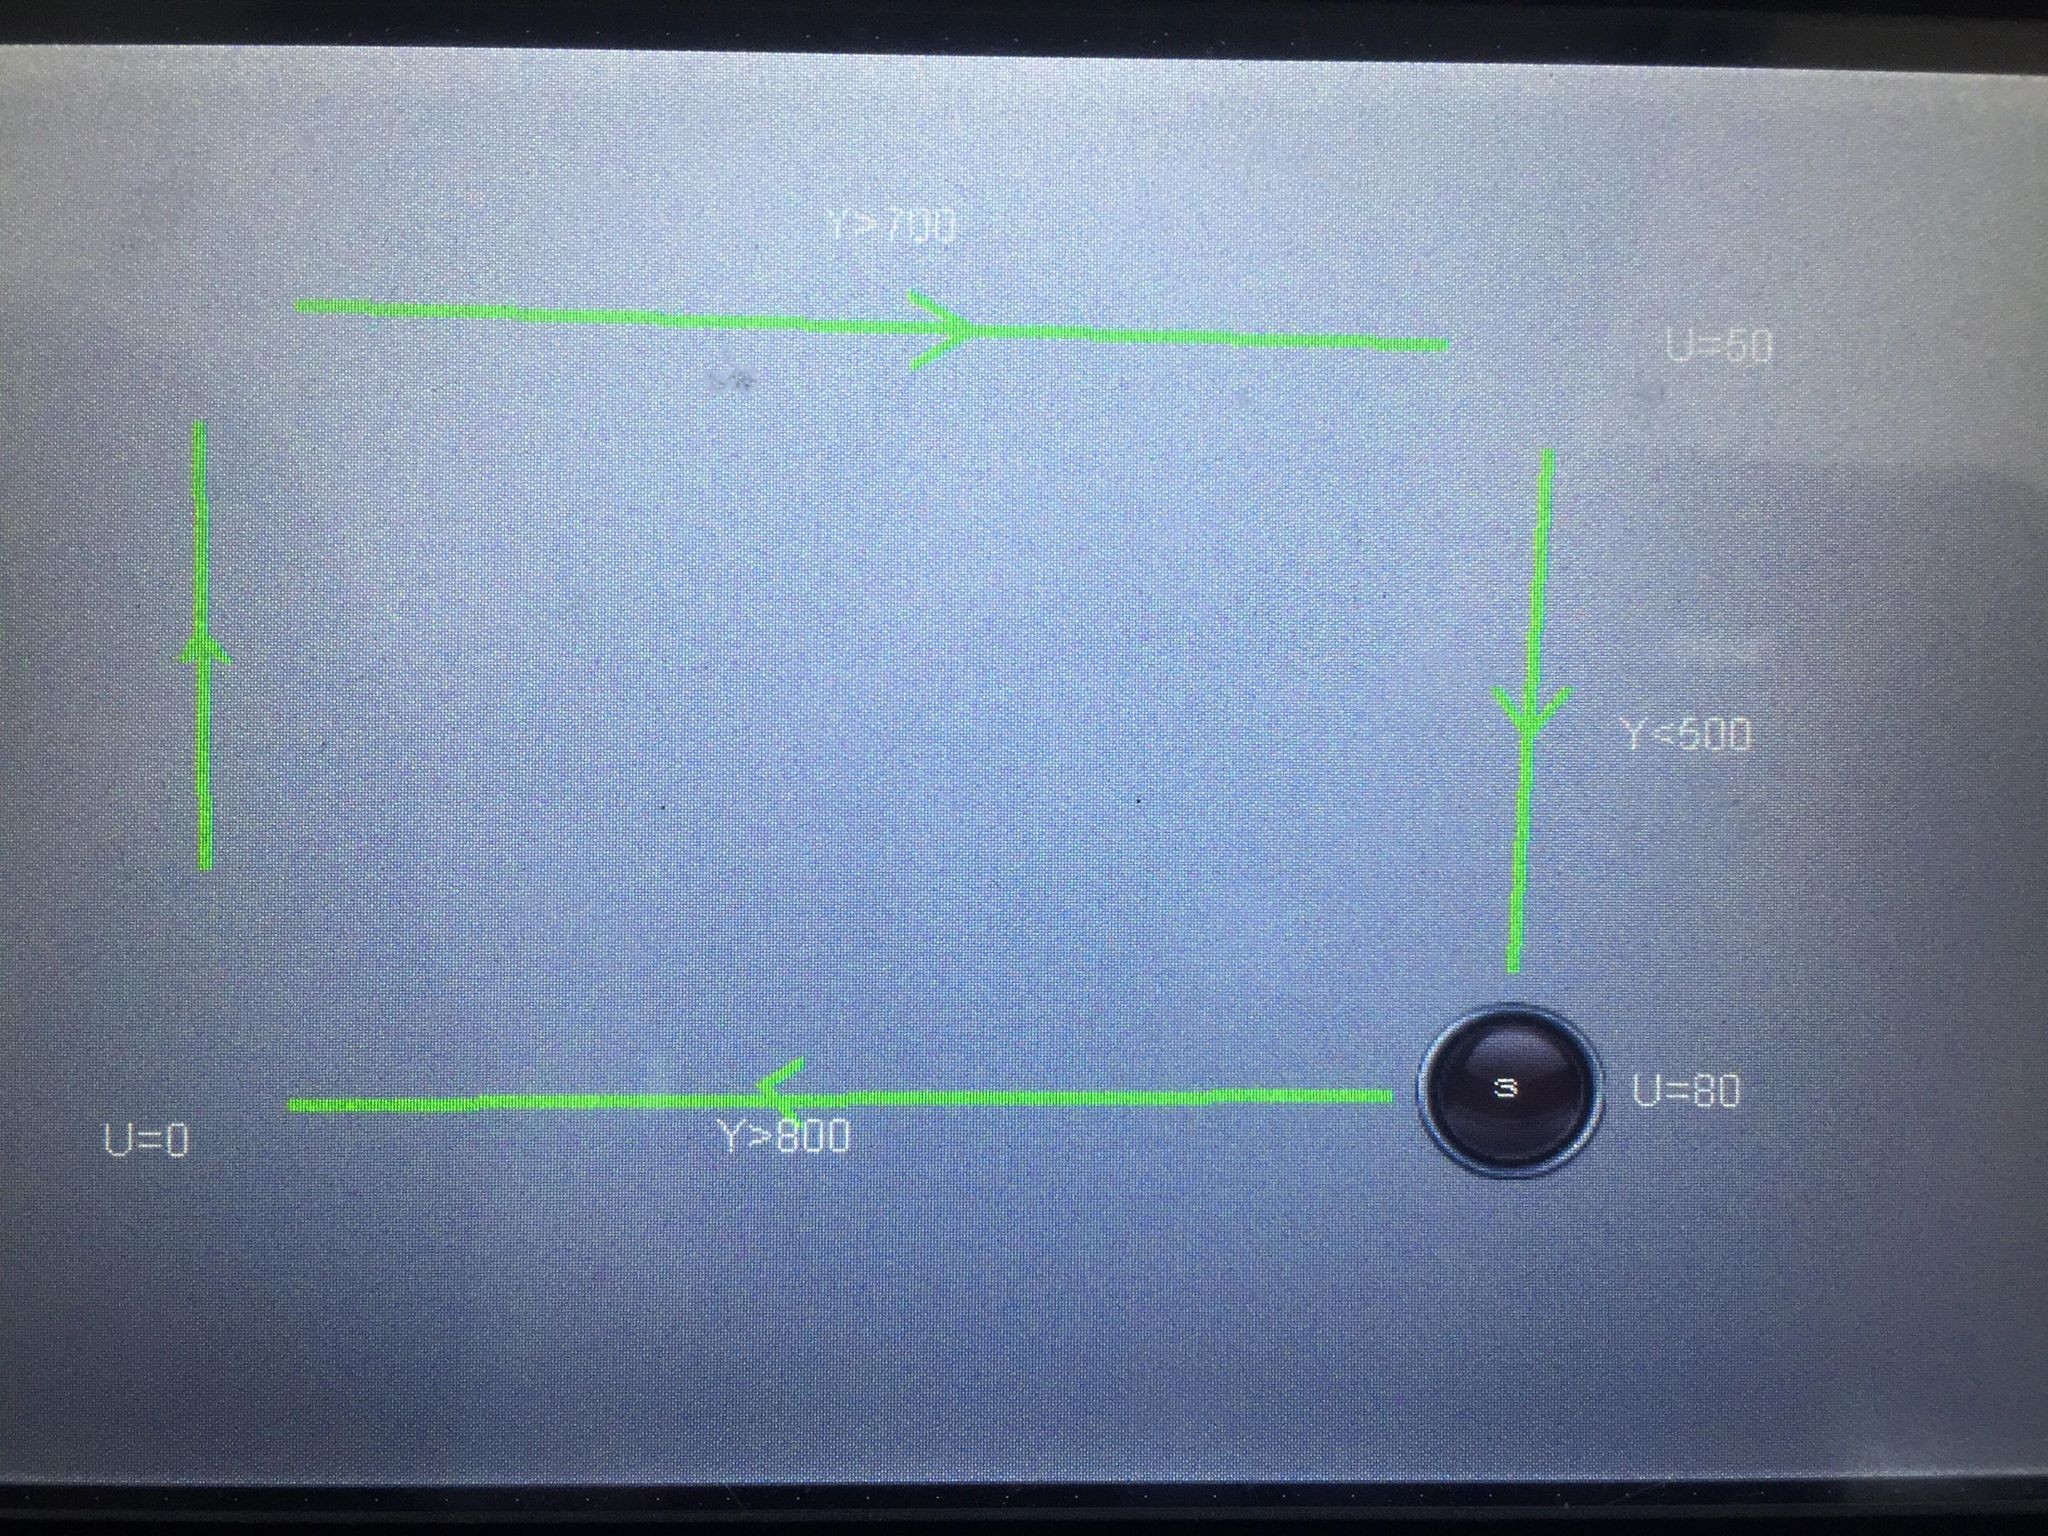
\includegraphics[scale=0.15]{./sections/inteco/images/automat3.jpg}
    \caption{Stan 3. procesu}
\end{figure}

\begin{figure}[H]
    \label{automat_4}
    \centering
    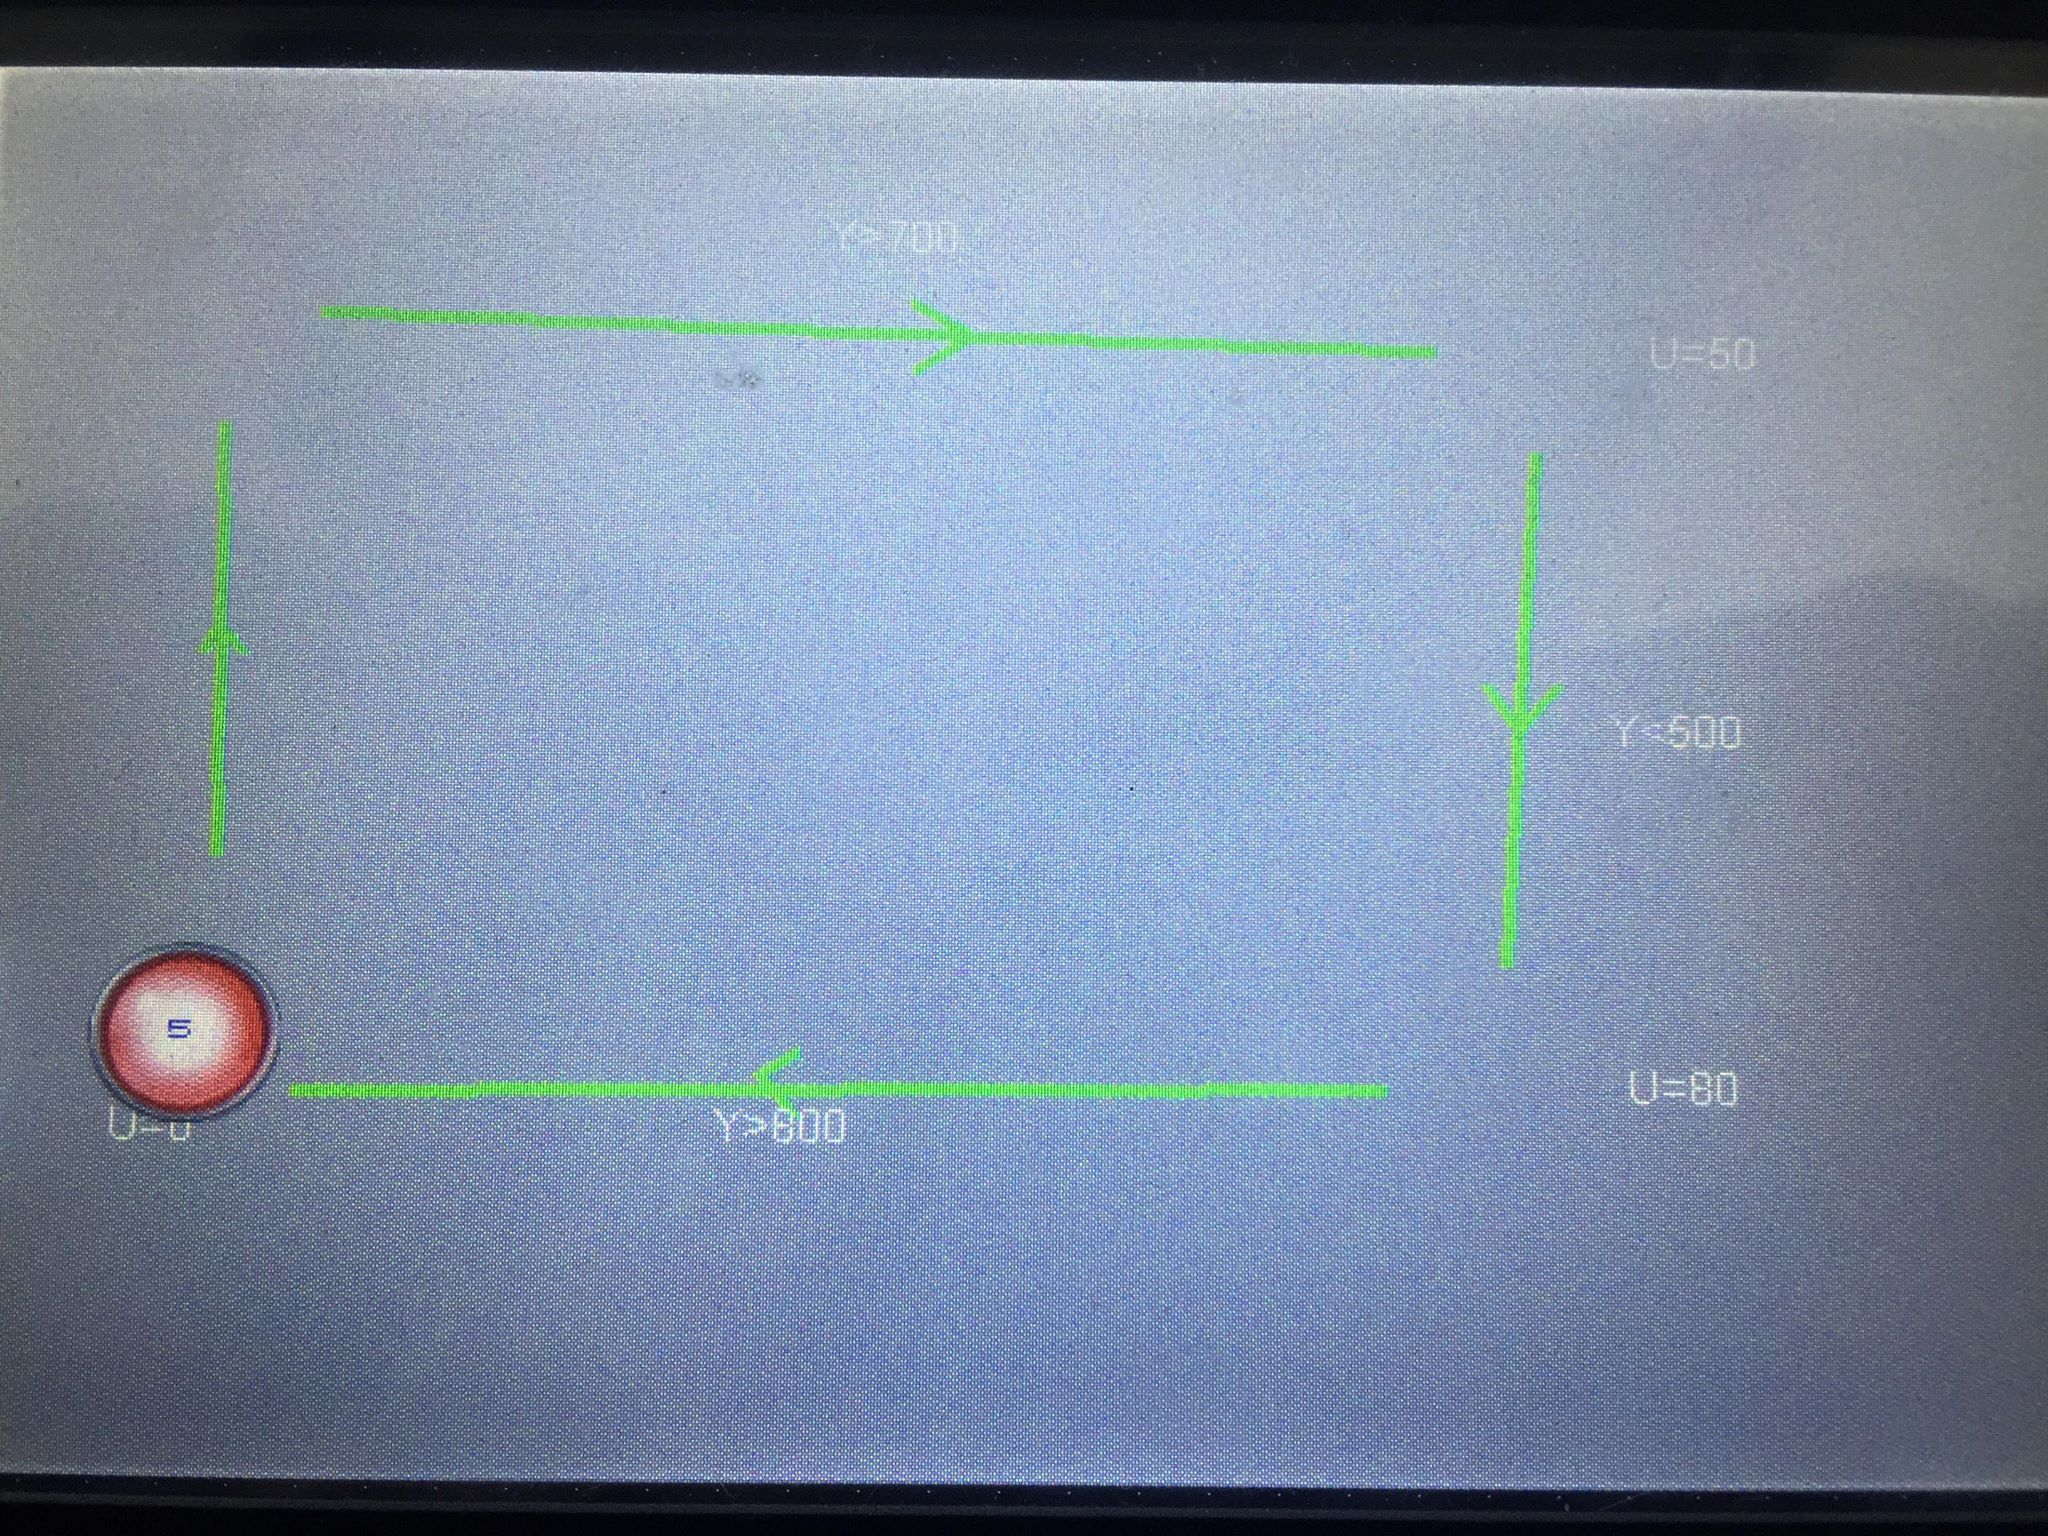
\includegraphics[scale=0.15]{./sections/inteco/images/automat5.jpg}
    \caption{Stan 4. procesu}
\end{figure}



%\chapter{Porównanie implementacji regulatora PID}
\label{inteco_porownanie}

\section{Implementacja regulatora PID przy pomocy wbudowanej w sterownik funkcji PID}
\label{inteco_pid_plc}

\section{Porównanie działania dwóch implementacji algorytmu}
\label{inteco_pid_porownanie}

\section{Wpływ ograniczeń na poszczególne implementacje regulatorów PID}
\label{inteco_pid_ograniczenia}


\end{document}